% Lines starting with a percent sign (%) are comments. LaTeX will 
% not process those lines. Similarly, everything after a percent 
% sign in a line is considered a comment. To produce a percent sign
% in the output, write \% (backslash followed by the percent sign). 
% ==================================================================
% Usage instructions:
% ------------------------------------------------------------------
% The file is heavily commented so that you know what the various
% commands do. Feel free to remove any comments you don't need from
% your own copy. When redistributing the example thesis file, please
% retain all the comments for the benefit of other thesis writers! 
% ==================================================================
% Compilation instructions: 
% ------------------------------------------------------------------
% Use pdflatex to compile! Input images are expected as PDF files.
% Example compilation:
% ------------------------------------------------------------------
% > pdflatex thesis-example.tex
% > bibtex thesis-example
% > pdflatex thesis-example.tex
% > pdflatex thesis-example.tex
% ------------------------------------------------------------------
% You need to run pdflatex multiple times so that all the cross-references
% are fixed. pdflatex will tell you if you need to re-run it (a warning
% will be issued)  
% ------------------------------------------------------------------
% Compilation has been tested to work in ukk.cs.hut.fi and kosh.hut.fi
% - if you have problems of missing .sty -files, then the local LaTeX
% environment does not have all the required packages installed.
% For example, when compiling in vipunen.hut.fi, you get an error that
% tikz.sty is missing - in this case you must either compile somewhere
% else, or you cannot use TikZ graphics in your thesis and must therefore
% remove or comment out the tikz package and all the tikz definitions. 
% ------------------------------------------------------------------

% General information
% ==================================================================
% Package documentation:
% 
% The comments often refer to package documentation. (Almost) all LaTeX
% packages have documentation accompanying them, so you can read the
% package documentation for further information. When a package 'xxx' is
% installed to your local LaTeX environment (the document compiles
% when you have \usepackage{xxx} and LaTeX does not complain), you can 
% find the documentation somewhere in the local LaTeX texmf directory
% hierarchy. In ukk.cs.hut.fi, this is /usr/texlive/2008/texmf-dist,
% and the documentation for the titlesec package (for example) can be 
% found at /usr/texlive/2008/texmf-dist/doc/latex/titlesec/titlesec.pdf.
% Most often the documentation is located as a PDF file in 
% /usr/texlive/2008/texmf-dist/doc/latex/xxx, where xxx is the package name; 
% however, documentation for TikZ is in
% /usr/texlive/2008/texmf-dist/doc/latex/generic/pgf/pgfmanual.pdf
% (this is because TikZ is a front-end for PGF, which is meant to be a 
% generic portable graphics format for LaTeX).
% You can try to look for the package manual using the ``find'' shell
% command in Linux machines; the find databases are up-to-date at least
% in ukk.cs.hut.fi. Just type ``find xxx'', where xxx is the package
% name, and you should find a documentation file.
% Note that in some packages, the documentation is in the DVI file
% format. In this case, you can copy the DVI file to your home directory,
% and convert it to PDF with the dvipdfm command (or you can read the
% DVI file directly with a DVI viewer).
% 
% If you can't find the documentation for a package, just try Googling
% for ``latex packagename''; most often you can get a direct link to the
% package manual in PDF format.
% ------------------------------------------------------------------


% Document class for the thesis is report
% ------------------------------------------------------------------
% You can change this but do so at your own risk - it may break other things.
% Note that the option pdftext is used for pdflatex; there is no
% pdflatex option. 
% ------------------------------------------------------------------
\documentclass[12pt,a4paper,oneside,pdftex]{report}

% The input files (tex files) are encoded with the latin-1 encoding 
% (ISO-8859-1 works). Change the latin1-option if you use UTF8 
% (at some point LaTeX did not work with UTF8, but I'm not sure
% what the current situation is) 
\usepackage[utf8]{inputenc}
% OT1 font encoding seems to work better than T1. Check the rendered
% PDF file to see if the fonts are encoded properly as vectors (instead
% of rendered bitmaps). You can do this by zooming very close to any letter 
% - if the letter is shown pixelated, you should change this setting 
% (try commenting out the entire line, for example).  
%\usepackage[OT1]{fontenc}
% The babel package provides hyphenating instructions for LaTeX. Give
% the languages you wish to use in your thesis as options to the babel
% package (as shown below). You can remove any language you are not
% going to use.
% Examples of valid language codes: english (or USenglish), british, 
% finnish, swedish; and so on.
\usepackage[finnish,swedish,english]{babel}


% Font selection
% ------------------------------------------------------------------
% The default LaTeX font is a very good font for rendering your 
% thesis. It is a very professional font, which will always be 
% accepted. 
% If you, however, wish to spicen up your thesis, you can try out
% these font variants by uncommenting one of the following lines
% (or by finding another font package). The fonts shown here are 
% all fonts that you could use in your thesis (not too silly). 
% Changing the font causes the layouts to shift a bit; you many
% need to manually adjust some layouts. Check the warning messages
% LaTeX gives you.
% ------------------------------------------------------------------
% To find another font, check out the font catalogue from
% http://www.tug.dk/FontCatalogue/mathfonts.html
% This link points to the list of fonts that support maths, but
% that's a fairly important point for master's theses.
% ------------------------------------------------------------------
% <rant>
% Remember, there is no excuse to use Comic Sans, ever, in any
% situation! (Well, maybe in speech bubbles in comics, but there 
% are better options for those too)
% </rant>

% \usepackage{palatino}
% \usepackage{tgpagella}



% Optional packages
% ------------------------------------------------------------------
% Select those packages that you need for your thesis. You may delete
% or comment the rest.

% Natbib allows you to select the format of the bibliography references.
% The first example uses numbered citations: 
\usepackage[square,sort&compress,numbers]{natbib}
% The second example uses author-year citations.
% If you use author-year citations, change the bibliography style (below); 
% acm style does not work with author-year citations.
% Also, you should use \citet (cite in text) when you wish to refer
% to the author directly (\citet{blaablaa} said blaa blaa), and 
% \citep when you wish to refer similarly than with numbered citations
% (It has been said that blaa blaa~\citep{blaablaa}).
% \usepackage[square]{natbib}

% The alltt package provides an all-teletype environment that acts
% like verbatim but you can use LaTeX commands in it. Uncomment if 
% you want to use this environment. 
% \usepackage{alltt}

% The eurosym package provides a euro symbol. Use with \euro{}
\usepackage{eurosym} 

% Verbatim provides a standard teletype environment that renderes
% the text exactly as written in the tex file. Useful for code
% snippets (although you can also use the listings package to get
% automatic code formatting). 
\usepackage{verbatim}

% The listing package provides automatic code formatting utilities
% so that you can copy-paste code examples and have them rendered
% nicely. See the package documentation for details.
% \usepackage{listings}

% The fancuvrb package provides fancier verbatim environments 
% (you can, for example, put borders around the verbatim text area
% and so on). See package for details.
% \usepackage{fancyvrb}

% Supertabular provides a tabular environment that can span multiple 
% pages. 
%\usepackage{supertabular}
% Longtable provides a tabular environment that can span multiple 
% pages. This is used in the example acronyms file. 
\usepackage{longtable}

% The fancyhdr package allows you to set your the page headers 
% manually, and allows you to add separator lines and so on. 
% Check the package documentation. 
% \usepackage{fancyhdr}

% Subfigure package allows you to use subfigures (i.e., many subfigures
% within one figure environment). These can have different labels and
% they are numbered automatically. Check the package documentation. 
\usepackage{subfigure}

% The titlesec package can be used to alter the look of the titles 
% of sections, chapters, and so on. This example uses the ``medium'' 
% package option which sets the titles to a medium size, making them
% a bit smaller than what is the default. You can fine-tune the 
% title fonts and sizes by using the package options. See the package
% documentation.
\usepackage[medium]{titlesec}

% The TikZ package allows you to create professional technical figures.
% The learning curve is quite steep, but it is definitely worth it if 
% you wish to have really good-looking technical figures. 
\usepackage{tikz}
\usepackage[titletoc]{appendix}
\usepackage{color}
\definecolor{AliceBlue}{rgb}{0.94,0.97,1.00}
\definecolor{AntiqueWhite1}{rgb}{1.00,0.94,0.86}
\definecolor{AntiqueWhite2}{rgb}{0.93,0.87,0.80}
\definecolor{AntiqueWhite3}{rgb}{0.80,0.75,0.69}
\definecolor{AntiqueWhite4}{rgb}{0.55,0.51,0.47}
\definecolor{AntiqueWhite}{rgb}{0.98,0.92,0.84}
\definecolor{BlanchedAlmond}{rgb}{1.00,0.92,0.80}
\definecolor{BlueViolet}{rgb}{0.54,0.17,0.89}
\definecolor{CadetBlue1}{rgb}{0.60,0.96,1.00}
\definecolor{CadetBlue2}{rgb}{0.56,0.90,0.93}
\definecolor{CadetBlue3}{rgb}{0.48,0.77,0.80}
\definecolor{CadetBlue4}{rgb}{0.33,0.53,0.55}
\definecolor{CadetBlue}{rgb}{0.37,0.62,0.63}
\definecolor{CornflowerBlue}{rgb}{0.39,0.58,0.93}
\definecolor{DarkBlue}{rgb}{0.00,0.00,0.55}
\definecolor{DarkCyan}{rgb}{0.00,0.55,0.55}
\definecolor{DarkGoldenrod1}{rgb}{1.00,0.73,0.06}
\definecolor{DarkGoldenrod2}{rgb}{0.93,0.68,0.05}
\definecolor{DarkGoldenrod3}{rgb}{0.80,0.58,0.05}
\definecolor{DarkGoldenrod4}{rgb}{0.55,0.40,0.03}
\definecolor{DarkGoldenrod}{rgb}{0.72,0.53,0.04}
\definecolor{DarkGray}{rgb}{0.66,0.66,0.66}
\definecolor{DarkGreen}{rgb}{0.00,0.39,0.00}
\definecolor{DarkGrey}{rgb}{0.66,0.66,0.66}
\definecolor{DarkKhaki}{rgb}{0.74,0.72,0.42}
\definecolor{DarkMagenta}{rgb}{0.55,0.00,0.55}
\definecolor{DarkOliveGreen1}{rgb}{0.79,1.00,0.44}
\definecolor{DarkOliveGreen2}{rgb}{0.74,0.93,0.41}
\definecolor{DarkOliveGreen3}{rgb}{0.64,0.80,0.35}
\definecolor{DarkOliveGreen4}{rgb}{0.43,0.55,0.24}
\definecolor{DarkOliveGreen}{rgb}{0.33,0.42,0.18}
\definecolor{DarkOrange1}{rgb}{1.00,0.50,0.00}
\definecolor{DarkOrange2}{rgb}{0.93,0.46,0.00}
\definecolor{DarkOrange3}{rgb}{0.80,0.40,0.00}
\definecolor{DarkOrange4}{rgb}{0.55,0.27,0.00}
\definecolor{DarkOrange}{rgb}{1.00,0.55,0.00}
\definecolor{DarkOrchid1}{rgb}{0.75,0.24,1.00}
\definecolor{DarkOrchid2}{rgb}{0.70,0.23,0.93}
\definecolor{DarkOrchid3}{rgb}{0.60,0.20,0.80}
\definecolor{DarkOrchid4}{rgb}{0.41,0.13,0.55}
\definecolor{DarkOrchid}{rgb}{0.60,0.20,0.80}
\definecolor{DarkRed}{rgb}{0.55,0.00,0.00}
\definecolor{DarkSalmon}{rgb}{0.91,0.59,0.48}
\definecolor{DarkSeaGreen1}{rgb}{0.76,1.00,0.76}
\definecolor{DarkSeaGreen2}{rgb}{0.71,0.93,0.71}
\definecolor{DarkSeaGreen3}{rgb}{0.61,0.80,0.61}
\definecolor{DarkSeaGreen4}{rgb}{0.41,0.55,0.41}
\definecolor{DarkSeaGreen}{rgb}{0.56,0.74,0.56}
\definecolor{DarkSlateBlue}{rgb}{0.28,0.24,0.55}
\definecolor{DarkSlateGray1}{rgb}{0.59,1.00,1.00}
\definecolor{DarkSlateGray2}{rgb}{0.55,0.93,0.93}
\definecolor{DarkSlateGray3}{rgb}{0.47,0.80,0.80}
\definecolor{DarkSlateGray4}{rgb}{0.32,0.55,0.55}
\definecolor{DarkSlateGray}{rgb}{0.18,0.31,0.31}
\definecolor{DarkSlateGrey}{rgb}{0.18,0.31,0.31}
\definecolor{DarkTurquoise}{rgb}{0.00,0.81,0.82}
\definecolor{DarkViolet}{rgb}{0.58,0.00,0.83}
\definecolor{DeepPink1}{rgb}{1.00,0.08,0.58}
\definecolor{DeepPink2}{rgb}{0.93,0.07,0.54}
\definecolor{DeepPink3}{rgb}{0.80,0.06,0.46}
\definecolor{DeepPink4}{rgb}{0.55,0.04,0.31}
\definecolor{DeepPink}{rgb}{1.00,0.08,0.58}
\definecolor{DeepSkyBlue1}{rgb}{0.00,0.75,1.00}
\definecolor{DeepSkyBlue2}{rgb}{0.00,0.70,0.93}
\definecolor{DeepSkyBlue3}{rgb}{0.00,0.60,0.80}
\definecolor{DeepSkyBlue4}{rgb}{0.00,0.41,0.55}
\definecolor{DeepSkyBlue}{rgb}{0.00,0.75,1.00}
\definecolor{DimGray}{rgb}{0.41,0.41,0.41}
\definecolor{DimGrey}{rgb}{0.41,0.41,0.41}
\definecolor{DodgerBlue1}{rgb}{0.12,0.56,1.00}
\definecolor{DodgerBlue2}{rgb}{0.11,0.53,0.93}
\definecolor{DodgerBlue3}{rgb}{0.09,0.45,0.80}
\definecolor{DodgerBlue4}{rgb}{0.06,0.31,0.55}
\definecolor{DodgerBlue}{rgb}{0.12,0.56,1.00}
\definecolor{FloralWhite}{rgb}{1.00,0.98,0.94}
\definecolor{ForestGreen}{rgb}{0.13,0.55,0.13}
\definecolor{GhostWhite}{rgb}{0.97,0.97,1.00}
\definecolor{GreenYellow}{rgb}{0.68,1.00,0.18}
\definecolor{HotPink1}{rgb}{1.00,0.43,0.71}
\definecolor{HotPink2}{rgb}{0.93,0.42,0.65}
\definecolor{HotPink3}{rgb}{0.80,0.38,0.56}
\definecolor{HotPink4}{rgb}{0.55,0.23,0.38}
\definecolor{HotPink}{rgb}{1.00,0.41,0.71}
\definecolor{IndianRed1}{rgb}{1.00,0.42,0.42}
\definecolor{IndianRed2}{rgb}{0.93,0.39,0.39}
\definecolor{IndianRed3}{rgb}{0.80,0.33,0.33}
\definecolor{IndianRed4}{rgb}{0.55,0.23,0.23}
\definecolor{IndianRed}{rgb}{0.80,0.36,0.36}
\definecolor{LavenderBlush1}{rgb}{1.00,0.94,0.96}
\definecolor{LavenderBlush2}{rgb}{0.93,0.88,0.90}
\definecolor{LavenderBlush3}{rgb}{0.80,0.76,0.77}
\definecolor{LavenderBlush4}{rgb}{0.55,0.51,0.53}
\definecolor{LavenderBlush}{rgb}{1.00,0.94,0.96}
\definecolor{LawnGreen}{rgb}{0.49,0.99,0.00}
\definecolor{LemonChiffon1}{rgb}{1.00,0.98,0.80}
\definecolor{LemonChiffon2}{rgb}{0.93,0.91,0.75}
\definecolor{LemonChiffon3}{rgb}{0.80,0.79,0.65}
\definecolor{LemonChiffon4}{rgb}{0.55,0.54,0.44}
\definecolor{LemonChiffon}{rgb}{1.00,0.98,0.80}
\definecolor{LightBlue1}{rgb}{0.75,0.94,1.00}
\definecolor{LightBlue2}{rgb}{0.70,0.87,0.93}
\definecolor{LightBlue3}{rgb}{0.60,0.75,0.80}
\definecolor{LightBlue4}{rgb}{0.41,0.51,0.55}
\definecolor{LightBlue}{rgb}{0.68,0.85,0.90}
\definecolor{LightCoral}{rgb}{0.94,0.50,0.50}
\definecolor{LightCyan1}{rgb}{0.88,1.00,1.00}
\definecolor{LightCyan2}{rgb}{0.82,0.93,0.93}
\definecolor{LightCyan3}{rgb}{0.71,0.80,0.80}
\definecolor{LightCyan4}{rgb}{0.48,0.55,0.55}
\definecolor{LightCyan}{rgb}{0.88,1.00,1.00}
\definecolor{LightGoldenrod1}{rgb}{1.00,0.93,0.55}
\definecolor{LightGoldenrod2}{rgb}{0.93,0.86,0.51}
\definecolor{LightGoldenrod3}{rgb}{0.80,0.75,0.44}
\definecolor{LightGoldenrod4}{rgb}{0.55,0.51,0.30}
\definecolor{LightGoldenrodYellow}{rgb}{0.98,0.98,0.82}
\definecolor{LightGoldenrod}{rgb}{0.93,0.87,0.51}
\definecolor{LightGray}{rgb}{0.83,0.83,0.83}
\definecolor{LightGreen}{rgb}{0.56,0.93,0.56}
\definecolor{LightGrey}{rgb}{0.83,0.83,0.83}
\definecolor{LightPink1}{rgb}{1.00,0.68,0.73}
\definecolor{LightPink2}{rgb}{0.93,0.64,0.68}
\definecolor{LightPink3}{rgb}{0.80,0.55,0.58}
\definecolor{LightPink4}{rgb}{0.55,0.37,0.40}
\definecolor{LightPink}{rgb}{1.00,0.71,0.76}
\definecolor{LightSalmon1}{rgb}{1.00,0.63,0.48}
\definecolor{LightSalmon2}{rgb}{0.93,0.58,0.45}
\definecolor{LightSalmon3}{rgb}{0.80,0.51,0.38}
\definecolor{LightSalmon4}{rgb}{0.55,0.34,0.26}
\definecolor{LightSalmon}{rgb}{1.00,0.63,0.48}
\definecolor{LightSeaGreen}{rgb}{0.13,0.70,0.67}
\definecolor{LightSkyBlue1}{rgb}{0.69,0.89,1.00}
\definecolor{LightSkyBlue2}{rgb}{0.64,0.83,0.93}
\definecolor{LightSkyBlue3}{rgb}{0.55,0.71,0.80}
\definecolor{LightSkyBlue4}{rgb}{0.38,0.48,0.55}
\definecolor{LightSkyBlue}{rgb}{0.53,0.81,0.98}
\definecolor{LightSlateBlue}{rgb}{0.52,0.44,1.00}
\definecolor{LightSlateGray}{rgb}{0.47,0.53,0.60}
\definecolor{LightSlateGrey}{rgb}{0.47,0.53,0.60}
\definecolor{LightSteelBlue1}{rgb}{0.79,0.88,1.00}
\definecolor{LightSteelBlue2}{rgb}{0.74,0.82,0.93}
\definecolor{LightSteelBlue3}{rgb}{0.64,0.71,0.80}
\definecolor{LightSteelBlue4}{rgb}{0.43,0.48,0.55}
\definecolor{LightSteelBlue}{rgb}{0.69,0.77,0.87}
\definecolor{LightYellow1}{rgb}{1.00,1.00,0.88}
\definecolor{LightYellow2}{rgb}{0.93,0.93,0.82}
\definecolor{LightYellow3}{rgb}{0.80,0.80,0.71}
\definecolor{LightYellow4}{rgb}{0.55,0.55,0.48}
\definecolor{LightYellow}{rgb}{1.00,1.00,0.88}
\definecolor{LimeGreen}{rgb}{0.20,0.80,0.20}
\definecolor{MediumAquamarine}{rgb}{0.40,0.80,0.67}
\definecolor{MediumBlue}{rgb}{0.00,0.00,0.80}
\definecolor{MediumOrchid1}{rgb}{0.88,0.40,1.00}
\definecolor{MediumOrchid2}{rgb}{0.82,0.37,0.93}
\definecolor{MediumOrchid3}{rgb}{0.71,0.32,0.80}
\definecolor{MediumOrchid4}{rgb}{0.48,0.22,0.55}
\definecolor{MediumOrchid}{rgb}{0.73,0.33,0.83}
\definecolor{MediumPurple1}{rgb}{0.67,0.51,1.00}
\definecolor{MediumPurple2}{rgb}{0.62,0.47,0.93}
\definecolor{MediumPurple3}{rgb}{0.54,0.41,0.80}
\definecolor{MediumPurple4}{rgb}{0.36,0.28,0.55}
\definecolor{MediumPurple}{rgb}{0.58,0.44,0.86}
\definecolor{MediumSeaGreen}{rgb}{0.24,0.70,0.44}
\definecolor{MediumSlateBlue}{rgb}{0.48,0.41,0.93}
\definecolor{MediumSpringGreen}{rgb}{0.00,0.98,0.60}
\definecolor{MediumTurquoise}{rgb}{0.28,0.82,0.80}
\definecolor{MediumVioletRed}{rgb}{0.78,0.08,0.52}
\definecolor{MidnightBlue}{rgb}{0.10,0.10,0.44}
\definecolor{MintCream}{rgb}{0.96,1.00,0.98}
\definecolor{MistyRose1}{rgb}{1.00,0.89,0.88}
\definecolor{MistyRose2}{rgb}{0.93,0.84,0.82}
\definecolor{MistyRose3}{rgb}{0.80,0.72,0.71}
\definecolor{MistyRose4}{rgb}{0.55,0.49,0.48}
\definecolor{MistyRose}{rgb}{1.00,0.89,0.88}
\definecolor{NavajoWhite1}{rgb}{1.00,0.87,0.68}
\definecolor{NavajoWhite2}{rgb}{0.93,0.81,0.63}
\definecolor{NavajoWhite3}{rgb}{0.80,0.70,0.55}
\definecolor{NavajoWhite4}{rgb}{0.55,0.47,0.37}
\definecolor{NavajoWhite}{rgb}{1.00,0.87,0.68}
\definecolor{NavyBlue}{rgb}{0.00,0.00,0.50}
\definecolor{OldLace}{rgb}{0.99,0.96,0.90}
\definecolor{OliveDrab1}{rgb}{0.75,1.00,0.24}
\definecolor{OliveDrab2}{rgb}{0.70,0.93,0.23}
\definecolor{OliveDrab3}{rgb}{0.60,0.80,0.20}
\definecolor{OliveDrab4}{rgb}{0.41,0.55,0.13}
\definecolor{OliveDrab}{rgb}{0.42,0.56,0.14}
\definecolor{OrangeRed1}{rgb}{1.00,0.27,0.00}
\definecolor{OrangeRed2}{rgb}{0.93,0.25,0.00}
\definecolor{OrangeRed3}{rgb}{0.80,0.22,0.00}
\definecolor{OrangeRed4}{rgb}{0.55,0.15,0.00}
\definecolor{OrangeRed}{rgb}{1.00,0.27,0.00}
\definecolor{PaleGoldenrod}{rgb}{0.93,0.91,0.67}
\definecolor{PaleGreen1}{rgb}{0.60,1.00,0.60}
\definecolor{PaleGreen2}{rgb}{0.56,0.93,0.56}
\definecolor{PaleGreen3}{rgb}{0.49,0.80,0.49}
\definecolor{PaleGreen4}{rgb}{0.33,0.55,0.33}
\definecolor{PaleGreen}{rgb}{0.60,0.98,0.60}
\definecolor{PaleTurquoise1}{rgb}{0.73,1.00,1.00}
\definecolor{PaleTurquoise2}{rgb}{0.68,0.93,0.93}
\definecolor{PaleTurquoise3}{rgb}{0.59,0.80,0.80}
\definecolor{PaleTurquoise4}{rgb}{0.40,0.55,0.55}
\definecolor{PaleTurquoise}{rgb}{0.69,0.93,0.93}
\definecolor{PaleVioletRed1}{rgb}{1.00,0.51,0.67}
\definecolor{PaleVioletRed2}{rgb}{0.93,0.47,0.62}
\definecolor{PaleVioletRed3}{rgb}{0.80,0.41,0.54}
\definecolor{PaleVioletRed4}{rgb}{0.55,0.28,0.36}
\definecolor{PaleVioletRed}{rgb}{0.86,0.44,0.58}
\definecolor{PapayaWhip}{rgb}{1.00,0.94,0.84}
\definecolor{PeachPuff1}{rgb}{1.00,0.85,0.73}
\definecolor{PeachPuff2}{rgb}{0.93,0.80,0.68}
\definecolor{PeachPuff3}{rgb}{0.80,0.69,0.58}
\definecolor{PeachPuff4}{rgb}{0.55,0.47,0.40}
\definecolor{PeachPuff}{rgb}{1.00,0.85,0.73}
\definecolor{PowderBlue}{rgb}{0.69,0.88,0.90}
\definecolor{RosyBrown1}{rgb}{1.00,0.76,0.76}
\definecolor{RosyBrown2}{rgb}{0.93,0.71,0.71}
\definecolor{RosyBrown3}{rgb}{0.80,0.61,0.61}
\definecolor{RosyBrown4}{rgb}{0.55,0.41,0.41}
\definecolor{RosyBrown}{rgb}{0.74,0.56,0.56}
\definecolor{RoyalBlue1}{rgb}{0.28,0.46,1.00}
\definecolor{RoyalBlue2}{rgb}{0.26,0.43,0.93}
\definecolor{RoyalBlue3}{rgb}{0.23,0.37,0.80}
\definecolor{RoyalBlue4}{rgb}{0.15,0.25,0.55}
\definecolor{RoyalBlue}{rgb}{0.25,0.41,0.88}
\definecolor{SaddleBrown}{rgb}{0.55,0.27,0.07}
\definecolor{SandyBrown}{rgb}{0.96,0.64,0.38}
\definecolor{SeaGreen1}{rgb}{0.33,1.00,0.62}
\definecolor{SeaGreen2}{rgb}{0.31,0.93,0.58}
\definecolor{SeaGreen3}{rgb}{0.26,0.80,0.50}
\definecolor{SeaGreen4}{rgb}{0.18,0.55,0.34}
\definecolor{SeaGreen}{rgb}{0.18,0.55,0.34}
\definecolor{SkyBlue1}{rgb}{0.53,0.81,1.00}
\definecolor{SkyBlue2}{rgb}{0.49,0.75,0.93}
\definecolor{SkyBlue3}{rgb}{0.42,0.65,0.80}
\definecolor{SkyBlue4}{rgb}{0.29,0.44,0.55}
\definecolor{SkyBlue}{rgb}{0.53,0.81,0.92}
\definecolor{SlateBlue1}{rgb}{0.51,0.44,1.00}
\definecolor{SlateBlue2}{rgb}{0.48,0.40,0.93}
\definecolor{SlateBlue3}{rgb}{0.41,0.35,0.80}
\definecolor{SlateBlue4}{rgb}{0.28,0.24,0.55}
\definecolor{SlateBlue}{rgb}{0.42,0.35,0.80}
\definecolor{SlateGray1}{rgb}{0.78,0.89,1.00}
\definecolor{SlateGray2}{rgb}{0.73,0.83,0.93}
\definecolor{SlateGray3}{rgb}{0.62,0.71,0.80}
\definecolor{SlateGray4}{rgb}{0.42,0.48,0.55}
\definecolor{SlateGray}{rgb}{0.44,0.50,0.56}
\definecolor{SlateGrey}{rgb}{0.44,0.50,0.56}
\definecolor{SpringGreen1}{rgb}{0.00,1.00,0.50}
\definecolor{SpringGreen2}{rgb}{0.00,0.93,0.46}
\definecolor{SpringGreen3}{rgb}{0.00,0.80,0.40}
\definecolor{SpringGreen4}{rgb}{0.00,0.55,0.27}
\definecolor{SpringGreen}{rgb}{0.00,1.00,0.50}
\definecolor{SteelBlue1}{rgb}{0.39,0.72,1.00}
\definecolor{SteelBlue2}{rgb}{0.36,0.67,0.93}
\definecolor{SteelBlue3}{rgb}{0.31,0.58,0.80}
\definecolor{SteelBlue4}{rgb}{0.21,0.39,0.55}
\definecolor{SteelBlue}{rgb}{0.27,0.51,0.71}
\definecolor{VioletRed1}{rgb}{1.00,0.24,0.59}
\definecolor{VioletRed2}{rgb}{0.93,0.23,0.55}
\definecolor{VioletRed3}{rgb}{0.80,0.20,0.47}
\definecolor{VioletRed4}{rgb}{0.55,0.13,0.32}
\definecolor{VioletRed}{rgb}{0.82,0.13,0.56}
\definecolor{WhiteSmoke}{rgb}{0.96,0.96,0.96}
\definecolor{YellowGreen}{rgb}{0.60,0.80,0.20}
\definecolor{aliceblue}{rgb}{0.94,0.97,1.00}
\definecolor{antiquewhite}{rgb}{0.98,0.92,0.84}
\definecolor{aquamarine1}{rgb}{0.50,1.00,0.83}
\definecolor{aquamarine2}{rgb}{0.46,0.93,0.78}
\definecolor{aquamarine3}{rgb}{0.40,0.80,0.67}
\definecolor{aquamarine4}{rgb}{0.27,0.55,0.45}
\definecolor{aquamarine}{rgb}{0.50,1.00,0.83}
\definecolor{azure1}{rgb}{0.94,1.00,1.00}
\definecolor{azure2}{rgb}{0.88,0.93,0.93}
\definecolor{azure3}{rgb}{0.76,0.80,0.80}
\definecolor{azure4}{rgb}{0.51,0.55,0.55}
\definecolor{azure}{rgb}{0.94,1.00,1.00}
\definecolor{beige}{rgb}{0.96,0.96,0.86}
\definecolor{bisque1}{rgb}{1.00,0.89,0.77}
\definecolor{bisque2}{rgb}{0.93,0.84,0.72}
\definecolor{bisque3}{rgb}{0.80,0.72,0.62}
\definecolor{bisque4}{rgb}{0.55,0.49,0.42}
\definecolor{bisque}{rgb}{1.00,0.89,0.77}
\definecolor{black}{rgb}{0.00,0.00,0.00}
\definecolor{blanchedalmond}{rgb}{1.00,0.92,0.80}
\definecolor{blue1}{rgb}{0.00,0.00,1.00}
\definecolor{blue2}{rgb}{0.00,0.00,0.93}
\definecolor{blue3}{rgb}{0.00,0.00,0.80}
\definecolor{blue4}{rgb}{0.00,0.00,0.55}
\definecolor{blueviolet}{rgb}{0.54,0.17,0.89}
\definecolor{blue}{rgb}{0.00,0.00,1.00}
\definecolor{brown1}{rgb}{1.00,0.25,0.25}
\definecolor{brown2}{rgb}{0.93,0.23,0.23}
\definecolor{brown3}{rgb}{0.80,0.20,0.20}
\definecolor{brown4}{rgb}{0.55,0.14,0.14}
\definecolor{brown}{rgb}{0.65,0.16,0.16}
\definecolor{burlywood1}{rgb}{1.00,0.83,0.61}
\definecolor{burlywood2}{rgb}{0.93,0.77,0.57}
\definecolor{burlywood3}{rgb}{0.80,0.67,0.49}
\definecolor{burlywood4}{rgb}{0.55,0.45,0.33}
\definecolor{burlywood}{rgb}{0.87,0.72,0.53}
\definecolor{cadetblue}{rgb}{0.37,0.62,0.63}
\definecolor{chartreuse1}{rgb}{0.50,1.00,0.00}
\definecolor{chartreuse2}{rgb}{0.46,0.93,0.00}
\definecolor{chartreuse3}{rgb}{0.40,0.80,0.00}
\definecolor{chartreuse4}{rgb}{0.27,0.55,0.00}
\definecolor{chartreuse}{rgb}{0.50,1.00,0.00}
\definecolor{chocolate1}{rgb}{1.00,0.50,0.14}
\definecolor{chocolate2}{rgb}{0.93,0.46,0.13}
\definecolor{chocolate3}{rgb}{0.80,0.40,0.11}
\definecolor{chocolate4}{rgb}{0.55,0.27,0.07}
\definecolor{chocolate}{rgb}{0.82,0.41,0.12}
\definecolor{coral1}{rgb}{1.00,0.45,0.34}
\definecolor{coral2}{rgb}{0.93,0.42,0.31}
\definecolor{coral3}{rgb}{0.80,0.36,0.27}
\definecolor{coral4}{rgb}{0.55,0.24,0.18}
\definecolor{coral}{rgb}{1.00,0.50,0.31}
\definecolor{cornflowerblue}{rgb}{0.39,0.58,0.93}
\definecolor{cornsilk1}{rgb}{1.00,0.97,0.86}
\definecolor{cornsilk2}{rgb}{0.93,0.91,0.80}
\definecolor{cornsilk3}{rgb}{0.80,0.78,0.69}
\definecolor{cornsilk4}{rgb}{0.55,0.53,0.47}
\definecolor{cornsilk}{rgb}{1.00,0.97,0.86}
\definecolor{cyan1}{rgb}{0.00,1.00,1.00}
\definecolor{cyan2}{rgb}{0.00,0.93,0.93}
\definecolor{cyan3}{rgb}{0.00,0.80,0.80}
\definecolor{cyan4}{rgb}{0.00,0.55,0.55}
\definecolor{cyan}{rgb}{0.00,1.00,1.00}
\definecolor{darkblue}{rgb}{0.00,0.00,0.55}
\definecolor{darkcyan}{rgb}{0.00,0.55,0.55}
\definecolor{darkgoldenrod}{rgb}{0.72,0.53,0.04}
\definecolor{darkgray}{rgb}{0.66,0.66,0.66}
\definecolor{darkgreen}{rgb}{0.00,0.39,0.00}
\definecolor{darkgrey}{rgb}{0.66,0.66,0.66}
\definecolor{darkkhaki}{rgb}{0.74,0.72,0.42}
\definecolor{darkmagenta}{rgb}{0.55,0.00,0.55}
\definecolor{darkolive}{rgb}{0.33,0.42,0.18}
\definecolor{darkorange}{rgb}{1.00,0.55,0.00}
\definecolor{darkorchid}{rgb}{0.60,0.20,0.80}
\definecolor{darkred}{rgb}{0.55,0.00,0.00}
\definecolor{darksalmon}{rgb}{0.91,0.59,0.48}
\definecolor{darksea}{rgb}{0.56,0.74,0.56}
\definecolor{darkslate}{rgb}{0.18,0.31,0.31}
\definecolor{darkslate}{rgb}{0.18,0.31,0.31}
\definecolor{darkslate}{rgb}{0.28,0.24,0.55}
\definecolor{darkturquoise}{rgb}{0.00,0.81,0.82}
\definecolor{darkviolet}{rgb}{0.58,0.00,0.83}
\definecolor{deeppink}{rgb}{1.00,0.08,0.58}
\definecolor{deepsky}{rgb}{0.00,0.75,1.00}
\definecolor{dimgray}{rgb}{0.41,0.41,0.41}
\definecolor{dimgrey}{rgb}{0.41,0.41,0.41}
\definecolor{dodgerblue}{rgb}{0.12,0.56,1.00}
\definecolor{firebrick1}{rgb}{1.00,0.19,0.19}
\definecolor{firebrick2}{rgb}{0.93,0.17,0.17}
\definecolor{firebrick3}{rgb}{0.80,0.15,0.15}
\definecolor{firebrick4}{rgb}{0.55,0.10,0.10}
\definecolor{firebrick}{rgb}{0.70,0.13,0.13}
\definecolor{floralwhite}{rgb}{1.00,0.98,0.94}
\definecolor{forestgreen}{rgb}{0.13,0.55,0.13}
\definecolor{gainsboro}{rgb}{0.86,0.86,0.86}
\definecolor{ghostwhite}{rgb}{0.97,0.97,1.00}
\definecolor{gold1}{rgb}{1.00,0.84,0.00}
\definecolor{gold2}{rgb}{0.93,0.79,0.00}
\definecolor{gold3}{rgb}{0.80,0.68,0.00}
\definecolor{gold4}{rgb}{0.55,0.46,0.00}
\definecolor{goldenrod1}{rgb}{1.00,0.76,0.15}
\definecolor{goldenrod2}{rgb}{0.93,0.71,0.13}
\definecolor{goldenrod3}{rgb}{0.80,0.61,0.11}
\definecolor{goldenrod4}{rgb}{0.55,0.41,0.08}
\definecolor{goldenrod}{rgb}{0.85,0.65,0.13}
\definecolor{gold}{rgb}{1.00,0.84,0.00}
\definecolor{gray0}{rgb}{0.00,0.00,0.00}
\definecolor{gray100}{rgb}{1.00,1.00,1.00}
\definecolor{gray10}{rgb}{0.10,0.10,0.10}
\definecolor{gray11}{rgb}{0.11,0.11,0.11}
\definecolor{gray12}{rgb}{0.12,0.12,0.12}
\definecolor{gray13}{rgb}{0.13,0.13,0.13}
\definecolor{gray14}{rgb}{0.14,0.14,0.14}
\definecolor{gray15}{rgb}{0.15,0.15,0.15}
\definecolor{gray16}{rgb}{0.16,0.16,0.16}
\definecolor{gray17}{rgb}{0.17,0.17,0.17}
\definecolor{gray18}{rgb}{0.18,0.18,0.18}
\definecolor{gray19}{rgb}{0.19,0.19,0.19}
\definecolor{gray1}{rgb}{0.01,0.01,0.01}
\definecolor{gray20}{rgb}{0.20,0.20,0.20}
\definecolor{gray21}{rgb}{0.21,0.21,0.21}
\definecolor{gray22}{rgb}{0.22,0.22,0.22}
\definecolor{gray23}{rgb}{0.23,0.23,0.23}
\definecolor{gray24}{rgb}{0.24,0.24,0.24}
\definecolor{gray25}{rgb}{0.25,0.25,0.25}
\definecolor{gray26}{rgb}{0.26,0.26,0.26}
\definecolor{gray27}{rgb}{0.27,0.27,0.27}
\definecolor{gray28}{rgb}{0.28,0.28,0.28}
\definecolor{gray29}{rgb}{0.29,0.29,0.29}
\definecolor{gray2}{rgb}{0.02,0.02,0.02}
\definecolor{gray30}{rgb}{0.30,0.30,0.30}
\definecolor{gray31}{rgb}{0.31,0.31,0.31}
\definecolor{gray32}{rgb}{0.32,0.32,0.32}
\definecolor{gray33}{rgb}{0.33,0.33,0.33}
\definecolor{gray34}{rgb}{0.34,0.34,0.34}
\definecolor{gray35}{rgb}{0.35,0.35,0.35}
\definecolor{gray36}{rgb}{0.36,0.36,0.36}
\definecolor{gray37}{rgb}{0.37,0.37,0.37}
\definecolor{gray38}{rgb}{0.38,0.38,0.38}
\definecolor{gray39}{rgb}{0.39,0.39,0.39}
\definecolor{gray3}{rgb}{0.03,0.03,0.03}
\definecolor{gray40}{rgb}{0.40,0.40,0.40}
\definecolor{gray41}{rgb}{0.41,0.41,0.41}
\definecolor{gray42}{rgb}{0.42,0.42,0.42}
\definecolor{gray43}{rgb}{0.43,0.43,0.43}
\definecolor{gray44}{rgb}{0.44,0.44,0.44}
\definecolor{gray45}{rgb}{0.45,0.45,0.45}
\definecolor{gray46}{rgb}{0.46,0.46,0.46}
\definecolor{gray47}{rgb}{0.47,0.47,0.47}
\definecolor{gray48}{rgb}{0.48,0.48,0.48}
\definecolor{gray49}{rgb}{0.49,0.49,0.49}
\definecolor{gray4}{rgb}{0.04,0.04,0.04}
\definecolor{gray50}{rgb}{0.50,0.50,0.50}
\definecolor{gray51}{rgb}{0.51,0.51,0.51}
\definecolor{gray52}{rgb}{0.52,0.52,0.52}
\definecolor{gray53}{rgb}{0.53,0.53,0.53}
\definecolor{gray54}{rgb}{0.54,0.54,0.54}
\definecolor{gray55}{rgb}{0.55,0.55,0.55}
\definecolor{gray56}{rgb}{0.56,0.56,0.56}
\definecolor{gray57}{rgb}{0.57,0.57,0.57}
\definecolor{gray58}{rgb}{0.58,0.58,0.58}
\definecolor{gray59}{rgb}{0.59,0.59,0.59}
\definecolor{gray5}{rgb}{0.05,0.05,0.05}
\definecolor{gray60}{rgb}{0.60,0.60,0.60}
\definecolor{gray61}{rgb}{0.61,0.61,0.61}
\definecolor{gray62}{rgb}{0.62,0.62,0.62}
\definecolor{gray63}{rgb}{0.63,0.63,0.63}
\definecolor{gray64}{rgb}{0.64,0.64,0.64}
\definecolor{gray65}{rgb}{0.65,0.65,0.65}
\definecolor{gray66}{rgb}{0.66,0.66,0.66}
\definecolor{gray67}{rgb}{0.67,0.67,0.67}
\definecolor{gray68}{rgb}{0.68,0.68,0.68}
\definecolor{gray69}{rgb}{0.69,0.69,0.69}
\definecolor{gray6}{rgb}{0.06,0.06,0.06}
\definecolor{gray70}{rgb}{0.70,0.70,0.70}
\definecolor{gray71}{rgb}{0.71,0.71,0.71}
\definecolor{gray72}{rgb}{0.72,0.72,0.72}
\definecolor{gray73}{rgb}{0.73,0.73,0.73}
\definecolor{gray74}{rgb}{0.74,0.74,0.74}
\definecolor{gray75}{rgb}{0.75,0.75,0.75}
\definecolor{gray76}{rgb}{0.76,0.76,0.76}
\definecolor{gray77}{rgb}{0.77,0.77,0.77}
\definecolor{gray78}{rgb}{0.78,0.78,0.78}
\definecolor{gray79}{rgb}{0.79,0.79,0.79}
\definecolor{gray7}{rgb}{0.07,0.07,0.07}
\definecolor{gray80}{rgb}{0.80,0.80,0.80}
\definecolor{gray81}{rgb}{0.81,0.81,0.81}
\definecolor{gray82}{rgb}{0.82,0.82,0.82}
\definecolor{gray83}{rgb}{0.83,0.83,0.83}
\definecolor{gray84}{rgb}{0.84,0.84,0.84}
\definecolor{gray85}{rgb}{0.85,0.85,0.85}
\definecolor{gray86}{rgb}{0.86,0.86,0.86}
\definecolor{gray87}{rgb}{0.87,0.87,0.87}
\definecolor{gray88}{rgb}{0.88,0.88,0.88}
\definecolor{gray89}{rgb}{0.89,0.89,0.89}
\definecolor{gray8}{rgb}{0.08,0.08,0.08}
\definecolor{gray90}{rgb}{0.90,0.90,0.90}
\definecolor{gray91}{rgb}{0.91,0.91,0.91}
\definecolor{gray92}{rgb}{0.92,0.92,0.92}
\definecolor{gray93}{rgb}{0.93,0.93,0.93}
\definecolor{gray94}{rgb}{0.94,0.94,0.94}
\definecolor{gray95}{rgb}{0.95,0.95,0.95}
\definecolor{gray96}{rgb}{0.96,0.96,0.96}
\definecolor{gray97}{rgb}{0.97,0.97,0.97}
\definecolor{gray98}{rgb}{0.98,0.98,0.98}
\definecolor{gray99}{rgb}{0.99,0.99,0.99}
\definecolor{gray9}{rgb}{0.09,0.09,0.09}
\definecolor{gray}{rgb}{0.75,0.75,0.75}
\definecolor{green1}{rgb}{0.00,1.00,0.00}
\definecolor{green2}{rgb}{0.00,0.93,0.00}
\definecolor{green3}{rgb}{0.00,0.80,0.00}
\definecolor{green4}{rgb}{0.00,0.55,0.00}
\definecolor{greenyellow}{rgb}{0.68,1.00,0.18}
\definecolor{green}{rgb}{0.00,1.00,0.00}
\definecolor{grey0}{rgb}{0.00,0.00,0.00}
\definecolor{grey100}{rgb}{1.00,1.00,1.00}
\definecolor{grey10}{rgb}{0.10,0.10,0.10}
\definecolor{grey11}{rgb}{0.11,0.11,0.11}
\definecolor{grey12}{rgb}{0.12,0.12,0.12}
\definecolor{grey13}{rgb}{0.13,0.13,0.13}
\definecolor{grey14}{rgb}{0.14,0.14,0.14}
\definecolor{grey15}{rgb}{0.15,0.15,0.15}
\definecolor{grey16}{rgb}{0.16,0.16,0.16}
\definecolor{grey17}{rgb}{0.17,0.17,0.17}
\definecolor{grey18}{rgb}{0.18,0.18,0.18}
\definecolor{grey19}{rgb}{0.19,0.19,0.19}
\definecolor{grey1}{rgb}{0.01,0.01,0.01}
\definecolor{grey20}{rgb}{0.20,0.20,0.20}
\definecolor{grey21}{rgb}{0.21,0.21,0.21}
\definecolor{grey22}{rgb}{0.22,0.22,0.22}
\definecolor{grey23}{rgb}{0.23,0.23,0.23}
\definecolor{grey24}{rgb}{0.24,0.24,0.24}
\definecolor{grey25}{rgb}{0.25,0.25,0.25}
\definecolor{grey26}{rgb}{0.26,0.26,0.26}
\definecolor{grey27}{rgb}{0.27,0.27,0.27}
\definecolor{grey28}{rgb}{0.28,0.28,0.28}
\definecolor{grey29}{rgb}{0.29,0.29,0.29}
\definecolor{grey2}{rgb}{0.02,0.02,0.02}
\definecolor{grey30}{rgb}{0.30,0.30,0.30}
\definecolor{grey31}{rgb}{0.31,0.31,0.31}
\definecolor{grey32}{rgb}{0.32,0.32,0.32}
\definecolor{grey33}{rgb}{0.33,0.33,0.33}
\definecolor{grey34}{rgb}{0.34,0.34,0.34}
\definecolor{grey35}{rgb}{0.35,0.35,0.35}
\definecolor{grey36}{rgb}{0.36,0.36,0.36}
\definecolor{grey37}{rgb}{0.37,0.37,0.37}
\definecolor{grey38}{rgb}{0.38,0.38,0.38}
\definecolor{grey39}{rgb}{0.39,0.39,0.39}
\definecolor{grey3}{rgb}{0.03,0.03,0.03}
\definecolor{grey40}{rgb}{0.40,0.40,0.40}
\definecolor{grey41}{rgb}{0.41,0.41,0.41}
\definecolor{grey42}{rgb}{0.42,0.42,0.42}
\definecolor{grey43}{rgb}{0.43,0.43,0.43}
\definecolor{grey44}{rgb}{0.44,0.44,0.44}
\definecolor{grey45}{rgb}{0.45,0.45,0.45}
\definecolor{grey46}{rgb}{0.46,0.46,0.46}
\definecolor{grey47}{rgb}{0.47,0.47,0.47}
\definecolor{grey48}{rgb}{0.48,0.48,0.48}
\definecolor{grey49}{rgb}{0.49,0.49,0.49}
\definecolor{grey4}{rgb}{0.04,0.04,0.04}
\definecolor{grey50}{rgb}{0.50,0.50,0.50}
\definecolor{grey51}{rgb}{0.51,0.51,0.51}
\definecolor{grey52}{rgb}{0.52,0.52,0.52}
\definecolor{grey53}{rgb}{0.53,0.53,0.53}
\definecolor{grey54}{rgb}{0.54,0.54,0.54}
\definecolor{grey55}{rgb}{0.55,0.55,0.55}
\definecolor{grey56}{rgb}{0.56,0.56,0.56}
\definecolor{grey57}{rgb}{0.57,0.57,0.57}
\definecolor{grey58}{rgb}{0.58,0.58,0.58}
\definecolor{grey59}{rgb}{0.59,0.59,0.59}
\definecolor{grey5}{rgb}{0.05,0.05,0.05}
\definecolor{grey60}{rgb}{0.60,0.60,0.60}
\definecolor{grey61}{rgb}{0.61,0.61,0.61}
\definecolor{grey62}{rgb}{0.62,0.62,0.62}
\definecolor{grey63}{rgb}{0.63,0.63,0.63}
\definecolor{grey64}{rgb}{0.64,0.64,0.64}
\definecolor{grey65}{rgb}{0.65,0.65,0.65}
\definecolor{grey66}{rgb}{0.66,0.66,0.66}
\definecolor{grey67}{rgb}{0.67,0.67,0.67}
\definecolor{grey68}{rgb}{0.68,0.68,0.68}
\definecolor{grey69}{rgb}{0.69,0.69,0.69}
\definecolor{grey6}{rgb}{0.06,0.06,0.06}
\definecolor{grey70}{rgb}{0.70,0.70,0.70}
\definecolor{grey71}{rgb}{0.71,0.71,0.71}
\definecolor{grey72}{rgb}{0.72,0.72,0.72}
\definecolor{grey73}{rgb}{0.73,0.73,0.73}
\definecolor{grey74}{rgb}{0.74,0.74,0.74}
\definecolor{grey75}{rgb}{0.75,0.75,0.75}
\definecolor{grey76}{rgb}{0.76,0.76,0.76}
\definecolor{grey77}{rgb}{0.77,0.77,0.77}
\definecolor{grey78}{rgb}{0.78,0.78,0.78}
\definecolor{grey79}{rgb}{0.79,0.79,0.79}
\definecolor{grey7}{rgb}{0.07,0.07,0.07}
\definecolor{grey80}{rgb}{0.80,0.80,0.80}
\definecolor{grey81}{rgb}{0.81,0.81,0.81}
\definecolor{grey82}{rgb}{0.82,0.82,0.82}
\definecolor{grey83}{rgb}{0.83,0.83,0.83}
\definecolor{grey84}{rgb}{0.84,0.84,0.84}
\definecolor{grey85}{rgb}{0.85,0.85,0.85}
\definecolor{grey86}{rgb}{0.86,0.86,0.86}
\definecolor{grey87}{rgb}{0.87,0.87,0.87}
\definecolor{grey88}{rgb}{0.88,0.88,0.88}
\definecolor{grey89}{rgb}{0.89,0.89,0.89}
\definecolor{grey8}{rgb}{0.08,0.08,0.08}
\definecolor{grey90}{rgb}{0.90,0.90,0.90}
\definecolor{grey91}{rgb}{0.91,0.91,0.91}
\definecolor{grey92}{rgb}{0.92,0.92,0.92}
\definecolor{grey93}{rgb}{0.93,0.93,0.93}
\definecolor{grey94}{rgb}{0.94,0.94,0.94}
\definecolor{grey95}{rgb}{0.95,0.95,0.95}
\definecolor{grey96}{rgb}{0.96,0.96,0.96}
\definecolor{grey97}{rgb}{0.97,0.97,0.97}
\definecolor{grey98}{rgb}{0.98,0.98,0.98}
\definecolor{grey99}{rgb}{0.99,0.99,0.99}
\definecolor{grey9}{rgb}{0.09,0.09,0.09}
\definecolor{grey}{rgb}{0.75,0.75,0.75}
\definecolor{honeydew1}{rgb}{0.94,1.00,0.94}
\definecolor{honeydew2}{rgb}{0.88,0.93,0.88}
\definecolor{honeydew3}{rgb}{0.76,0.80,0.76}
\definecolor{honeydew4}{rgb}{0.51,0.55,0.51}
\definecolor{honeydew}{rgb}{0.94,1.00,0.94}
\definecolor{hotpink}{rgb}{1.00,0.41,0.71}
\definecolor{indianred}{rgb}{0.80,0.36,0.36}
\definecolor{ivory1}{rgb}{1.00,1.00,0.94}
\definecolor{ivory2}{rgb}{0.93,0.93,0.88}
\definecolor{ivory3}{rgb}{0.80,0.80,0.76}
\definecolor{ivory4}{rgb}{0.55,0.55,0.51}
\definecolor{ivory}{rgb}{1.00,1.00,0.94}
\definecolor{khaki1}{rgb}{1.00,0.96,0.56}
\definecolor{khaki2}{rgb}{0.93,0.90,0.52}
\definecolor{khaki3}{rgb}{0.80,0.78,0.45}
\definecolor{khaki4}{rgb}{0.55,0.53,0.31}
\definecolor{khaki}{rgb}{0.94,0.90,0.55}
\definecolor{lavenderblush}{rgb}{1.00,0.94,0.96}
\definecolor{lavender}{rgb}{0.90,0.90,0.98}
\definecolor{lawngreen}{rgb}{0.49,0.99,0.00}
\definecolor{lemonchiffon}{rgb}{1.00,0.98,0.80}
\definecolor{lightblue}{rgb}{0.68,0.85,0.90}
\definecolor{lightcoral}{rgb}{0.94,0.50,0.50}
\definecolor{lightcyan}{rgb}{0.88,1.00,1.00}
\definecolor{lightgoldenrod}{rgb}{0.93,0.87,0.51}
\definecolor{lightgoldenrod}{rgb}{0.98,0.98,0.82}
\definecolor{lightgray}{rgb}{0.83,0.83,0.83}
\definecolor{lightgreen}{rgb}{0.56,0.93,0.56}
\definecolor{lightgrey}{rgb}{0.83,0.83,0.83}
\definecolor{lightpink}{rgb}{1.00,0.71,0.76}
\definecolor{lightsalmon}{rgb}{1.00,0.63,0.48}
\definecolor{lightsea}{rgb}{0.13,0.70,0.67}
\definecolor{lightsky}{rgb}{0.53,0.81,0.98}
\definecolor{lightslate}{rgb}{0.47,0.53,0.60}
\definecolor{lightslate}{rgb}{0.47,0.53,0.60}
\definecolor{lightslate}{rgb}{0.52,0.44,1.00}
\definecolor{lightsteel}{rgb}{0.69,0.77,0.87}
\definecolor{lightyellow}{rgb}{1.00,1.00,0.88}
\definecolor{limegreen}{rgb}{0.20,0.80,0.20}
\definecolor{linen}{rgb}{0.98,0.94,0.90}
\definecolor{magenta1}{rgb}{1.00,0.00,1.00}
\definecolor{magenta2}{rgb}{0.93,0.00,0.93}
\definecolor{magenta3}{rgb}{0.80,0.00,0.80}
\definecolor{magenta4}{rgb}{0.55,0.00,0.55}
\definecolor{magenta}{rgb}{1.00,0.00,1.00}
\definecolor{maroon1}{rgb}{1.00,0.20,0.70}
\definecolor{maroon2}{rgb}{0.93,0.19,0.65}
\definecolor{maroon3}{rgb}{0.80,0.16,0.56}
\definecolor{maroon4}{rgb}{0.55,0.11,0.38}
\definecolor{maroon}{rgb}{0.69,0.19,0.38}
\definecolor{mediumaquamarine}{rgb}{0.40,0.80,0.67}
\definecolor{mediumblue}{rgb}{0.00,0.00,0.80}
\definecolor{mediumorchid}{rgb}{0.73,0.33,0.83}
\definecolor{mediumpurple}{rgb}{0.58,0.44,0.86}
\definecolor{mediumsea}{rgb}{0.24,0.70,0.44}
\definecolor{mediumslate}{rgb}{0.48,0.41,0.93}
\definecolor{mediumspring}{rgb}{0.00,0.98,0.60}
\definecolor{mediumturquoise}{rgb}{0.28,0.82,0.80}
\definecolor{mediumviolet}{rgb}{0.78,0.08,0.52}
\definecolor{midnightblue}{rgb}{0.10,0.10,0.44}
\definecolor{mintcream}{rgb}{0.96,1.00,0.98}
\definecolor{mistyrose}{rgb}{1.00,0.89,0.88}
\definecolor{moccasin}{rgb}{1.00,0.89,0.71}
\definecolor{navajowhite}{rgb}{1.00,0.87,0.68}
\definecolor{navyblue}{rgb}{0.00,0.00,0.50}
\definecolor{navy}{rgb}{0.00,0.00,0.50}
\definecolor{oldlace}{rgb}{0.99,0.96,0.90}
\definecolor{olivedrab}{rgb}{0.42,0.56,0.14}
\definecolor{orange1}{rgb}{1.00,0.65,0.00}
\definecolor{orange2}{rgb}{0.93,0.60,0.00}
\definecolor{orange3}{rgb}{0.80,0.52,0.00}
\definecolor{orange4}{rgb}{0.55,0.35,0.00}
\definecolor{orangered}{rgb}{1.00,0.27,0.00}
\definecolor{orange}{rgb}{1.00,0.65,0.00}
\definecolor{orchid1}{rgb}{1.00,0.51,0.98}
\definecolor{orchid2}{rgb}{0.93,0.48,0.91}
\definecolor{orchid3}{rgb}{0.80,0.41,0.79}
\definecolor{orchid4}{rgb}{0.55,0.28,0.54}
\definecolor{orchid}{rgb}{0.85,0.44,0.84}
\definecolor{palegoldenrod}{rgb}{0.93,0.91,0.67}
\definecolor{palegreen}{rgb}{0.60,0.98,0.60}
\definecolor{paleturquoise}{rgb}{0.69,0.93,0.93}
\definecolor{paleviolet}{rgb}{0.86,0.44,0.58}
\definecolor{papayawhip}{rgb}{1.00,0.94,0.84}
\definecolor{peachpuff}{rgb}{1.00,0.85,0.73}
\definecolor{peru}{rgb}{0.80,0.52,0.25}
\definecolor{pink1}{rgb}{1.00,0.71,0.77}
\definecolor{pink2}{rgb}{0.93,0.66,0.72}
\definecolor{pink3}{rgb}{0.80,0.57,0.62}
\definecolor{pink4}{rgb}{0.55,0.39,0.42}
\definecolor{pink}{rgb}{1.00,0.75,0.80}
\definecolor{plum1}{rgb}{1.00,0.73,1.00}
\definecolor{plum2}{rgb}{0.93,0.68,0.93}
\definecolor{plum3}{rgb}{0.80,0.59,0.80}
\definecolor{plum4}{rgb}{0.55,0.40,0.55}
\definecolor{plum}{rgb}{0.87,0.63,0.87}
\definecolor{powderblue}{rgb}{0.69,0.88,0.90}
\definecolor{purple1}{rgb}{0.61,0.19,1.00}
\definecolor{purple2}{rgb}{0.57,0.17,0.93}
\definecolor{purple3}{rgb}{0.49,0.15,0.80}
\definecolor{purple4}{rgb}{0.33,0.10,0.55}
\definecolor{purple}{rgb}{0.63,0.13,0.94}
\definecolor{red1}{rgb}{1.00,0.00,0.00}
\definecolor{red2}{rgb}{0.93,0.00,0.00}
\definecolor{red3}{rgb}{0.80,0.00,0.00}
\definecolor{red4}{rgb}{0.55,0.00,0.00}
\definecolor{red}{rgb}{1.00,0.00,0.00}
\definecolor{rosybrown}{rgb}{0.74,0.56,0.56}
\definecolor{royalblue}{rgb}{0.25,0.41,0.88}
\definecolor{saddlebrown}{rgb}{0.55,0.27,0.07}
\definecolor{salmon1}{rgb}{1.00,0.55,0.41}
\definecolor{salmon2}{rgb}{0.93,0.51,0.38}
\definecolor{salmon3}{rgb}{0.80,0.44,0.33}
\definecolor{salmon4}{rgb}{0.55,0.30,0.22}
\definecolor{salmon}{rgb}{0.98,0.50,0.45}
\definecolor{sandybrown}{rgb}{0.96,0.64,0.38}
\definecolor{seagreen}{rgb}{0.18,0.55,0.34}
\definecolor{seashell1}{rgb}{1.00,0.96,0.93}
\definecolor{seashell2}{rgb}{0.93,0.90,0.87}
\definecolor{seashell3}{rgb}{0.80,0.77,0.75}
\definecolor{seashell4}{rgb}{0.55,0.53,0.51}
\definecolor{seashell}{rgb}{1.00,0.96,0.93}
\definecolor{sienna1}{rgb}{1.00,0.51,0.28}
\definecolor{sienna2}{rgb}{0.93,0.47,0.26}
\definecolor{sienna3}{rgb}{0.80,0.41,0.22}
\definecolor{sienna4}{rgb}{0.55,0.28,0.15}
\definecolor{sienna}{rgb}{0.63,0.32,0.18}
\definecolor{skyblue}{rgb}{0.53,0.81,0.92}
\definecolor{slateblue}{rgb}{0.42,0.35,0.80}
\definecolor{slategray}{rgb}{0.44,0.50,0.56}
\definecolor{slategrey}{rgb}{0.44,0.50,0.56}
\definecolor{snow1}{rgb}{1.00,0.98,0.98}
\definecolor{snow2}{rgb}{0.93,0.91,0.91}
\definecolor{snow3}{rgb}{0.80,0.79,0.79}
\definecolor{snow4}{rgb}{0.55,0.54,0.54}
\definecolor{snow}{rgb}{1.00,0.98,0.98}
\definecolor{springgreen}{rgb}{0.00,1.00,0.50}
\definecolor{steelblue}{rgb}{0.27,0.51,0.71}
\definecolor{tan1}{rgb}{1.00,0.65,0.31}
\definecolor{tan2}{rgb}{0.93,0.60,0.29}
\definecolor{tan3}{rgb}{0.80,0.52,0.25}
\definecolor{tan4}{rgb}{0.55,0.35,0.17}
\definecolor{tan}{rgb}{0.82,0.71,0.55}
\definecolor{thistle1}{rgb}{1.00,0.88,1.00}
\definecolor{thistle2}{rgb}{0.93,0.82,0.93}
\definecolor{thistle3}{rgb}{0.80,0.71,0.80}
\definecolor{thistle4}{rgb}{0.55,0.48,0.55}
\definecolor{thistle}{rgb}{0.85,0.75,0.85}
\definecolor{tomato1}{rgb}{1.00,0.39,0.28}
\definecolor{tomato2}{rgb}{0.93,0.36,0.26}
\definecolor{tomato3}{rgb}{0.80,0.31,0.22}
\definecolor{tomato4}{rgb}{0.55,0.21,0.15}
\definecolor{tomato}{rgb}{1.00,0.39,0.28}
\definecolor{turquoise1}{rgb}{0.00,0.96,1.00}
\definecolor{turquoise2}{rgb}{0.00,0.90,0.93}
\definecolor{turquoise3}{rgb}{0.00,0.77,0.80}
\definecolor{turquoise4}{rgb}{0.00,0.53,0.55}
\definecolor{turquoise}{rgb}{0.25,0.88,0.82}
\definecolor{violetred}{rgb}{0.82,0.13,0.56}
\definecolor{violet}{rgb}{0.93,0.51,0.93}
\definecolor{wheat1}{rgb}{1.00,0.91,0.73}
\definecolor{wheat2}{rgb}{0.93,0.85,0.68}
\definecolor{wheat3}{rgb}{0.80,0.73,0.59}
\definecolor{wheat4}{rgb}{0.55,0.49,0.40}
\definecolor{wheat}{rgb}{0.96,0.87,0.70}
\definecolor{whitesmoke}{rgb}{0.96,0.96,0.96}
\definecolor{white}{rgb}{1.00,1.00,1.00}
\definecolor{yellow1}{rgb}{1.00,1.00,0.00}
\definecolor{yellow2}{rgb}{0.93,0.93,0.00}
\definecolor{yellow3}{rgb}{0.80,0.80,0.00}
\definecolor{yellow4}{rgb}{0.55,0.55,0.00}
\definecolor{yellowgreen}{rgb}{0.60,0.80,0.20}
\definecolor{yellow}{rgb}{1.00,1.00,0.00}


% You also need to specify which TikZ libraries you use
\usetikzlibrary{positioning}
\usetikzlibrary{calc}
\usetikzlibrary{arrows}
\usetikzlibrary{decorations.pathmorphing,decorations.markings}
\usetikzlibrary{shapes}
\usetikzlibrary{patterns}


% The aalto-thesis package provides typesetting instructions for the
% standard master's thesis parts (abstracts, front page, and so on)
% Load this package second-to-last, just before the hyperref package.
% Options that you can use: 
%   mydraft - renders the thesis in draft mode. 
%             Do not use for the final version. 
%   doublenumbering - [optional] number the first pages of the thesis
%                     with roman numerals (i, ii, iii, ...); and start
%                     arabic numbering (1, 2, 3, ...) only on the 
%                     first page of the first chapter
%   twoinstructors  - changes the title of instructors to plural form
%   twosupervisors  - changes the title of supervisors to plural form
\usepackage[twosupervisors]{aalto-thesis}
%\usepackage[mydraft,doublenumbering]{aalto-thesis}
%\usepackage{aalto-thesis}


% Hyperref
% ------------------------------------------------------------------
% Hyperref creates links from URLs, for references, and creates a
% TOC in the PDF file.
% This package must be the last one you include, because it has
% compatibility issues with many other packages and it fixes
% those issues when it is loaded.   
\RequirePackage[pdftex]{hyperref}
% Setup hyperref so that links are clickable but do not look 
% different
\hypersetup{colorlinks=false,raiselinks=false,breaklinks=true}
\hypersetup{pdfborder={0 0 0}}
\hypersetup{bookmarksnumbered=true}
% The following line suggests the PDF reader that it should show the 
% first level of bookmarks opened in the hierarchical bookmark view. 
\hypersetup{bookmarksopen=true,bookmarksopenlevel=1}
% Hyperref can also set up the PDF metadata fields. These are
% set a bit later on, after the thesis setup.   


% Thesis setup
% ==================================================================
% Change these to fit your own thesis.
% \COMMAND always refers to the English version;
% \FCOMMAND refers to the Finnish version; and
% \SCOMMAND refers to the Swedish version.
% You may comment/remove those language variants that you do not use
% (but then you must not include the abstracts for that language)
% ------------------------------------------------------------------
% If you do not find the command for a text that is shown in the cover page or
% in the abstract texts, check the aalto-thesis.sty file and locate the text
% from there. 
% All the texts are configured in language-specific blocks (lots of commands
% that look like this: \renewcommand{\ATCITY}{Espoo}.
% You can just fix the texts there. Just remember to check all the language
% variants you use (they are all there in the same place). 
% ------------------------------------------------------------------
\newcommand{\TITLE}{Web Technologies for the Internet of Things}
\newcommand{\FTITLE}{Web Technologies for the Internet of Things}
\newcommand{\STITLE}{Web Technologies for the Internet of Things}
\newcommand{\SUBTITLE}{}
\newcommand{\FSUBTITLE}{}
\newcommand{\SSUBTITLE}{}
\newcommand{\DATE}{July 7, 2013}
\newcommand{\FDATE}{July 7, 2013}
\newcommand{\SDATE}{July 7, 2013}

% Supervisors and instructors
% ------------------------------------------------------------------
% If you have two supervisors, write both names here, separate them with a 
% double-backslash (see below for an example)
% Also remember to add the package option ``twosupervisors'' or
% ``twoinstructors'' to the aalto-thesis package so that the titles are in
% plural.
% Example of one supervisor:
%\newcommand{\SUPERVISOR}{Professor Antti Ylä-Jääski}
%\newcommand{\FSUPERVISOR}{Professori Antti Ylä-Jääski}
%\newcommand{\SSUPERVISOR}{Professor Antti Ylä-Jääski}
% Example of twosupervisors:
\newcommand{\SUPERVISOR}{Professor Jukka K. Nurminen}
\newcommand{\FSUPERVISOR}{Professori Jukka K. Nurminen}
\newcommand{\SSUPERVISOR}{Professor Jukka K. Nurminen}

% If you have only one instructor, just write one name here
\newcommand{\INSTRUCTOR}{Dr. Mario Di Francesco}
\newcommand{\FINSTRUCTOR}{Dr. Mario Di Francesco}
\newcommand{\SINSTRUCTOR}{Dr. Mario Di Francesco}
% If you have two instructors, separate them with \\ to create linefeeds
% \newcommand{\INSTRUCTOR}{Olli Ohjaaja M.Sc. (Tech.)\\
%  Elli Opas M.Sc. (Tech)}
%\newcommand{\FINSTRUCTOR}{Diplomi-insinööri Olli Ohjaaja\\
%  Diplomi-insinööri Elli Opas}
%\newcommand{\SINSTRUCTOR}{Diplomingenjör Olli Ohjaaja\\
%  Diplomingenjör Elli Opas}

% If you have two supervisors, it is common to write the schools
% of the supervisors in the cover page. If the following command is defined,
% then the supervisor names shown here are printed in the cover page. Otherwise,
% the supervisor names defined above are used.
% \newcommand{\COVERSUPERVISOR}{Professor Antti Ylä-Jääski, Aalto University\\
%   Professor Pekka Perustieteilijä, University of Helsinki}

% The same option is for the instructors, if you have multiple instructors.
% \newcommand{\COVERINSTRUCTOR}{Olli Ohjaaja M.Sc. (Tech.), Aalto University\\
%  Elli Opas M.Sc. (Tech), Aalto SCI}


% Other stuff
% ------------------------------------------------------------------
\newcommand{\PROFESSORSHIP}{Data Communication Software}
% \newcommand{\FPROFESSORSHIP}{Tietoliikenneohjelmistot}
% \newcommand{\SPROFESSORSHIP}{Datakommunikationsprogram}
% Professorship code is the same in all languages
\newcommand{\PROFCODE}{T-110}
\newcommand{\KEYWORDS}{Web, Technology, WebSocket, WebSockets, WAMP, Internet of Things, IoT,
sensor, actuator, light, switch, JavaScript, HTML5}
% \newcommand{\FKEYWORDS}{AEL, aineistot, aitta, akustiikka, Alankomaat,
% aluerakentaminen, Anttolanhovi, Arcada, ArchiCad, arkki}
% \newcommand{\SKEYWORDS}{omsättning, kassaflöde, värdepappersmarknadslagen,
% yrkesutövare, intresseföretag, verifieringskedja}
\newcommand{\LANGUAGE}{English}
% \newcommand{\FLANGUAGE}{Englanti}
% \newcommand{\SLANGUAGE}{Engelska}

% Author is the same for all languages
\newcommand{\AUTHOR}{HUANG, Fuguo}


% Currently the English versions are used for the PDF file metadata
% Set the PDF title
\hypersetup{pdftitle={\TITLE\ \SUBTITLE}}
% Set the PDF author
\hypersetup{pdfauthor={\AUTHOR}}
% Set the PDF keywords
\hypersetup{pdfkeywords={\KEYWORDS}}
% Set the PDF subject
\hypersetup{pdfsubject={Master's Thesis}}


% Layout settings
% ------------------------------------------------------------------

% When you write in English, you should use the standard LaTeX 
% paragraph formatting: paragraphs are indented, and there is no 
% space between paragraphs.
% When writing in Finnish, we often use no indentation in the
% beginning of the paragraph, and there is some space between the 
% paragraphs. 

% If you write your thesis Finnish, uncomment these lines; if 
% you write in English, leave these lines commented! 
% \setlength{\parindent}{0pt}
% \setlength{\parskip}{1ex}

% Use this to control how much space there is between each line of text.
% 1 is normal (no extra space), 1.3 is about one-half more space, and
% 1.6 is about double line spacing.  
% \linespread{1} % This is the default
% \linespread{1.3}

% Bibliography style
% acm style gives you a basic reference style. It works only with numbered
% references.
\bibliographystyle{acm}
% Plainnat is a plain style that works with both numbered and name citations.
% \bibliographystyle{plainnat}


% Extra hyphenation settings
% ------------------------------------------------------------------
% You can list here all the files that are not hyphenated correctly.
% You can provide many \hyphenation commands and/or separate each word
% with a space inside a single command. Put hyphens in the places where
% a word can be hyphenated.
% Note that (by default) LaTeX will not hyphenate words that already
% have a hyphen in them (for example, if you write ``structure-modification 
% operation'', the word structure-modification will never be hyphenated).
% You need a special package to hyphenate those words.
\hyphenation{di-gi-taa-li-sta yksi-suun-tai-sta}

\usepackage{setspace}
%\onehalfspacing
\linespread{1.2}
% The preamble ends here, and the document begins. 
% Place all formatting commands and such before this line.
% ------------------------------------------------------------------
\begin{document}
% This command adds a PDF bookmark to the cover page. You may leave
% it out if you don't like it...
\pdfbookmark[0]{Cover page}{bookmark.0.cover}
% This command is defined in aalto-thesis.sty. It controls the page 
% numbering based on whether the doublenumbering option is specified
\startcoverpage

% Cover page
% ------------------------------------------------------------------
% Options: finnish, english, and swedish
% These control in which language the cover-page information is shown
\coverpage{english}


% Abstracts
% ------------------------------------------------------------------
% Include an abstract in the language that the thesis is written in,
% and if your native language is Finnish or Swedish, one in that language.

% Abstract in English
% ------------------------------------------------------------------
\thesisabstract{english}{Traditional web communication technologies, such as the Hypertext Transfer Protocol (HTTP), provide a uni-directional link and a request/response message exchange model. This solution can be troublesome in web-based applications involving a large number of different interconnected devices, such as in the Internet of Things (IoT). In this thesis, we design communication patterns suitable for scalable and low-latency web-based IoT applications. We further evaluate different technologies to realise such applications. Among them, we focus on the WebSocket protocol, that provides bi-directional communication mechanism through a single socket, thus reducing unnecessary communication overhead and redundant TCP connections. We also consider the WebSocket Application Messaging Protocol (WAMP), a WebSocket subprotocol, to implement some of the considered communication patterns -- namely, Publish/Subscribe and Remote Procedure Call -- in the IoT. As a case study, we implement web-based IoT applications for the scenarios represented by home automation and social sensing. We further evaluate the performance of WAMP over WebSocket against other protocols commonly used in IoT applications.}

% Acknowledgements
% ------------------------------------------------------------------
% Select the language you use in your acknowledgements
\selectlanguage{english}

% Uncomment this line if you wish acknoledgements to appear in the 
% table of contents
%\addcontentsline{toc}{chapter}{Acknowledgements}

% The star means that the chapter isn't numbered and does not 
% show up in the TOC
\chapter*{Acknowledgements}

Foremost, I would like to express my sincere gratitude to Prof.~Jukka K.~Nurminen for supervising the thesis work. I especially wish to thank my instructor, Dr.~Mario Di Francesco, for his patience and motivation at all stages of the thesis. 

I am grateful to Nico Kaiser for his contribution on the development of WAMP library. I am also thankful to my friends for their encouragement, and for helping me stay sane through the whole difficult period. 

Most importantly, nothing would have been possible without the love and patience of my family.

Thank you!
\vskip 10mm

\noindent Espoo, \DATE
\vskip 5mm
\noindent\AUTHOR

% Acronyms
% ------------------------------------------------------------------
% Use \cleardoublepage so that IF two-sided printing is used 
% (which is not often for masters theses), then the pages will still
% start correctly on the right-hand side.
\cleardoublepage
% Example acronyms are placed in a separate file, acronyms.tex
\addcontentsline{toc}{chapter}{Abbreviations and Acronyms}
\chapter*{Abbreviations and Acronyms}

% The longtable environment should break the table properly to multiple pages, 
% if needed

\noindent
\begin{longtable}{@{}p{0.25\textwidth}p{0.7\textwidth}@{}}
Ajax & Asynchronous JavaScript and XML \\
CoAP & Constrained Application Protocol \\
CORE & Constrained RESTful Environments \\
HTTP & Hypertext Transfer Protocol \\
ID & Identification \\
IP & Internet Protocol \\
IPv4 & Internet Protocol Version 4 \\
IPv6 & Internet Protocol Version 6 \\
JSON & JavaScript Object Notation \\
MBWS & MessageBroker WebSocket Subprotocol \\
MQTT & Message Queuing Telemetry Transport \\
Pub/Sub & Publish/Subscribe \\
RPC & Remote Procedure Calls \\
REST & Representational State Transfer \\
RTT & Roundtrip Delayed Time \\
SOAP & Simple Object Access Protocol \\
STOMP & Simple (or Streaming) Text Orientated Messaging Protocol \\
TCP & Transmission Control Protocol \\
UDP & User Datagram Protocol \\
URI & Uniform Resource Identifiers \\
WAMP & WebSocket Application Messaging Protocol \\
XML & Extensible Markup Language \\
WSN & wireless sensor network \\
\end{longtable}


% Table of contents
% ------------------------------------------------------------------
\cleardoublepage
% This command adds a PDF bookmark that links to the contents.
% You can use \addcontentsline{} as well, but that also adds contents
% entry to the table of contents, which is kind of redundant.
% The text ``Contents'' is shown in the PDF bookmark. 
\pdfbookmark[0]{Contents}{bookmark.0.contents}
\tableofcontents

% List of tables
% ------------------------------------------------------------------
% You only need a list of tables for your thesis if you have very 
% many tables. If you do, uncomment the following two lines.
% \cleardoublepage
% \listoftables

% Table of figures
% ------------------------------------------------------------------
% You only need a list of figures for your thesis if you have very 
% many figures. If you do, uncomment the following two lines.
% \cleardoublepage
% \listoffigures

% The following label is used for counting the prelude pages
\label{pages-prelude}
\cleardoublepage

%%%%%%%%%%%%%%%%% The main content starts here %%%%%%%%%%%%%%%%%%%%%
% ------------------------------------------------------------------
% This command is defined in aalto-thesis.sty. It controls the page 
% numbering based on whether the doublenumbering option is specified
\startfirstchapter

% Add headings to pages (the chapter title is shown)
\pagestyle{headings}

% The contents of the thesis are separated to their own files.
% Edit the content in these files, rename them as necessary.
% ------------------------------------------------------------------
\chapter{Introduction}
\label{chapter:intro}

\section{Background and Objectives}
After the web turning from 1.0 to 2.0 where the network as platform, spanning all connected devices. Unlike Web 1.0, applications are as treated continually-updated services that get better the more people use it. This is done by consuming and fusing data from multiple sources, including individual users, while providing their own data and services in a form that allows fusing by others\cite{o2005web}.

Web browsers are now commonly installed in smart electronic equipments such as computers, smart phones, and tablets which can connect to the Internet. Typical contents, presented by web browsers, are text and multi-medias such as image, audio and video. These contents are stored in other computers connected by the Internet. Our work started at this point: a browser directly communicates with an internet-enabled device. To make the work interesting, the device should have good interoperability i.e., it should be able to communicate with sensors and actuator, or even with other devices.

Usability is another important element that mentioned in Web 2.0. Web pages are not just pages that have simple colours, logos, and animation, but they are more like desktop application. Thus, Web pages are turning to Web applications\cite{Lewis:2006:WEB:1217666.1217669}.

With the radical improvement of content usability, Web applications contents have been presenting more dynamic. Data can be retrieved from multiple sources in real time and assembled on a single web application or page \cite{Lewis:2006:WEB:1217666.1217669}. A web browser, one of the user agents that retrieves contents identified by Uniform Resource Identifier (URI) \cite{ArchitectWorldWideWebVolumeOne}, is the gateway for users to the Internet.

With the purpose of presenting rich content to users, a web browser communicates with a web server to fetch the data. The interaction between a browser and a web server are, traditionally, based on HTTP requests. That is, a browser sends HTTP requests to a web server, specifying the desired data; the server, replies to the browser in HTTP responses with the data, if available. At the application level on the browser side, an HTTP request is usually sent using techniques, for example, polling or long-polling over XMLHttpRequest (or Ajax). When we use Ajax, we retrieve data from a remote server by sending an HTTP request; for more other data, the web browser sends other HTTP requests. This is what we defined the problem in the thesis: With Ajax, it increases the frequency of requesting the web server, with repeatedly connections and disconnections; or rises the workload of the web server to keep the requests open. The problem becomes severe when it happens in the scenario of Internet of Things (IoT) with a large amount of devices interconnected.

However, this approach can radically improved by removing the redundant HTTP Requests. Then we transfer all data over a single TCP connection, which is what we called WebSockets. The goal of this technology is to provide a mechanism for browser-based applications that need two-way communication with servers that does not rely on opening multiple HTTP connections \cite{rfc64552012web}.

In effort to solve the Ajax abuse, bidirectional and real-time communication problems in IoT, we provide a solution using WebSockets with its subprotocol, the WebSocket Application Messaging Protocol (WAMP). In the thesis, we simulated and visualised the behaviours of IoT devices over an HTML5 application using publish/subscribe (Pub/Sub) and Remote Procedure Call (RPC) pattens, providing by WAMP. These two pattens cover the two most important interaction in IoT: notification and control.

\section{Contributions}

In the thesis, we defined 
\section{Structure}

\chapter{Web Technologies}
\label{chapter:WebTechnologies} 

The WebSocket Protocol enables full-duplex communication through a single socket between a client and a remote server. For this reason, this technology decreases the amount of opening ports on server sides, comparing with the traditional mean of retrieving resource. Moreover, this protocol is not just an enhancement of the current HTTP protocol; it, however, represents enormous advance, especially for real-time, event-driven communication \cite{lubbers2010html5}.

\section{Internet-based Communication Protocols}

\subsection{TCP, UDP and IP}
Transmission Control Protocol (TCP), one of the two major transport-layer protocols, provides a reliable bi-directional communication \cite{comer2008computer}. TCP addresses the communication problem between applications with the following major features: 

\begin{itemize}
% You can use this command to set the items in the list closer to each other
% (ITEM SEParation, the vertical space between the list items) 
\setlength{\itemsep}{0pt}
\item Transferring Data over a connection;
\item Connecting two endpoints;
\item Data is received the same as it is delivered;
\item Data is sent in sequence;
\item Reliable startup and shutdown;
\end{itemize}

The User Datagram Protocol (UDP) is the other major transport-layer protocol used in the Internet \cite{comer2008computer}. Compared with TCP, UDP is less complex and thus less reliable. For example, UDP is connectionless, meaning a message can be sent between two endpoints without prior arrangement; UDP sends and receives individual messages, meaning it does not divide a message into multiple parts.

The Internet Protocol (IP) provides a communication mechanism for computers or devices \cite{postel1981internet}. IP distinguishes each computer or device in network by a unique number known as Internet Protocol Address (IP address). TCP or UDP packets are usually encapsulated into IP packets.

\subsection{HTTP}

Hypertext Transfer Protocol (HTTP) is an application layer protocol exchanging or transferring contents, such as hypertext, in request/response pattern \cite{fielding1999hypertext}. HTTP is assigned to port number 80 over either TCP or UDP connection \cite{reynolds1994assigned}. HTTP communication, however, usually is established over TCP/IP connections with the default port TCP 80. HTTP can be also established other protocol, such as unreliable UDP.

When a browser requests resources from a server, usually the browser sends a HTTP request to the server. Then the server answers with an HTTP response. Before HTTP 1.1, a pair of request/response is, usually, sent in a single TCP connection. Generally, a TCP connection is expensive to create, while most HTTP 1.0 or older connections use TCP at least efficiency, which leads to congestion and unwanted overhead \cite{spero1994analysis}.  To improve this, HTTP provides connection reuse mechanism \cite{fieldingrfc} by using Keep-Alive in general headers. This mechanism has been further improved in HTTP 1.1, and thus all connections are set to persistency by default. This mechanism aims for reducing CPU and memory usage, pipelining, reducing network congestion, reducing latency the frequency of TCP opening handshakes and error reported improvement. With pipelining, the performance of HTTP 1.1 can be largely improved compared with HTTP 1.0 \cite{nielsen1997network}. 

At this point, HTTP persistent connections seem to be perfect and the WebSocket protocol is unnecessary. The HTTP persistent connection, however, is restricted by its practical consideration. Firstly, Servers are, usually, maintained by setting time-out value. Consequently, the mechanism kills idle connections. e.g. Apache 2.0 server will set the timeout at 15 seconds by default\footnote{http://httpd.apache.org/docs/2.0/mod/core.html\#keepalivetimeout}, while Apache 2.2 reduces the amount down to 5 seconds\footnote{http://httpd.apache.org/docs/2.2/mod/core.html\#keepalivetimeout}. Additionally, this implies that both clients and servers need to be capable to recover from any closed events and subsequently indicates delay in communication. Secondly, any client that use persistent connections is instructed to limit the number of simultaneous connections that they maintain to a given server at the maximum of two, for the purpose of improving HTTP response time and avoiding congestion. 

For a browser, in order to synchronise the information with a web server, normally, there are polling or long-polling over Ajax. When we use Ajax, we retrieve data from a remote server by sending an HTTP Request; and if we would like to retrieve more data, we need to send other HTTP Requests. HTTP request/response will, finally, confront with the fact that it increases the frequency of requesting the web server, with repeatedly connections and disconnections; or increases the workload of the web server to keep the requests open. The problem becomes severe when it happens in the scenario of Internet of Things (IoT) with a large amount of devices interconnected. Figure \ref{fig:client-server-http} illustrates sequence diagram where a client (browser) fetches data from a server using HTTP.

\begin{figure}[ht]
  \begin{center}
    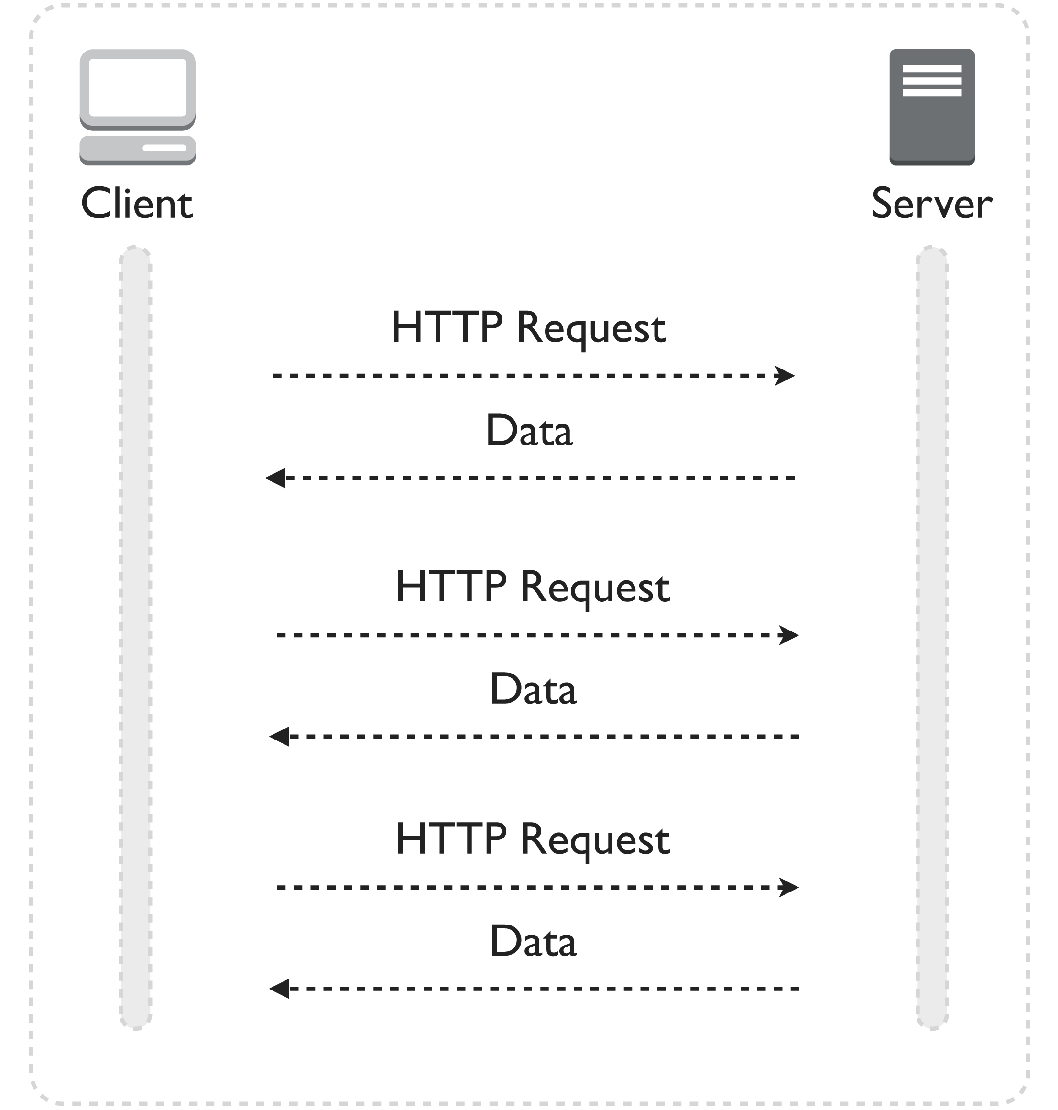
\includegraphics[width=1\textwidth]{images/client-server-http.pdf}
    \caption{A Client Fetches Data from A Server with HTTP}
    \label{fig:client-server-http}
  \end{center}
\end{figure}


However, this approach can radically improved by removing the redundant HTTP Requests. Then we transfer all data over a single TCP connection. This is what we called the WebSocket Protocol. We will expand more about the WebSocket Protocol in Subsection \ref{HTML5andWebSockets}.

\subsection{HTML5 and WebSockets}
\label{HTML5andWebSockets}

HTML5 is hypernym that consist of a large number of web technology \cite{wang2012definitive}. HTML5 covers the following area: new semantics, new CSS styling, multimedia, Graphics and 3D, Device Access, Performance, offline \& storage and connectivity. Amount all, the connectivity consists of communication technology such as Web Real-Time Communications (WebRTC), Server-Sent Events (SSE), Cross-Document messaging and WebSocket. WebRTC\footnote{http://www.webrtc.org/reference/architecture} provides realtime multimedia communication on web without requiring plugins; SSE provides an API for a browser to receive pushing notification from a server via an HTTP connection \cite{hickson2009server}; While Cross-Document messaging or Web Messaging largely expands the possibility and capability of communication of web browsers with least side-effect on security and privacy. Cross-Document messaging is designed to overcome the same-origin policy.

The goal of WebSocket technology is to provide a mechanism for browser-based applications that need two-way communication with servers that does not rely on opening multiple HTTP connections (e.g. using XMLHttpRequest or <iframe>s and long polling)\footnote{http://www.websocket.org}. Older web technology, like HTTP, remains inefficiencies problems \cite{wang2012definitive}. Firstly, it is not natively designed for nowadays Web Applications with rich contents and interactive demands; Secondly, overheads and unnecessary information cumulate swiftly as the interaction between the client and server continues. WebSocket improves communication problems by solving the above problems, while keeping simplicity. Both WebRTC and WebSocket are in effort to enhance the real-time communication. WebRTC provides APIs that allow web browsers communicate with each other directly, while WebSocket provides the real-time communication mechanism between a client and a server. Figure \ref{fig:client-server-ws} illustrates sequence diagram where a client (browser) fetches data from a server using WebSockets.

\begin{figure}[ht]
  \begin{center}
    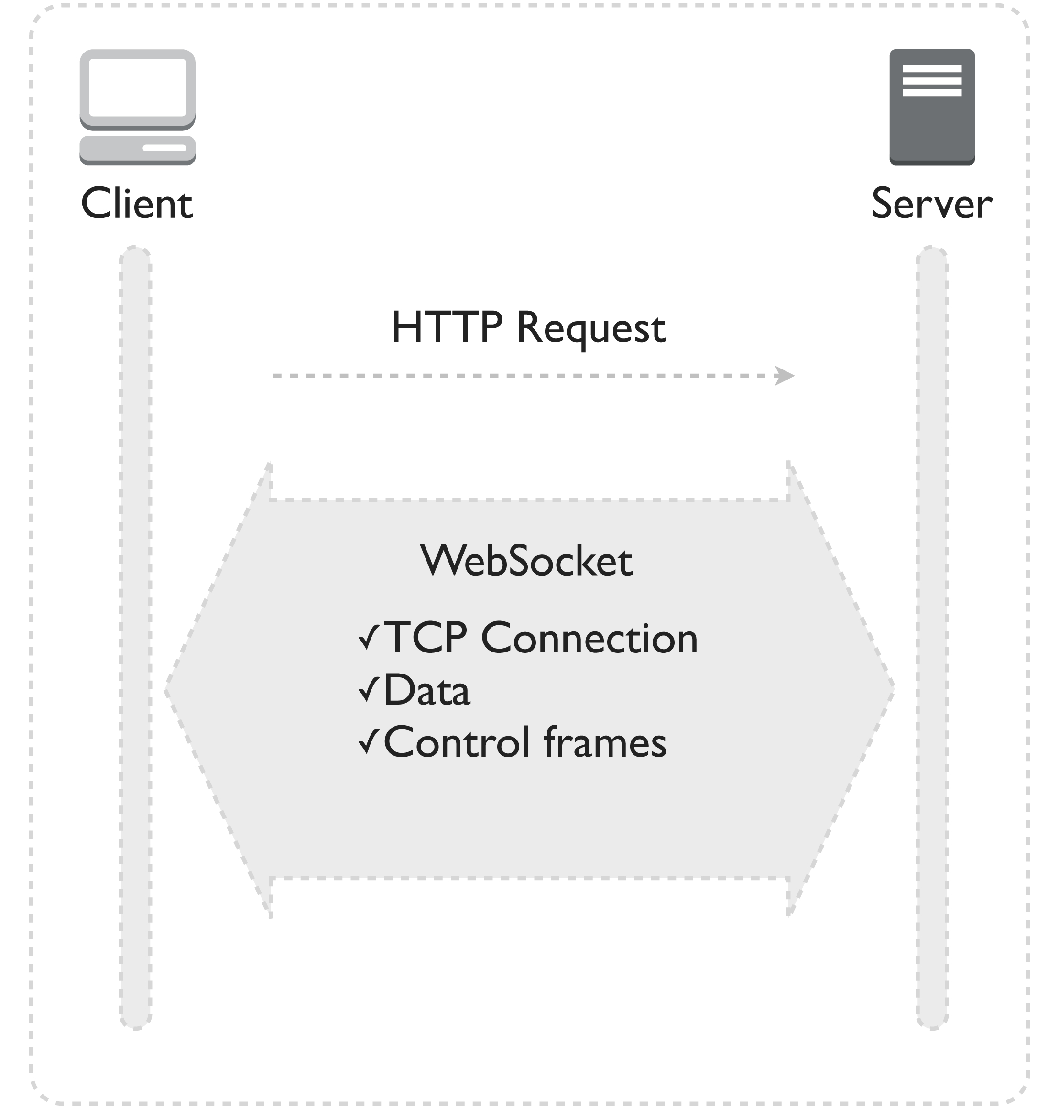
\includegraphics[width=1\textwidth]{images/client-server-ws.pdf}
    \caption{A Client Fetches Data from A Server with WebSockets}
    \label{fig:client-server-ws}
  \end{center}
\end{figure}

\section{Traditional Communication}

The client/server model is one of the network architectures to connect computers or applications, where the server provides resources and the client requests for the resources. Usually, the client/server model is designed as a request/response model, where the server does not actively communicate with clients. The client could be a computer, or an application, such as a web browser. The server is, usually, a (powerful) computer that keeps some applications running as constantly as possible. Those applications could be a database, a web server (application), or a printer server (application) that links to a physical printer. 

The HTTP protocol is a request/response protocol \cite{fielding1999hypertext}, where a client, or rather a user agent (UA) communicates with a server through a request and a response message(s). In other words, a client retrieves resources from a server in a request message, while the server hands over the contents in a response message. This is a general model that a client retrieves data from a server. 

Generally, there are three ways to retrieve data \cite{lubbers2010html5}: polling, long polling and streaming. All these approaches are uni-directional. 

With \emph{polling}, a client sends a request to a server, e.g. a web browser sends a request with Asynchronous JavaScript and XML (Ajax) \cite{garrett2005ajax} to a web server and expects data. This is an efficient solution, if the client knows exactly the time when the data is available. However, the server might not have the content when the client requests, or the content may be temporarily unavailable. If this situation would happen in practise, the client would have repeated polling for data. This will result in a large redundant headers generated by HTTP protocol, and a hight number of TCP connections. Consequently, the approach leads a heavy workload to the server and will not be suitable in the scenario, such as, some Internet scenarios with a large number of nodes. 

Another method, Long polling, is an improved approach, with respect to the frequency of request. Compared with polling, long polling does similarly, expect that the server holds the client's request for a certain period until timeout. Within this period, the server will send a response(s) back to the client, if there is data available. This method reduces the frequency of HTTP requests, but it increases the workload of a server, such as, ports handling. Generally, an HTTP request is initiated over TCP/IP connections (but any other protocols that guarantee a reliable transport can be used) \cite {fielding1999hypertext}. In TCP/IP connections, a port number is 16 bits \cite{postel2003rfc}, which means the maximum number of ports is \(  2^{16}  = 65536 \). However, one characteristic in the aforementioned Internet scenarios is scalability, which means the number of nodes could yield to a larger amount than that of the ports. Even though all ports are dedicated to communication, it is insufficient to support the schema with an enormous number of Internet-based nodes. 

As for the HTTP streaming, or known as HTTP server push, a server sends a response and keeps the connection open and alive, where the connection is triggered by a client's request. The drawback of this approach is that streaming is still encapsulated in HTTP, and thus buffer mechanism might increase the latency of messages delivering. Moreover, buffer is not an approach for an energy constrained device.

\section{WebSocket}

In the concept of Internet of Things (IoT), the networked objects, called devices, are deployed worldwide and connected over the internet. Moreover, the IoT device is individually addressable, so that each device is interconnected and can be accessed through the standards of the web. With the purpose of performing a better communication with IoT devices, the WebSocket protocol enables two-way communication and is arranged to substitute the disadvantage that existing in the traditional client/server model.

The WebSocket protocol supports data frame including text and binary. Once the WebSocket connection has been successfully established, generally, data frames transfer between a client and a server. However, in consideration of optimising WebSocket connections between a client and a server, the client can request that the server use a specific subprotocol by including the |Sec-WebSocket-Protocol| filed in its handshakes\cite{rfc64552012web}. A subprotocol is a application-level protocols layered over the WebSocket protocol\cite{rfc64552012web}. A subprotocol could be implemented by the servers and can be also versioned. The server chooses one or none subprotocol. 

\section{WAMP}

WebSocket Application Messaging Protocol (WAMP)\footnote{http://wamp.ws/} is a subprotocol officially registered in WebSocket Protocol Registries\footnote{http://www.iana.org/assignments/websocket/websocket.xml\#subprotocol-name} , which gives structure to messaging by providing two hight level messaging patterns: Publish/Subscribe (Pub/Sub) and Remote Procedure Calls (RPC).

WAMP fills in the blanks in the WebSocket protocol: a low-level specification which originally provides raw messaging communication (text or binary). Moreover, WAMP does not make any extra standard, but it bases on established Web standards: WebSocket, JSON and URI. The WebSocket standard is the default transport channel where WAMP is binding. With the WebSocket Standard, WAMP is assumed to be given a reliable, ordered, and full-duplex message channel. 

\section{Other Registered Subprotocols}

Apart from WAMP, there are MessageBroker WebSocket Subprotocol (MBWS), Simple Object Access Protocol (SOAP) and Simple Text Oriented Messaging Protocol (STOMP) can be used as subprotocols, according to the WebSocket Protocol Registries.

MBWS is used by messaging clients to send messages to, and received messages from, an Internet message broker. The Internet message broker is also called a message broker which queues messages, sent by clients, for asynchronous deliveries to clients \cite{hapner2012messagebroker}. Like WAMP, MBWS provides full-duplex and reliable transport; unlike WAMP, MBWS does not obviously provide higher level messaging patterns. MBWS, however, defines a binary message frame starting with an MBWS binary header, and a text message frame starting with an MBWS text header. MBWS provides two additional features. Firstly, it supports connection recovery, which has not defined by the WebSocket protocol. Secondly, it supports metadata in MBWS message headers. MBWS has a light weight version, called MessageBrokerLight WebSocket Subprotocol (MBLWS) which only supports Message Metadata \cite{hapner2012messagebroker}. However, MBWS is still a draft. 

SOAP is a lightweight protocol intending for exchanging structured information in a decentralised and distributed environment. SOAP uses XML technology to exchange data\cite{gudginsoap}. Microsoft, additionally, defines SOAP Over WebSocket Protocol Binding (MS-SWSB)\footnote{http://msdn.microsoft.com/en-us/library/hh536812.aspx}, a subprotocol for the WebSocket Protocol. The subprotocol involves a Web Services Description Language (WSDL) and supports message exchange patterns (MEPs). With MEPs, SOAP supports one-way, two-way and request/response message exchange patterns, which involves Pub/Sub and RPC.

Simple (or Streaming) Text Orientated Messaging Protocol (STOMP)\footnote{http://stomp.github.io} is a frame-based protocol. It refers to a STOMP frame includes a command, optional headers and a body. STOMP is text-based with UTF-8 encoding by default, but it, optionally, supports binary messages. As for message patterns, STOMP version 1.2 supports Pub/Sub. An example of Pub/Sub model using STOMP with WebSocket is discussed in \cite{wang2012definitive}.

Table \ref{table:subprotocol-comparison} is a comparison summary among WAMP, MBWS, SOAP and STOMP:

% If you need to have linefeeds (\\) inside a cell, you must create a new
% paragraph-formatting environment inside the cell. Most common ones are 
% the minipage-environment and the \parbox command (see LaTeX documentation
% for details; or just google for ``LaTeX minipage'' and ``LaTeX parbox'').
\begin{table}
\begin{tabular}{|p{2.2cm}|>{\centering\arraybackslash}p{2.2cm}|>{\centering\arraybackslash}p{3cm}|>{\centering\arraybackslash}p{1.5cm}|>{\centering\arraybackslash}p{2.9cm}|} 
% Alignment of sells: l=left, c=center, r=right. 
% If you want wrapping lines, use p{width} exact cell widths.
% If you want vertical lines between columns, write | above between the letters
% Horizontal lines are generated with the \hline command:
\hline % The line on top of the table
\textbf{ } & \textbf{WAMP} & \textbf{MBWS} & \textbf{SOAP} & \textbf{STOMP} \\ 
\hline 
% Place a & between the columns
% In the end of the line, use two backslashes \\ to break the line,
% then place a \hline to make a horizontal line below the row 
\textbf{Data Representation} & JSON & binary and text with MBWS headers & XML & binary and text with headers \\ 
\hline
\textbf{Message Patten} & Pub/Sub, RPC & not specified & MEP & Pub/Sub \\
% The multicolumn command takes the following 3 arguments: 
% the number of cells to merge, the cell formatting for the new cell, and the
% contents of the cell
\hline
\textbf{Connection Recovery} & no & yes & no & no \\
\hline
\textbf{Metadata} & currently no & yes & yes & no \\
\hline
\textbf{Released} & yes & draft & yes & yes \\
\hline
\end{tabular} % for really simple tables, you can just use tabular
% You can place the caption either below (like here) or above the table
\caption{WAMP and other WebSocket subprotocols}
\label{table:subprotocol-comparison}
\end{table} % table makes a floating object with a title


\chapter{Internet Of Things}
\label{chapter:internetofthings} 

\section{Things: Bridging The Real and The Virtual World}

The term, Internet of Things, was firstly mentioned by Kevin Ashton in once his presentation in 1999 \cite{ashton2009internet}.

Semantically, Internet of Things means ``a world-wide network of interconnected objects uniquely addressable, based on standard communication protocols'' \cite{infso2008networked}. 

The ``things'' refers to the ``objects'' in the semantical explanation. The ``things'' are heterogeneous objects. The initial idea of the ``things'' started with Radio-Frequency IDentification (RFID) tags by Auto-ID Labs\footnote{http://www.autoidlabs.org}, a world-wide network of academic research laboratory in the field of networked RFID and emerging sensing technologies. Hereafter, other concepts of ``things'' emerged: NFC tags, Wireless Sensor and Actuator Networks (WSANs), Spime and Smart Items.

\subsection{NFC and WSANs}

NFC is a proximity technology that provides contactless communication by using ISO/IEC 14443 and ISO/IEC 18092. NFC tags utilise Reader/Writer mode, one of the modes that a NFC devices should supports \cite{Madlmayr:SecurityandPrivacy}, to store data and interact with users. A typical scenario is that a NFC tag acts as a smart poster, where a user could place a NFC based mobile phone near a smart poster and thus would retrieve further information. For instance, if a smart poster stores movie poster data, it can forward a user to the movie trailer or its home page. Additionally, there are card emulation mode and Peer-to-Peer mode. Card Emulation Mode e.g. turns a mobile phone into a smart card such as a credit or debit card, and the NFC reader cannot distinguish the difference between the mobile phone and smart cards. Thus, with this features, it can implement a new way of payment system called Mobile Payments. NFC Peer-to-Peer (P2P) mode is designed based on the standards ISO 18092, which allows two NFC devices communicate mutually \cite{Madlmayr:SecurityandPrivacy}.

WSANs are composed of large numbers of minimal capacity sensing, computing, and communicating devices and various types of actuators. WSANs constitute an important and exciting new technology with great potential for improving many current applications. It also creates new revolutionary systems in areas such as global-scale environmental monitoring, precision agriculture, home and assisted living medical care, smart buildings and cities, industrial automation, and numerous military applications \cite{stankovic2008sensor}. 

They are, together with RFID, are recognised as the atomic components that links the real world with the digital world \cite{sterling2005shaping}.

\subsection{Spime and Smart Items}

Spime and Smart Items are also considered to be the ``things''. Spime is a neologism created by Bruce Sterling, a science fiction writer, in 2005. Sterling stated that there will be a new kind of object -- user-alterable, baroquely multi-featured and programmable -- in the future, for which Sterling invented the term ``Spime'' \cite{sterling2005shaping}. Sterling described that the Spime is one of the objects in Internet of Things since Spime enables a thing to be searchable. i.e., A thing can be searched by a search engine from a virtual world to a physical world \cite{sterling2005shaping}. Spime is a bit theoretical, but we can find some of its prototype in the real world, and we call them Smart Items \cite{atzori2010internet}.

IoT is also derivative from the vision of ``Internet'', which Vasseur and Adam described in \cite{vasseur2010interconnecting}. A Smart Object is an item equipped with a form of sensor or actuator, a tiny microprocessor, a communication device and a power source. The sensor or actuator gives the smart object the ability to interact with the physical world. Smart Objects are interconnected using the Internet Protocol (IP). 

According to IPSO Alliance, the IP stack is a light protocol that already connects a huge amount of communicating devices and runs on tiny and battery operated embedded devices. This guarantees that IP has all the qualities to make IoT a reality \cite{atzori2010internet}.

\section{Sensors and Actuators}
A sensor detects or measures the physical environment (such as temperature, speed, and location etc) and converts it to a form (such as a digital form) which can be read by human or used for other purpose. For example, a light sensor senses the brightness of the environment, then the sensor converts the brightness into a digital form (data). The data can be, further, transferred to other receivers.

Sensors can interconnect wirelessly, and form a network, which is called wireless sensor network (WSN). WSN monitors the environment or other physical data distributively. According to \cite{culler2004guest}, WSN can be apply to a wide range of uses: monitoring space, things, and the encompassing space. Particularly, the first category, space, which is related to the thesis, covers light, temperature, humidity and other environment data. 

Sensors perform tasks more than measuring environments. The second category applies on things or objects. Sensors, that being the case, are applied more in area of such as, the detection of structures breakages \cite{christin2009wireless}. However, things and the environment are sometimes interconnected and interactive. This is the third category when sensors are used to e.g. monitor the wildlife habitats \cite{culler2004guest} and the interaction between traffic queuing and the frequency of traffic lights switching. In short, the WSN provides a good source of data for Internet of Things.

Sensors collect and transfer data for further use, but an actuator provides controlling functions to a system. e.g. a light switch can turn on and turn off a light; Here the light switch is an actuator. Sensors and Actuators work mutually can optimise processes. For example, sensors are installed in chemical production to bring much greater granularity to monitoring, where the sensor collects data and transfers them to computers which subsequently analyse the data and signal actuators to adjust the processes, such as ingredient mixtures, temperatures, or pressures \cite{chui2010internet}. The whole process can then be automated. 

\section{Internet-based Communication Protocols}
The currently architecture of IoT consists three layers \cite{wu2010research}. From top to bottom, they are: application layer, network layer and perception layer. The perception layer consists of the unquietly addressable objects. The network layer connects the objects and connects objects to computers. The application layer makes the IoT data meaningful, useful or extensible.

TCP/IP and UDP ensure the objects communicable in IoT. Moreover, they ensure that the objects can be communicated outside the IoT network. Subsequently, the data collected by sensors are usable. For example, the data collected by sensors can be transferred to a data centre and can be further analysed. 

Another issue about IP, Internet Protocol Version 4 (IPv4) is the dominant IP protocol in the Internet currently. IPv4, however, has exhausted \cite{smith2011free} and thus could not meet the `unquietly addressable' requirement in IoT. IP Version 6 (IPv6) is its successor. ``IPv6 enables end-to-end communication, in which any IPv6 `smart things' can connect to any other IPv6 devices or system from any place and at any time. It enables the possible extension of the Internet to any device, sensor or actuator, which can become real nodes of the future Internet.'' \cite{vermesan2011internet}. It primarily provides the following features \cite{deering1998internet}: 

\begin{itemize}
% You can use this command to set the items in the list closer to each other
% (ITEM SEParation, the vertical space between the list items) 
\setlength{\itemsep}{0pt}
\item Expanding addressing capabilities to support a greater amount of addressable nodes. 
\item Simplifying header format to reduce the cost of packet handling.
\item Improving support for extensions and options to allow greater flexibility in the future.
\item Flowing labelling capability to label packets and thus to handle, e.g., real-time services.
\item Authentication and privacy capabilities.
\end{itemize}

HTTP and WebSocket ensure that IoT can be used or extended by applications. For example, a web interface that can visualise temperature data. Subsequently, IoT network can be directly or indirectly connect to end users. 

A Web Service ``is a network accessible interface to application functionality, built using standard Internet technologies'' \cite{snell2009programming}. In other words, an application can be accessed by another application, client or user over the Internet, via web technology such as HTTP, XML or SMTP. A Web Service, usually, provides services based on standards at the layer between service requesters and service providers. This means, it does not matter how are the services implemented, e.g. using C/C++, Java, Python or Javascript, or based on whatever platforms, e.g. Windows, Max OS or Unix. 

When a request is sent to a web service layer, this layer will start a procedure which further requests the service provider. When the procedure is finished, the web service layer will response to the sender results (the response is sometimes optional and it relies on how is the web service implemented). The communication, between the service requesters and the web service layer, is usually based on standard protocols, which aims at cross-platform interoperability. 

In the following, we will talk about a sequence of protocols that can be used in Web Services.

\subsection{REST}
Representational State Transfer (REST) is introduced by Roy T. Fielding in his doctoral dissertation in 2000 \cite {fielding2002principled}. REST is a web architectural style. It is, however, not a standard or protocol. 

An architectural style is ``a coordinated set of architectural constraints that restricts the roles and features of architectural elements, and the allowed relationships among those elements, within any architecture that conforms to the style. Thus, a style provides a name by which we can refer to a packaged set of architectural design decisions and the set of architectural properties that are induced by applying the style.'' \cite {fielding2002principled}

REST was developed in parallel with HTTP protocols with the basic four constraints: resources identified by URI; resources manipulated by standard HTTP methods; resources with various representations; and stateless communication. Resources are data that can be addressed by URIs, which further implies resources are differed by URIs. A representation is a way to present resources. For example, a text, an Image or an HTML document. The representation, moreover, consists of metadata describing the data and, occasionally, metadata describing metadata.

All REST communications are stateless. Thus, each request involves all the necessary information that a receiver needs to understand the request. An example of stateless design is shown in Figure \ref{fig:stateless-design} \cite{rodriguez2008restful}

\begin{figure}[ht]
  \begin{center}
    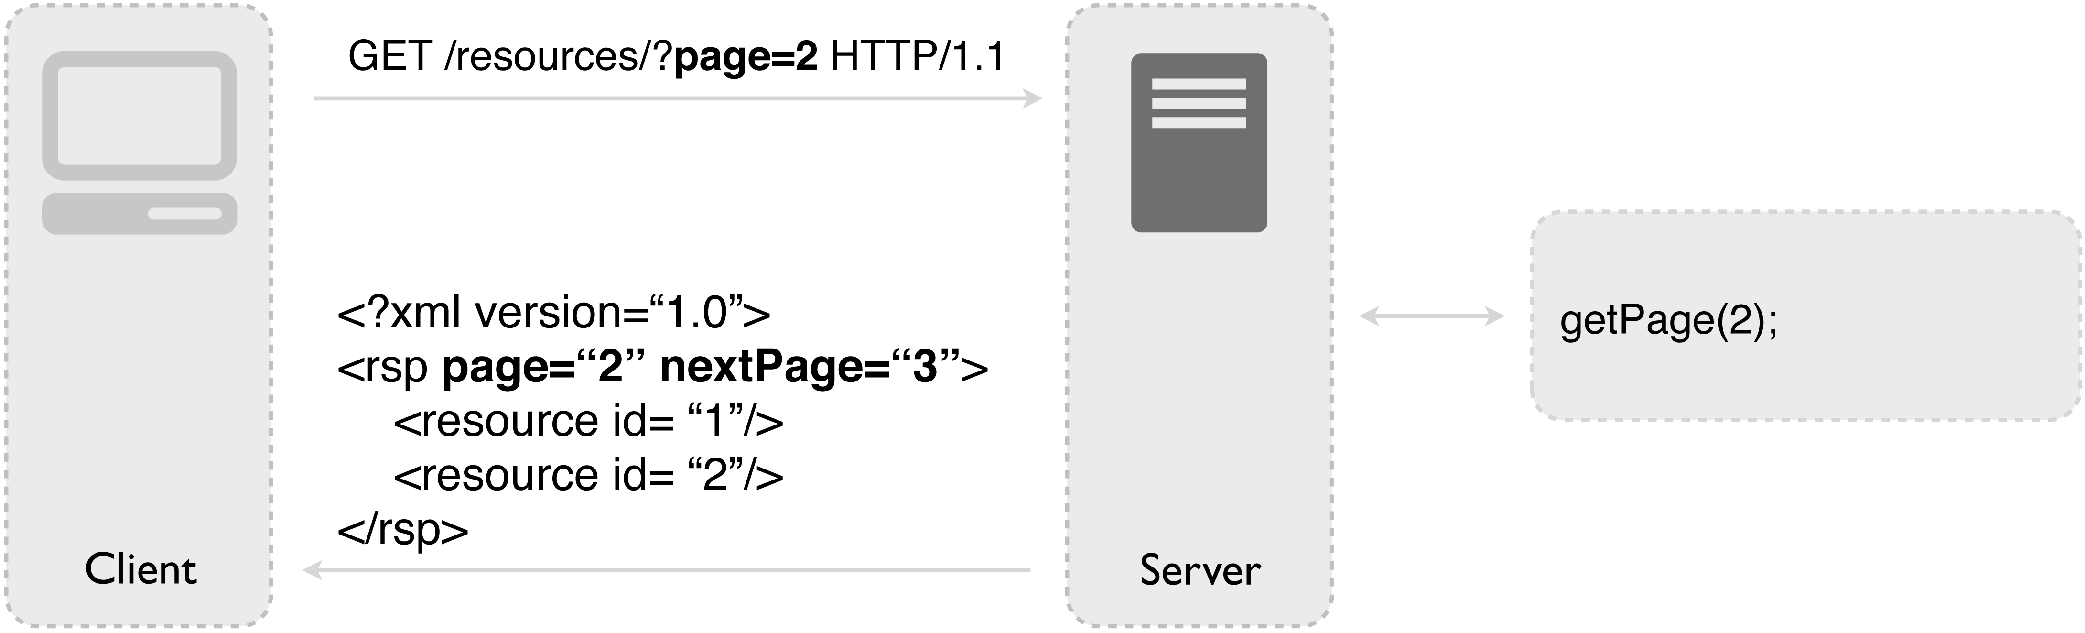
\includegraphics[width=1\textwidth]{images/stateless-design.pdf}
    \caption{Stateless Design}
    \label{fig:stateless-design}
  \end{center}
\end{figure}

As it is illustrated, the request specifies which page the client fetches, i.e., page 2; while the response message contains what the current page is, what the next page is and also the requested page.

On the contrary, stateful design, as shown by Figure \ref{fig:stateful-design} \cite{rodriguez2008restful}, the server saves each client status and responses the corresponding status to the clients who request them. In \ref{fig:stateful-design}, the client need not to specify which page it fetches, but just call the corresponding procedure. The server computes the result and returns the page to the client.

\begin{figure}[ht]
  \begin{center}
    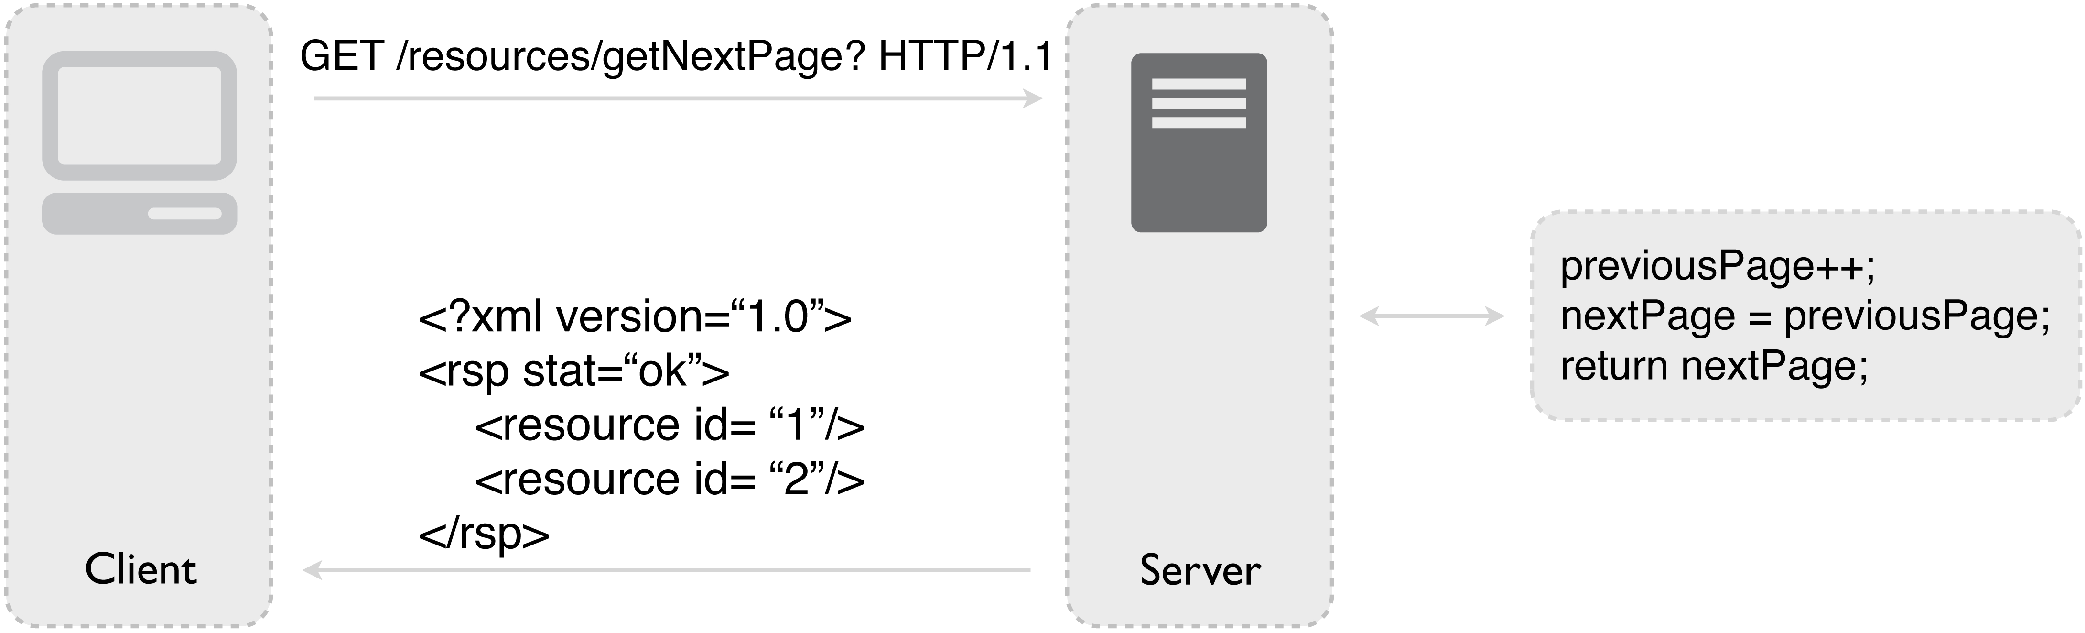
\includegraphics[width=1\textwidth]{images/stateful-design.pdf}
    \caption{Stateful Design}
    \label{fig:stateful-design}
  \end{center}
\end{figure}

The replies are in XML format in Figure \ref{fig:stateless-design} and \ref{fig:stateful-design}, but the REST reply is not restricted in XML document. It could be JSON or other data structure. Usually, REST is implemented relying on HTTP and other web technologies. 

\subsection{SOAP}
SOAP, a protocol designed for web services, specifies, firstly, a XML-based envelope to transfer information; Secondly, a set of rules for translating application and platform-specific data types into XML representations \cite{snell2009programming}. 

SOAP is largely based on XML standards and provides a standard way to structure XML messages. Thus, SOAP has two related applications: Remote Procedure Call (RPC) and Electronic Document Interchange (EDI). RPC is one way to do distributed computing, where one programme calls a function or method (called procedure) on another, optionally with parameters and receiving return value. EDI is used in automated transactions.

A SOAP message contains an optional SOAP header and a required SOAP body. The SOAP header consists of several information blocks and each of the block is a header. Each header explains how the message is to be parsed. The message body is the actual message in XML syntax. 

SOAP provides a mechanism to handle errors which is called SOAP Faults. A SOAP fault consists of fault code, fault string, the fault actor and the fault details. The fault code has been standardised in namespace belong to \url{http://www.w3.org/2001/06/soap-envelope}; The fault string is an explanation of the error for human to read, while the fault detail is a further explanation about the error. The actor is a concept in SOAP Message Exchange Patterns (MEP), a pattern of message exchanged between SOAP nodes, which has been standardised at \cite{booth2007web}.

When a SOAP message is sent from a provider to a receiver, it passes one or more web services. Each of the web service is called intermediary. All these intermediaries that the SOAP message travels through is called a message path. We call each intermediary on a message path an actor. Thus, the fault actor is the unique identifier of message processing node where the error occurs. 

SOAP does not specify the means of SOAP message transports. Generally, SOAP can be transferred through HTTP, FTP, BSD sockets and SMTP etc. 

\subsection{CoAP}
Constrained RESTful Environments (CORE) is a working group under Internet Engineering Task Force (IETF) foaming in 2010\footnote{https://datatracker.ietf.org/wg/core/history/}. CORE has been contributing the major standardisation work for Constrained Application Protocol (CoAP). 

CoAP is a protocol (in draft) used in constrained nodes and constrained networks and designed for machine-to-machine (M2M) applications \cite{shelby2013constrained}. A constrained node, usually, has a lower capacity controller with a small amount of ROM and RAM. Constrained networks refer to the networks, generally, with high packets error rates and a low throughput.

CoAP applications or endpoints interact via a request/response model. It also supports built-in services and resources discoveries. With CoAP, applications or endpoints can easily interact with an HTTP based web architecture \cite{shelby2013constrained}.

Unlike HTTP, CoAP stack is designed for constrained environment, while CoAP, additionally, differ from HTTP in terms of power consumption and overhead. Generally, CoAP power consumption bytes per-transaction are lower than those of HTTP, which implies longer battery lifetime. Figure \ref{fig:http-and-coap-stack} illustrates a comparison between HTTP and CoAP stack. CoAP consists of the concept of HTTP, but it has been re-designed with the respect to the low processing power and energy consumption constraints \cite{colitti2011integrating}.

\begin{figure}[ht]
  \begin{center}
    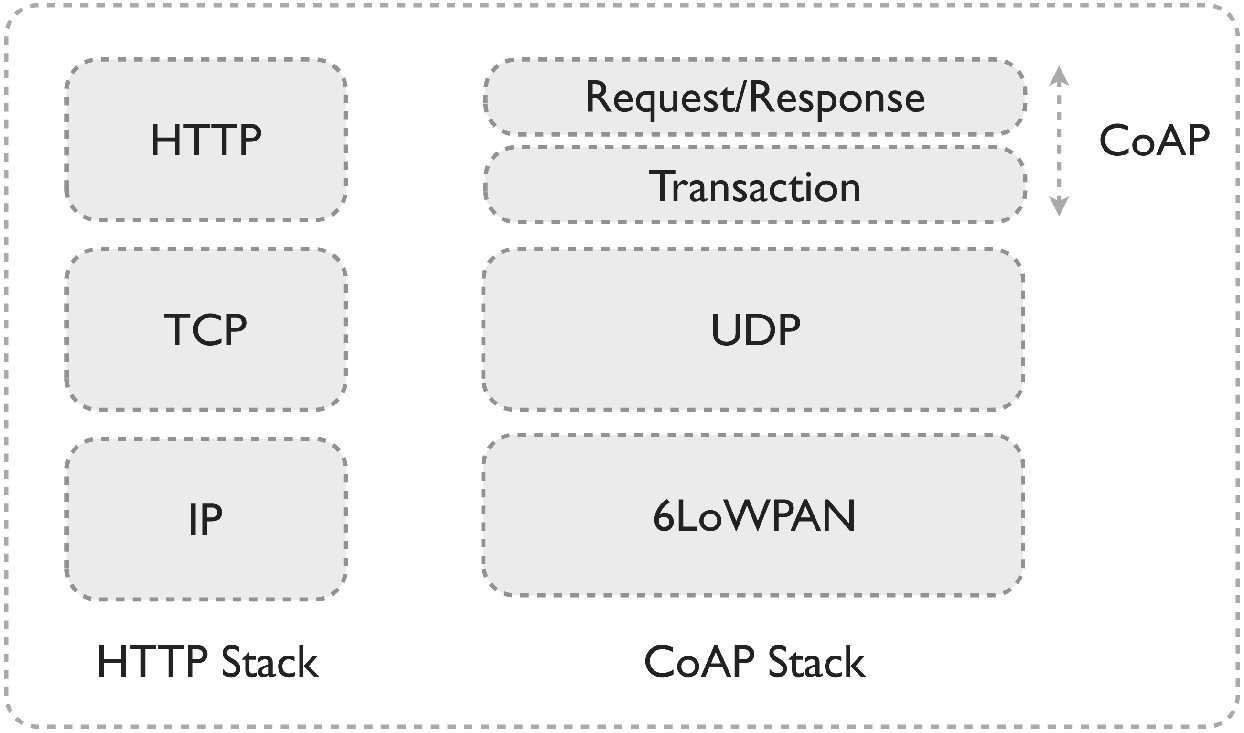
\includegraphics[width=1\textwidth]{images/http-and-coap-stack.pdf}
    \caption{HTTP and CoAP Stack Comparison}
    \label{fig:http-and-coap-stack}
  \end{center}
\end{figure}

CoAP relies on UDP. Moreover, CoAP cannot communicate with a browser directly without a gateway which translates CoAP to HTTP. The gateway can be an application. e.g. Copper\footnote{https://addons.mozilla.org/de/firefox/addon/copper-270430/}, a firefox plug-in, currently, is available for users to browse and interact with Internet of Things devices.

\subsection{MQTT}
Message Queuing Telemetry Transport (MQTT)\footnote{http://mqtt.org} is a machine-to-machine (M2M) / IoT connectivity protocol. There are two main specification for MQTT: MQTT v3.1 and MQTT-S (MQTT for Sensor) v1.2. We will compare MQTT V3.1 with WAMP. Since MQTT-S does not work on TCP/IP network, it is not suitable for the IoT thus will not be further discussed.

MQTT is designed as an extremely lightweight publish/subscribe messaging transport; while MQTT-S is a publish/subscribe messaging protocol for wireless sensor networks (WSNs) and is originally designed for non-TCP/IP networks.

MQTT V3.1 and WAMP are both working on TCP/IP network. Different from WAMP, MQTT V3.1 assumes the communications channel is more likely to be unreliable.

MQTT V3.1 has a two bytes message header and a UTF8 encoded payload.
Message type, such as Pub/Sub, is defined in the header. Unlike WAMP, MQTT V3.1 does not yet support RPC. Additionally, MQTT V3.1 provides three levels of Quality of Services (QoS) control.

Level 0 is called ``At most once delivery'', when the message is delivered highly dependent to the underlying TCP/IP network. There is no any expectation that the recipient will sent back a response and the message arrives at the recipient at once or it just loses.

Level 1 is called ``At least once delivery'', when a response is expected to be sent back from the recipient, otherwise, the sender will re-send the message.

Level 2 is called ``Exactly once delivery'', when the message will be received and only received once by the recipient. More helper messages will be exchanged at this level to ensure the quality of delivery, and hence there is an increase in the network traffic \cite{MQTTV31ProtocolSpec}.

WAMP, however, does not support such QoS control. Finally, WAMP has been officially registered in the WebSocket Subprotocol Name Registry, while MQTT is not a member.

\subsection{Comparison}
Table \ref{table:WAMPCoAPandMQTTcomparison} is a summary of the comparison between WAMP, CoAP and MQTT.

% If you need to have linefeeds (\\) inside a cell, you must create a new
% paragraph-formatting environment inside the cell. Most common ones are 
% the minipage-environment and the \parbox command (see LaTeX documentation
% for details; or just google for ``LaTeX minipage'' and ``LaTeX parbox'').
\begin{table}
\begin{tabular}{|p{3.3cm}|>{\centering\arraybackslash}p{3cm}|>{\centering\arraybackslash}p{3cm}|>{\centering\arraybackslash}p{3.3cm}|} 
% Alignment of sells: l=left, c=center, r=right. 
% If you want wrapping lines, use p{width} exact cell widths.
% If you want vertical lines between columns, write | above between the letters
% Horizontal lines are generated with the \hline command:
\hline % The line on top of the table
\textbf{ } & \textbf{WAMP} & \textbf{CoAP} & \textbf{MQTT} \\ 
\hline 
% Place a & between the columns
% In the end of the line, use two backslashes \\ to break the line,
% then place a \hline to make a horizontal line below the row 
\textbf{Transport Layer} & TCP & UDP & TCP \\ 
\hline
\textbf{Get Resource} & over WebSockets & HTTP Requests & BSD Sockets \\
% The multicolumn command takes the following 3 arguments: 
% the number of cells to merge, the cell formatting for the new cell, and the
% contents of the cell
\hline
\textbf{Browser} & yes, HTML5 support & no, only via Firefox plugin currently & no, not directly \\
\hline
\textbf{Server} & WebSocket Server with WAMP support & CoAP Server & MQTT Server \\
\hline
\textbf{RPC} & yes & request/response model (through REST APIs) & no \\
\hline
\textbf{Pub/Sub} & yes & yes & yes \\
\hline
\textbf{Proxy Support} & through WebSockets & built-in & external proxy to translate protocol (implies delay) \\
\hline
\end{tabular} % for really simple tables, you can just use tabular
% You can place the caption either below (like here) or above the table
\caption{WAMP, CoAP and MQTT comparison}
\label{table:WAMPCoAPandMQTTcomparison}
\end{table} % table makes a floating object with a title

 
\chapter{Design and Implementation of Web-based IoT Applications}
\label{chapter:Design-and-Implementation-of-Web-based-IoT-Applications}

\section{Patterns for Web-based IoT Applications}
\label{chapter:Patternsforweb-basedIoTapplications}

\subsection{RPC}
Remote Procedure Call (RPC) is one of the Inter-Process Communication methods for data exchange among threads or processes on different hosts. Unlike a local application case \cite{srinivasan1995rpc}, where the code runs all locally, RPC solves the problem of excusing codes of the whole application which is distributed cross different networks or the Internet.

RPC can be further developed into a massage pattern \footnote{http://wamp.ws/faq\#rpc} involving two roles, client and server. Usually, RPC pattern is initiated by a client, which sends an request to a remote server; The server processes based on the request, then responses to the client. An example of RPC pattern is shown in Figure \ref{fig:RPC-pattern}. The client starts its procedure sequence when the programme is running. The procedure sequence starts with Procedure 1. The client, afterwards, needs the result from Procedure 2 which locates on the Server. Thus, it sends a request to the server. The server handles the logic when the request comes, and thus it starts Procedure 2. At the moment, the Client is waiting for the result until the server responses to the client. With the result, the client can now continue to execute the next procedure, Procedure 3.  

\begin{figure}[ht]
  \begin{center}
    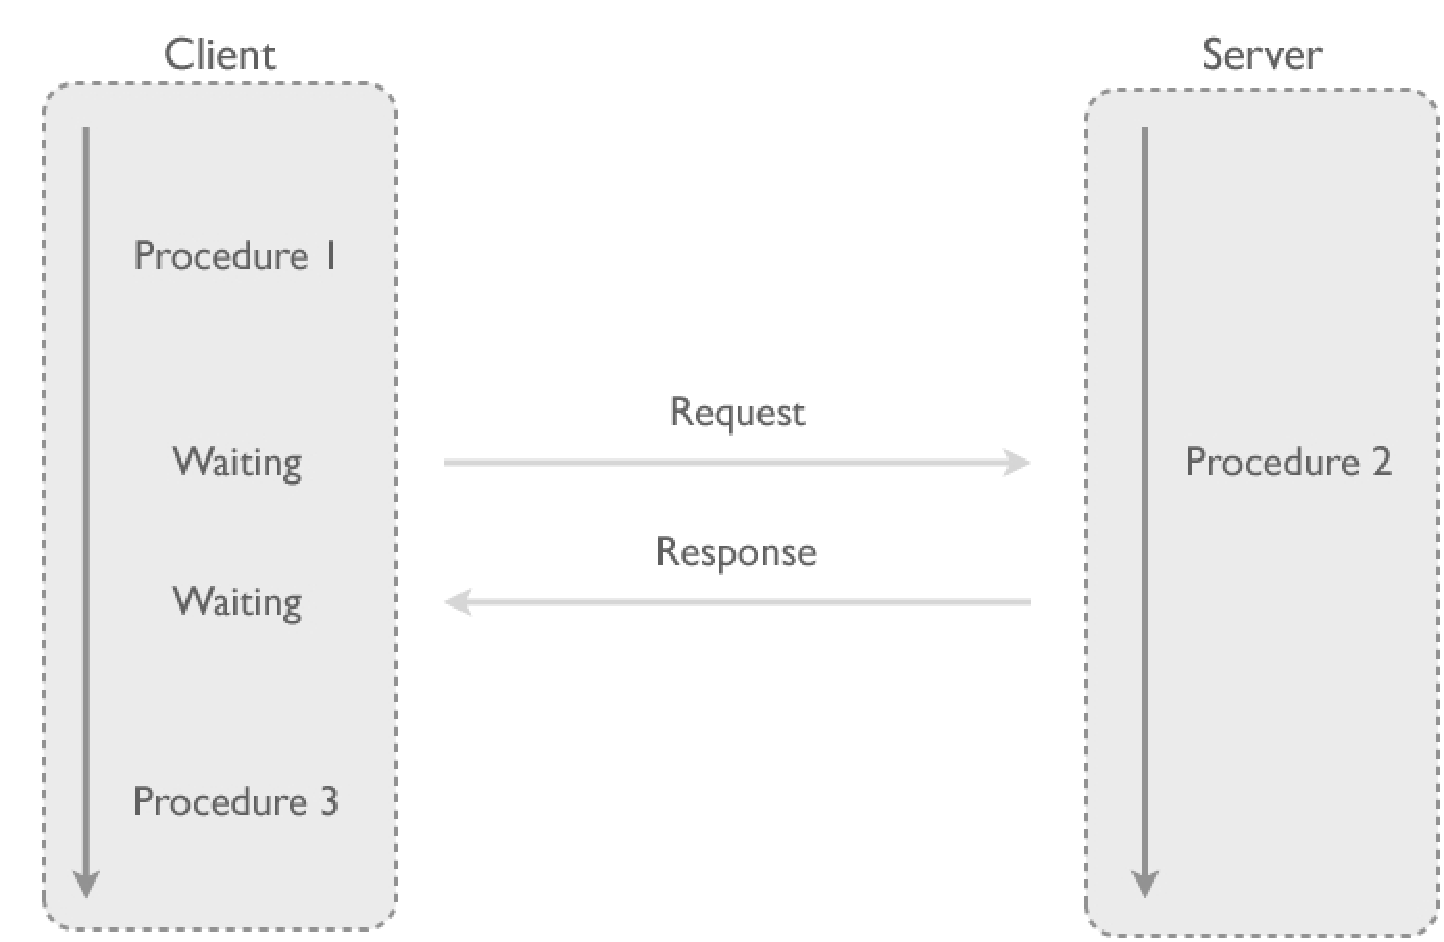
\includegraphics[width=1\textwidth]{images/RPC-pattern.pdf}
    \caption{An Example of RPC Pattern}
    \label{fig:RPC-pattern}
  \end{center}
\end{figure}

RPC is commonly used in real world scenarios. For example, Facebook, a social network web platform, provides open APIs that allows third party applications to access its data. Here, Facebook plays the role of the server(s), while the third party applications play the role of the client. When a third party application (client) sends a request to Facebook asking, e.g. a list of the user's friends, Facebook servers process the request. Facebook servers, then, response to the client, when the result, either success or error, is ready. The client can then use the list of friends to perform further procedures. 

From the perspective of IoT, RPC pattern covers one of the two most important interaction in the IoT application architecture, i.e. commanding. In the case of IoT, nodes could locate on different locations from cities to countrysides. Commanding is helpful to configure a node remotely, e.g. setting the parameters (device identification, timeout and reporting rate). As for an actuator, RPC pattern can control its action. e.g. a light actuator, or called a light switch, has the actions of on and off. With commanding, the light can, thus, be switched on or off remotely.

\subsection{Publish/Subscribe}

Publish/Subscribe (Pub/Sub) is one of the messages exchanges patterns. Messages are exchanged based on publishing and subscribing. A sender of a message is called a publisher. Usually, each message contains a topic. A receiver filters and receives a message by the message topic. The receiver who subscribes topics is called a subscriber. 

Pub/Sub architecture consists, usually, at least publishers, subscribers and a broker(s). The broker maps the right messages to the right receivers and exchanges messages among publishers and subscribers. Generally, there is, on one hand, no restricted boundary between a publisher and a subscriber. This means, a publisher can also be a subscriber and receives messages from other publishers; while a subscriber can also be a publisher and publishes messages with topics. On the other hand, there is no order between publishing and subscribing. This means, a publisher can publish a message with a topic without subscribing any topic; or even no one subscribes the topic. The subscriber does not have to subscribe any topic either. This refers to, if the aforementioned situation happens, then messages are , e.g., simply discarded. All the message exchanging logics, however, are handled by the broker(s). The broker(s) should specifies and implements corresponding functions to different messaging situations. 

An example of Pub/Sub pattern is shown in Figure \ref{fig:publish-subscribe-pattern}. Client 1 plays roles in both subscriber and publisher in different stages. i.e. When it subscribes topic 1, client 1 is treated as a subscriber. Client 1, however, changes to a publisher when it publishes a message with the topic (topic 1). The broker analyses the message and maps the topic to the subscribers who are interested in the topics. In this case, both Client 1 and Client 2 are interested in the topic. Hence, the broker replies the message to both of them. Client 1, and thus, changes its role to a subscriber.

\begin{figure}[ht]
  \begin{center}
    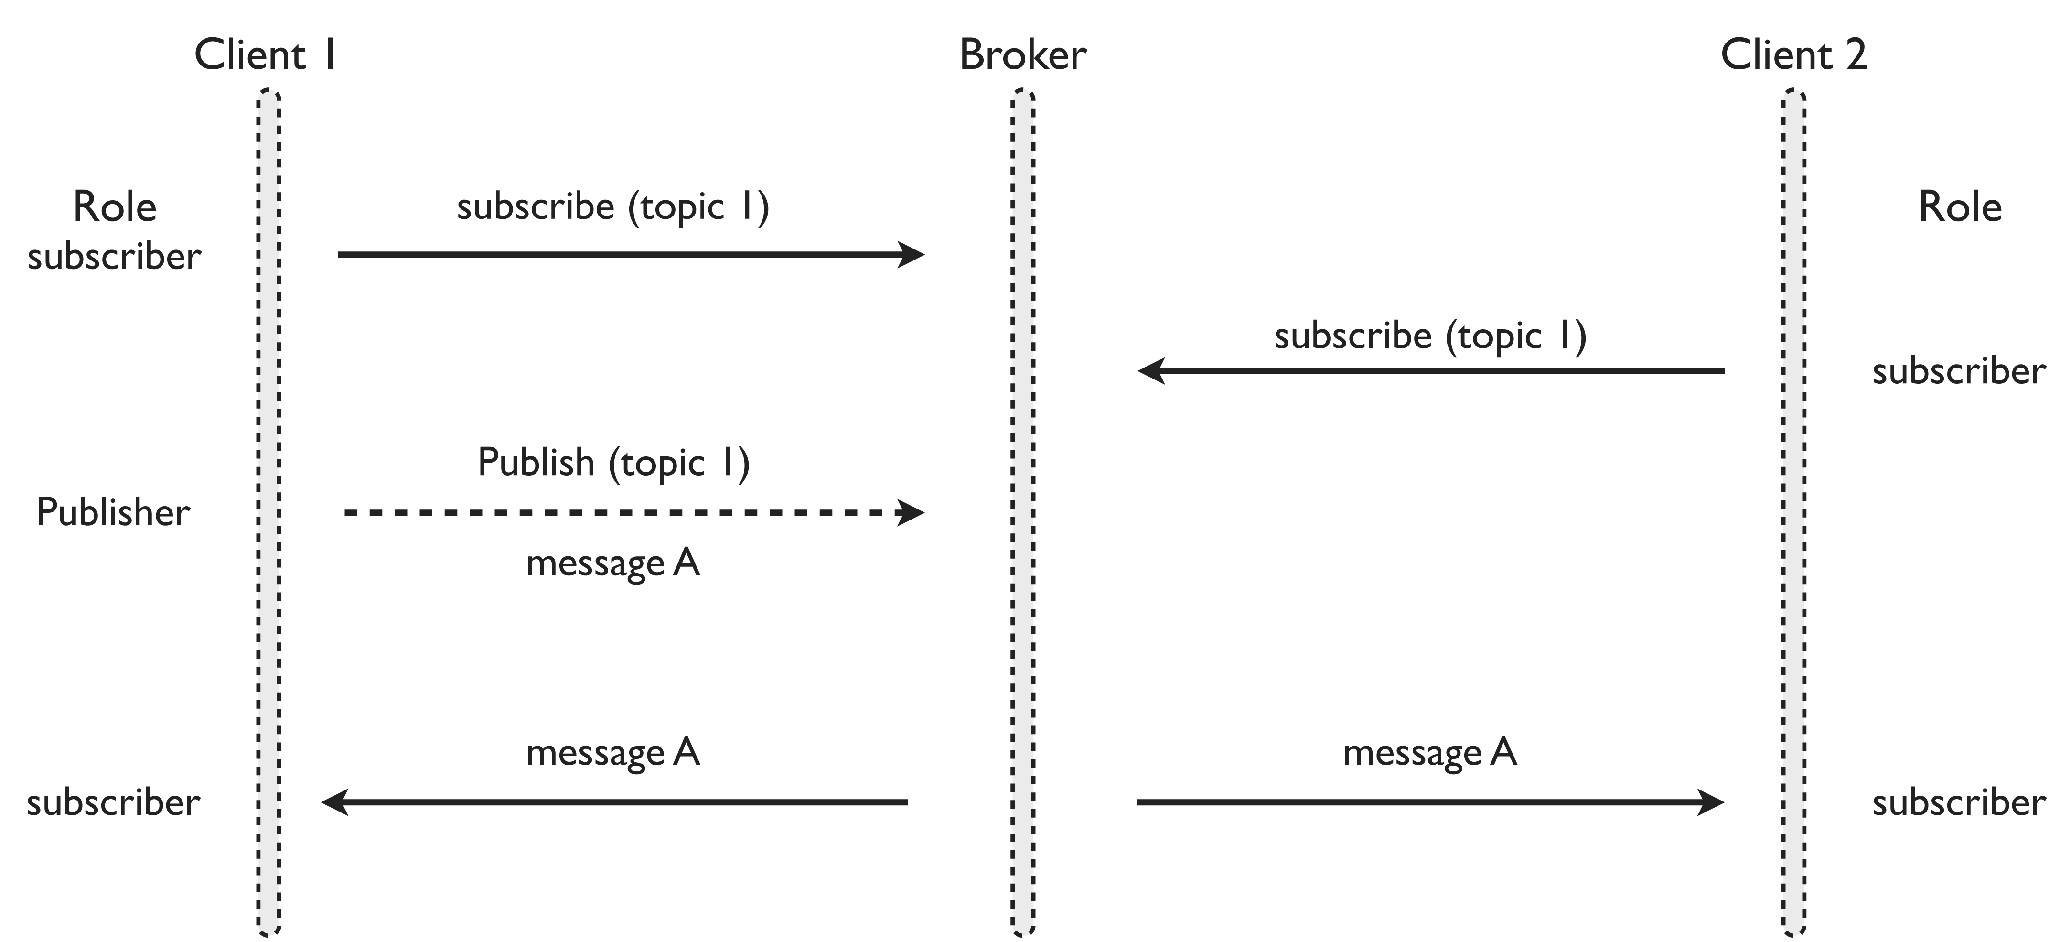
\includegraphics[width=1\textwidth]{images/publish-subscribe-pattern.pdf}
    \caption{An Example of Publish/Subscribe Pattern}
    \label{fig:publish-subscribe-pattern}
  \end{center}
\end{figure}

The concept of Pub/Sub pattern has been used in real world cases. Twitter, for example, can be treated as a real world scenario, even though the implementation might be different in Twitter. When a new user, User 1, posts a message in Twitter, usually, it will not popup on any other users' home page, but it will popup on User 1's homepage or a similar page that represents the user. This can be understood that User 1 subscribes himself, but no one subscribes him. 

User 1 can follow other users based on his interest. For example, User 1 follows User 2. User 1 will, then, receives User 2's post on User 1's homepage. Here, User 2 becomes a topic that User 1 subscribes; User 1 is the subscriber and User 2 is the publisher. Twitter, acts as a broker, handles the logic how the messages sent by User 2 delivers to User 1.

From the perspective of IoT, Pub/Sub pattern covers the other one of the two most important interaction in the IoT application architecture, i.e. notification. With notification, data can be sent interconnected, such as among nodes or from nodes to data centres. For example, one node, Node A, collects temperature data and humidity data. Node A then submits the collected data to the other node or data centre (called Node B) for the purpose of assembling. One strategy, which organises and manages the data sent by Node A, is to set the topic of the each message to the data type (i.e. temperature or humidity). Subsequently, Node B can easily categorise the data for further processing. There are, surely, other ways of exploiting Pub/Sub pattern. 

\subsection{Database-centric Approach}
Database-centric is a software architecture where database plays critical role. Generally, database provides fault tolerant and reliable transactions. Database-centric Approach, in IoT services, subsequently, provides a dependable mechanism to record enormous IoT data. 

An example of implementing a database-centric IoT service has been discussed in \cite{francesco2012storage}. The approach merges the features of database-centric approach with the demands of IoT services, and provides customised features for IoT services. Thus, the approach, firstly, supports heterogeneous and multimedia contents; Secondly, it provides standard APIs for standard web services, and thus the IoT data can be utilised at optimally maximum; Finally, live notification is supported and security features are applied.

\section{Smart Lighting and Control Application}
\subsection{Components}
In the thesis, we built an HTML5 based application to demonstrate a smart lighting and controlling IoT service. The concept of the sample service consists the following elements: a light, a switch, a sensor and the sun. The light is a component that visualises the light status. The switch is a component that represents an actuator that can control the light. The sensor is a component that senses the environment brightness. The sun represents the environment. The change of the luminance from the sun affects on the sensor which then affects on the light. The luminance of the light will be, subsequently, adjusted. The service allows the light to keep the brightness of a space constantly, or to be adjusted by the switch: on, off or to dim. The relationship among the components is shown in Figure \ref{fig:components-relationship}. 

\begin{figure}[ht]
  \begin{center}
    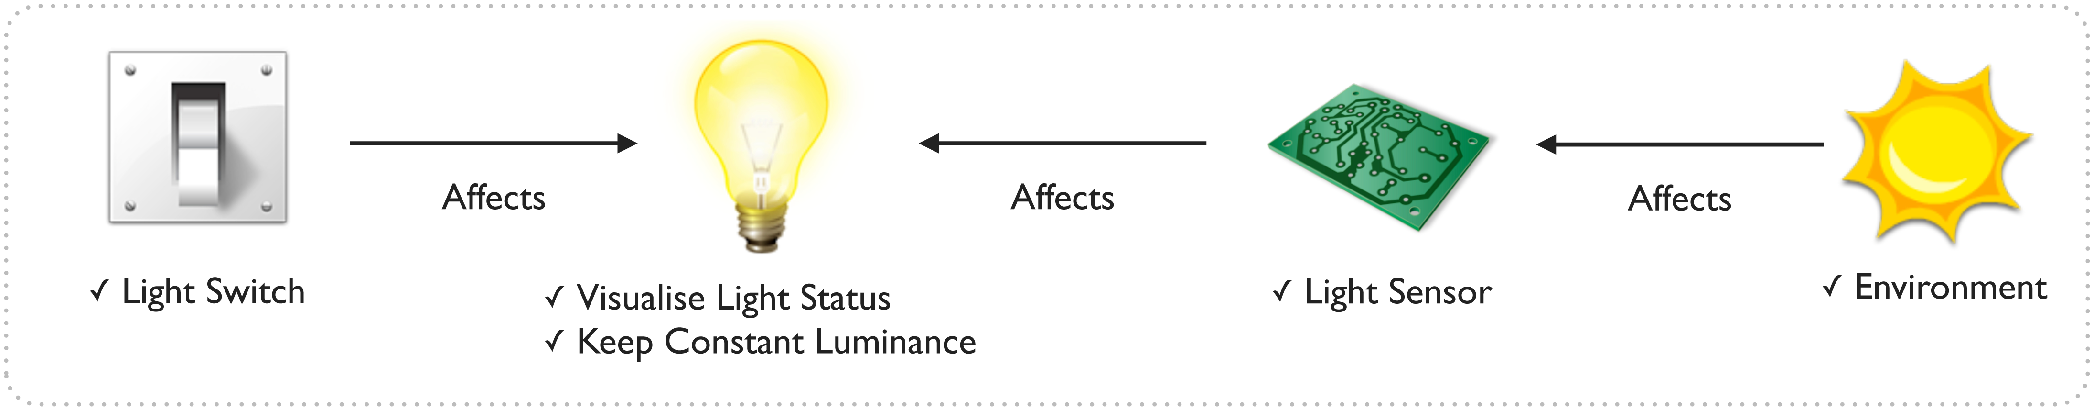
\includegraphics[width=1\textwidth]{images/components-relationship.pdf}
    \caption{Components Relationship}
    \label{fig:components-relationship}
  \end{center}
\end{figure}

\subsection{Implementation of The Backend}
With the concept above, we implemented an embedded web server based on a NodeJS server. We also attached a WebSocket server to the NodeJS server, and a WAMP server on top of the WebSocket server. The embedded web server, then, understands the WebSocket protocol and the WAMP subprotocol. The component layer structure is shown in Figure  \ref{fig:component-layer-structure}. 

\begin{figure}[ht]
  \begin{center}
    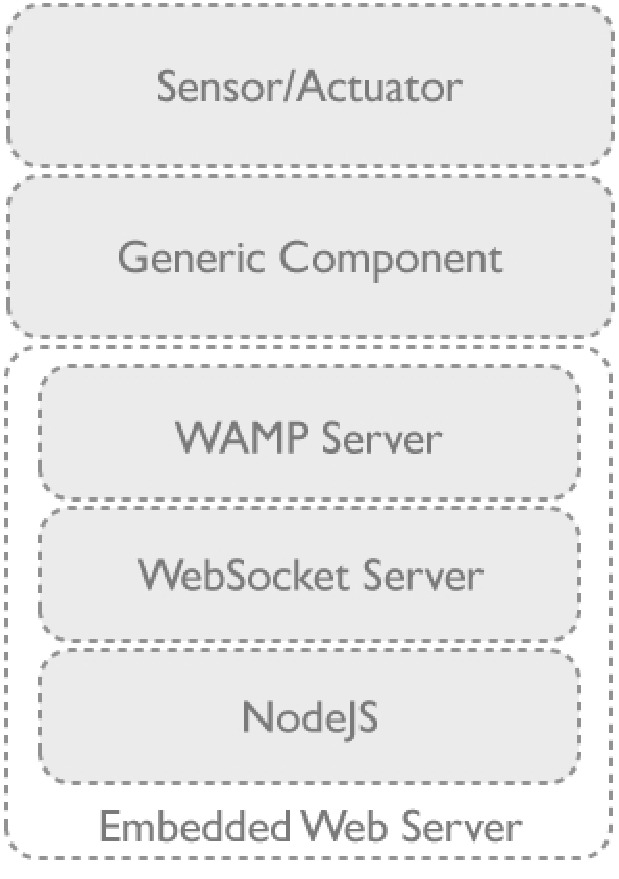
\includegraphics[width=0.5\textwidth]{images/component-layer-structure.pdf}
    \caption{Component Layer Structure}
    \label{fig:component-layer-structure}
  \end{center}
\end{figure}

We added a generic component layer on the embedded web server. The generic component is an abstract layer that describes information and generic configuration of a device, e.g., component type (temperature sensor, humidity sensor or light actuator etc), device ID, returnable, timeout, data sent rate and some other hardware parameters. 

The generic component also implements a function that control the component events. For example, if the sensor should send the data in some fixed interval or the data should be sent only by signalled. In the thesis, the generic component covers sensor and actuator. Thus, we added another component layer onto the generic component. All the layers interconnected will, subsequently, play the role of sensor or actuator.

We start with the sensor. As a sensor is built on top of a generic component which handles parameters configuration and event abstraction, a sensor is capable of responding to configuration and events. As for a light sensor, the events are the followings:

\begin{itemize}
% You can use this command to set the items in the list closer to each other
% (ITEM SEParation, the vertical space between the list items) 
\setlength{\itemsep}{0pt}
\item Get current sensor data. This function triggers a sensor to retrieve data from its environment. In the sample, the sensor senses light brightness data.
\item Configuration. To configure a sensor with parameter. Sensor's action, however, is usually hardcoded and cannot be configured remotely. This is due to a security reason, that the currently implementation does not allow an action parameter (such as a function) transmitted remotely.
\item Reset. To reset the configuration of a sensor to default.
\end{itemize}

As for actuator, it is built at the same layer as that for sensor, and thus, it also inheres features from generic sensors as the sensor does. In the sample, we configure an actuator into a light switch, and it can be described as the followings:

\begin{itemize}
% You can use this command to set the items in the list closer to each other
% (ITEM SEParation, the vertical space between the list items) 
\setlength{\itemsep}{0pt}
\item Switch on. To switch on a light and regardless the light current state.
\item Switch off. To switch off a light and regardless the light current state.
\item Switch a light. To switch the light to its opposite state. This means, if a light is on, it, then, will be switched off and vice versa.
\item Adjust luminance. To adjust a light luminance to a given value which should be in the range of a light acceptable value.
\item Configuration. Similar to that of a sensor.
\item Reset. Similar to that of a sensor.
\end{itemize}

In effect with simulation, we added an virtual component that simulates a light. Thus, a light status (on or off) can be check through this component. 

Summary so far, the interface of a light sensor/switch (sensor/actuator) can be illustrated in Figure \ref{fig:component-interface}. in a generic way:

\begin{figure}[ht]
  \begin{center}
    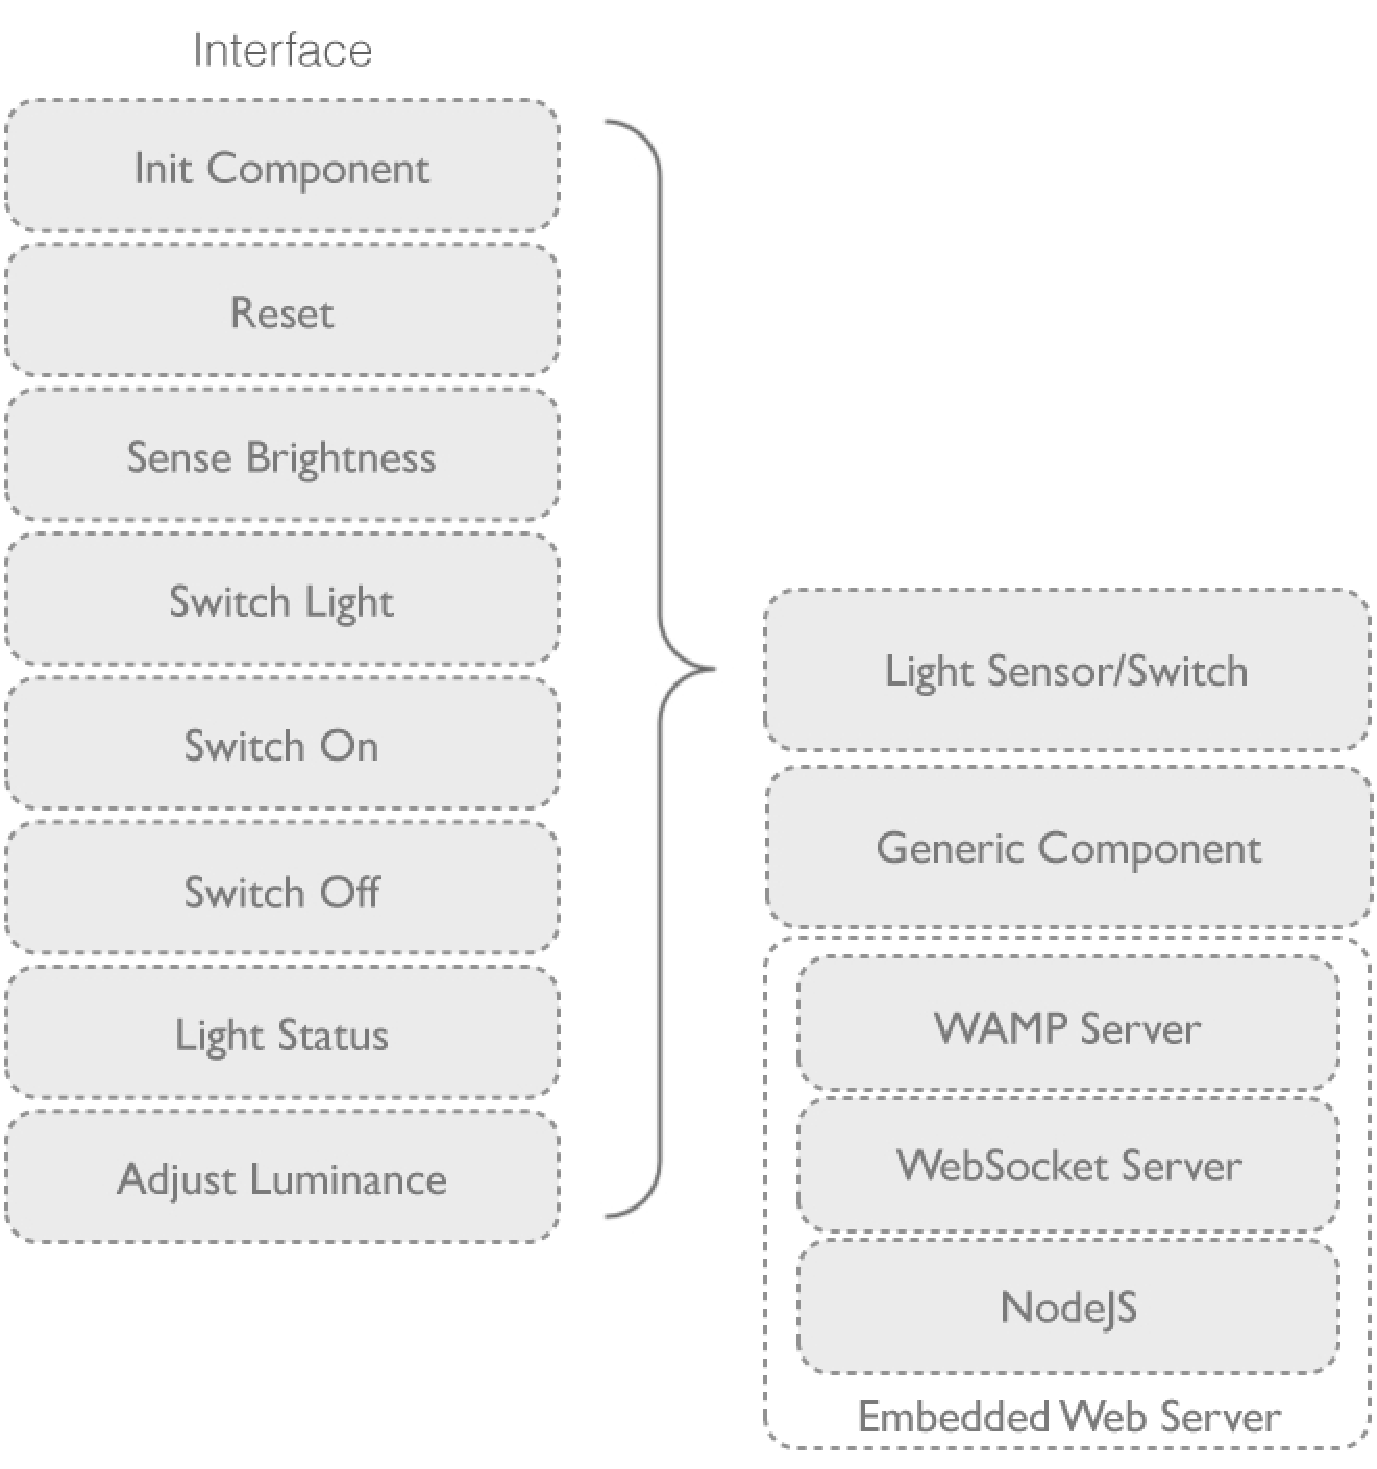
\includegraphics[width=0.7\textwidth]{images/component-interface.pdf}
    \caption{Component Interface}
    \label{fig:component-interface}
  \end{center}
\end{figure}

To view the architecture, at a higher level, which we have exposed so far, the light sensor and the light switch are connected to a component with an embedded web server, or separately. This architecture is shown in Figure \ref{fig:component-nodeJS-interface}.

\begin{figure}[ht]
  \begin{center}
    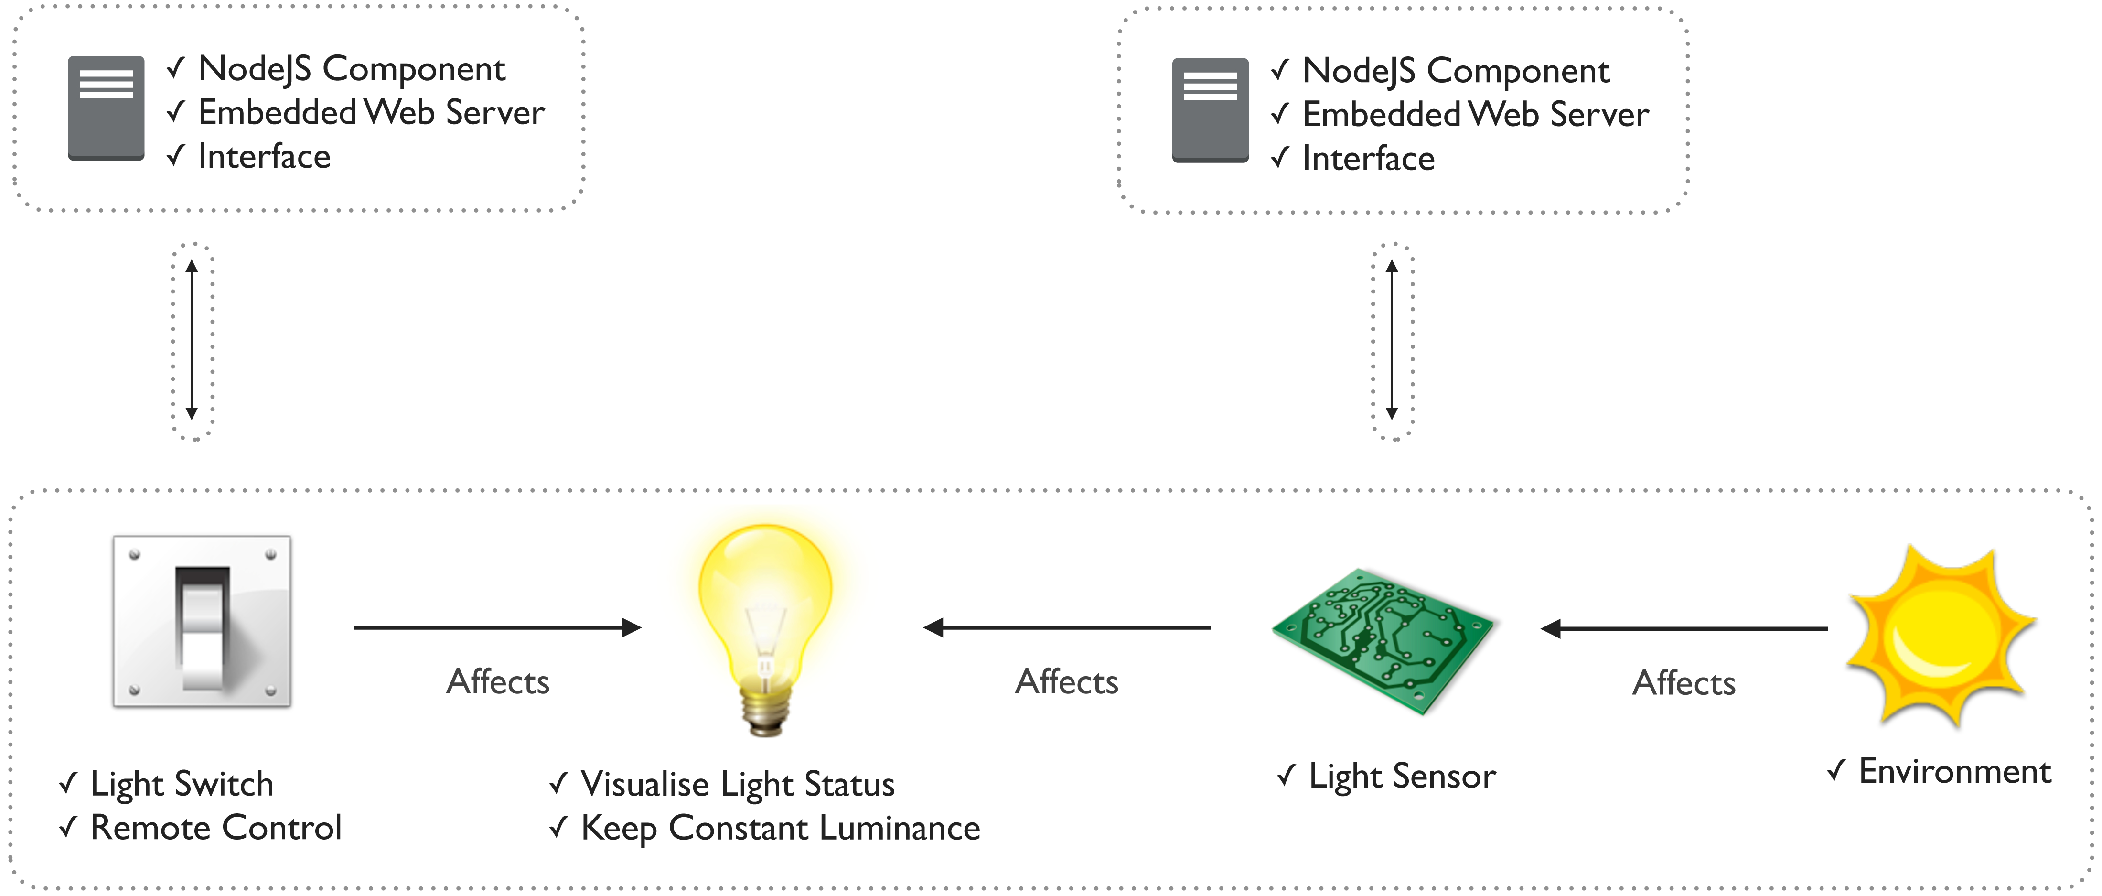
\includegraphics[width=1\textwidth]{images/component-nodeJS-interface.pdf}
    \caption{Components Connected to Embedded Web Server}
    \label{fig:component-nodeJS-interface}
  \end{center}
\end{figure}

The light sensor and the light switch are linked to a component respectively. The two components differ themselves by the topmost layer which we showed in Figure \ref{fig:component-layer-structure}. With the embedded web server, the light sensor and the light switch can communicate with each other and other components (such as the simulated component, light) over WebSockets. We can think this way, the component, which the light switch connected to, enhance the functionality that the light switch can do. For example, it controls the light via the interface switch on/off. 

\subsection{Implementation of The Front-end}
However, the current system should be accessible from outside, such as by end users. We implemented this via a web front-end interface. 

The structure is layered at front. Concerning the connection is over WebSocket, a WebSocket layer is arranged at the bottom. The WebSocket layer handles the connection with the embedded web server. 

The communication coming from the embedded web server, is however, using WAMP protocol. Thus, we added another layer, WAMP layer, on top of the WebSocket layer. With these two layers, the front-end and the backend can, now, communicate.

We also would like to control the backend, and thus we added another layer, APIs layer, on top of the WAMP layer. The APIs layer contains light sensor APIs and light switch APIs. As the name implies, programmers can control the backend through the APIs that this layer provides. For example, with the APIs, we can make a web interface that visualises the light switch which can response to users click event and subsequently control the light on and off; we can also visualise the light status on a web interface, so we can check the light status remotely. 

This architecture is shown in Figure \ref{fig:front-end-layer-structure}.

\begin{figure}[ht]
  \begin{center}
    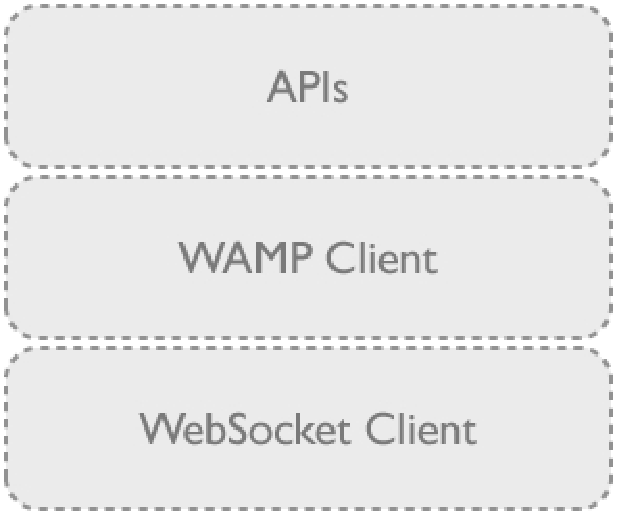
\includegraphics[width=0.5\textwidth]{images/front-end-layer-structure.pdf}
    \caption{Front-end Layer Structure}
    \label{fig:front-end-layer-structure}
  \end{center}
\end{figure}

\subsection{Overall Structure}
We have covered end users, front-end structure and backend structure. Now, we can link them together. This architecture is shown in Figure \ref{fig:communication-structure-with-user}.

\begin{figure}[ht]
  \begin{center}
    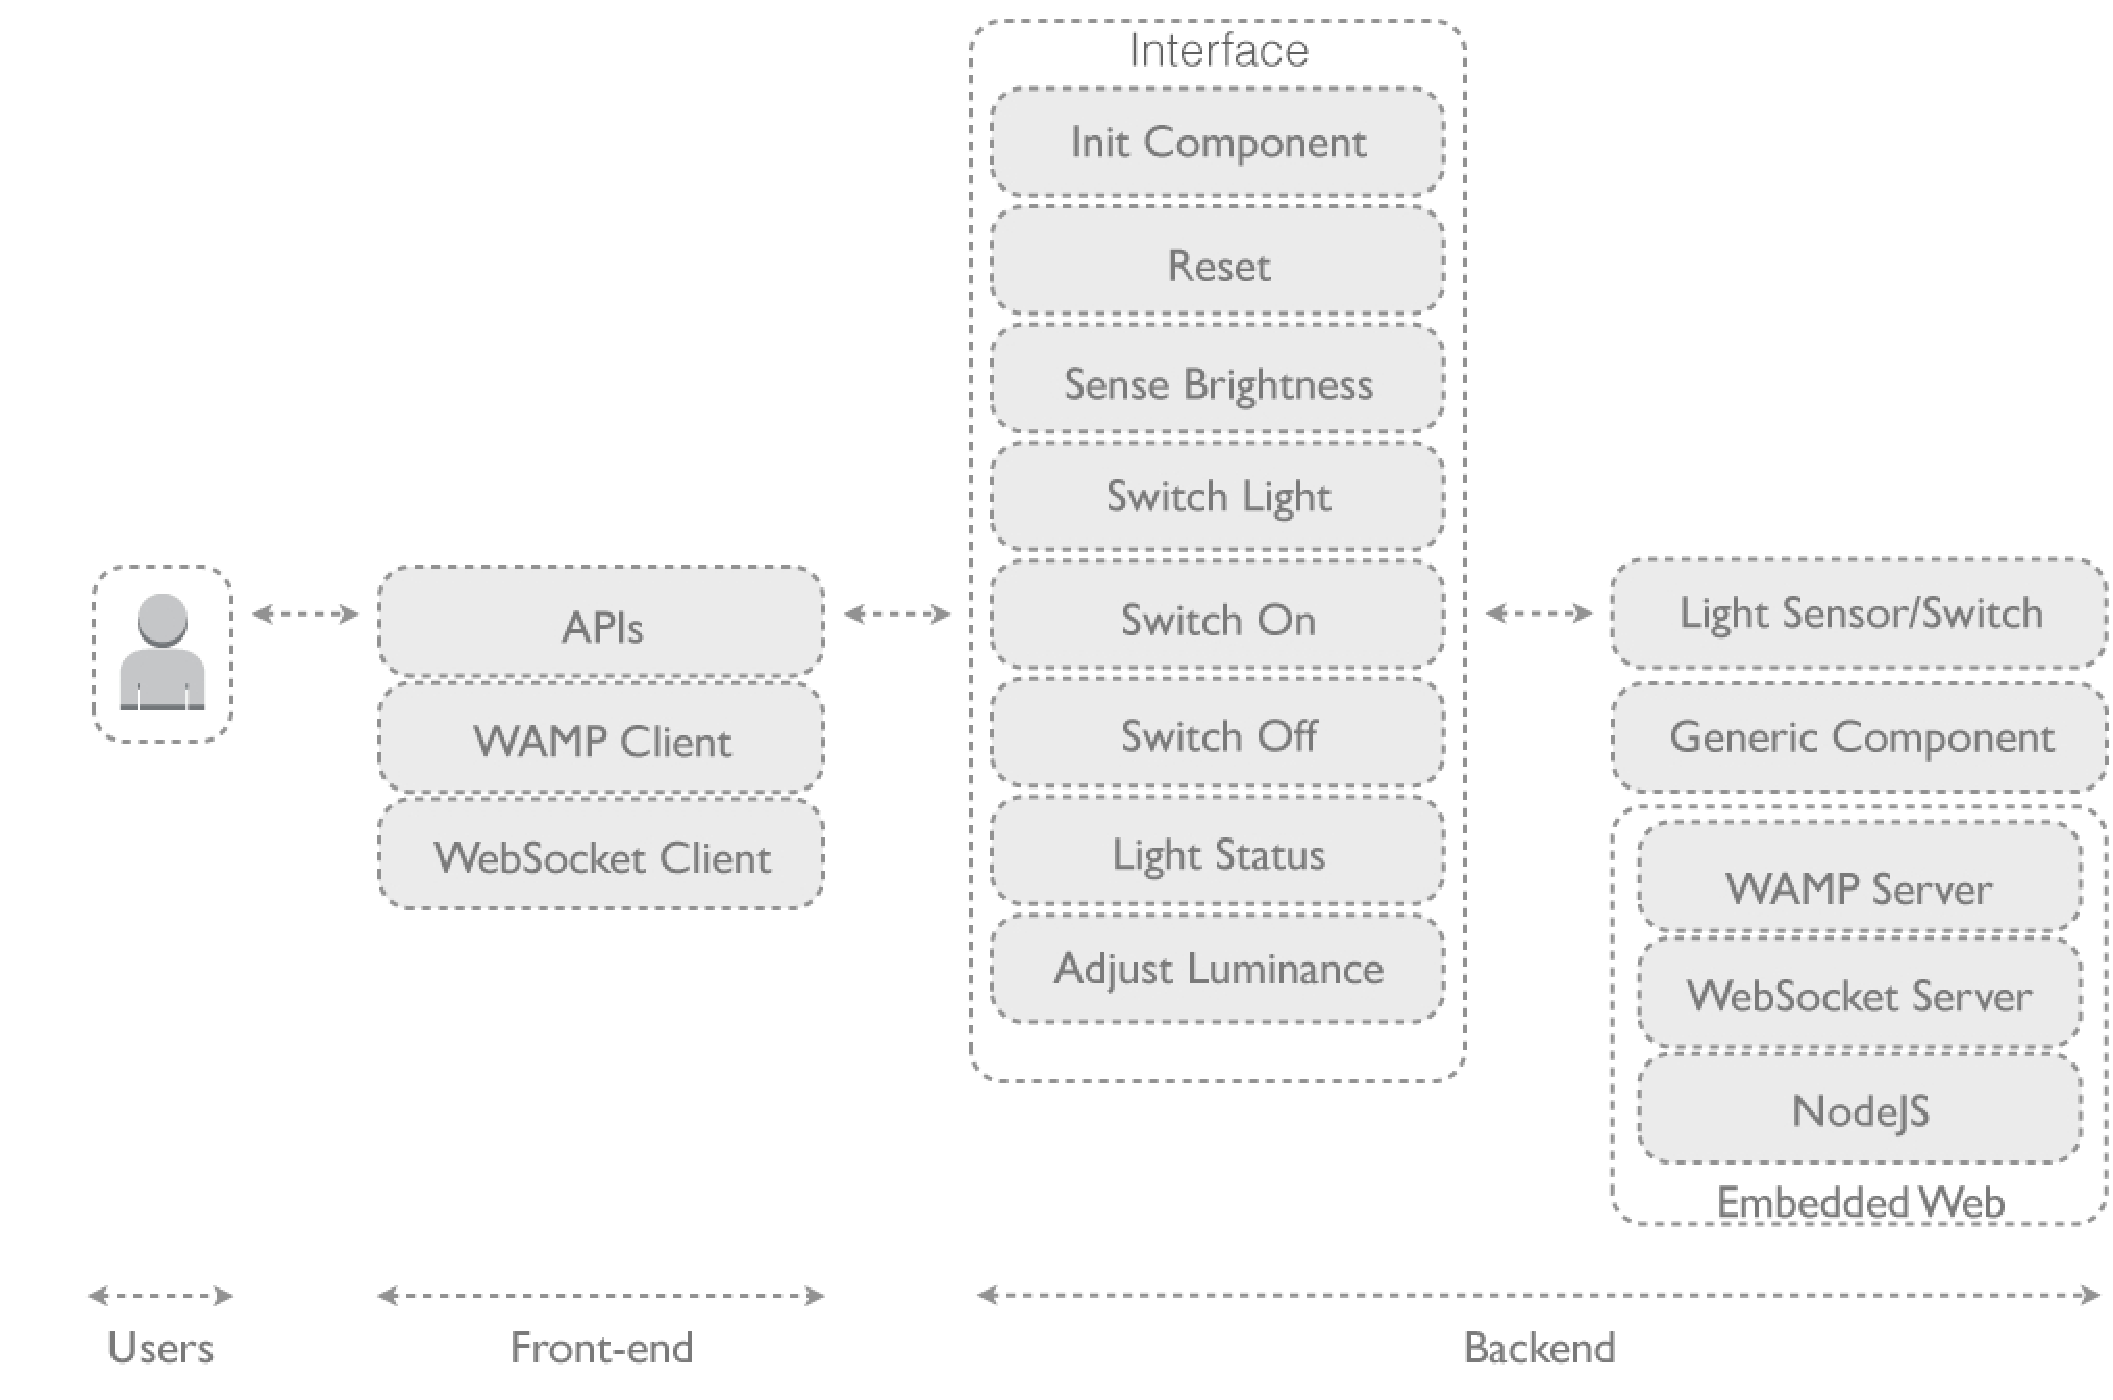
\includegraphics[width=1\textwidth]{images/communication-structure-with-user.pdf}
    \caption{Overall Structure}
    \label{fig:communication-structure-with-user}
  \end{center}
\end{figure}

The APIs layer connects users and the interface provided by the backend. WAMP Client talks with WAMP server through WebSocket Client which talks with WebSocket Server.

\subsection{The Role of Messaging Patterns}
Previously, we have discussed Pub/Sub and RFC. These two pattens, handled by WAMP layer, cover the two most important interactions in Internet of Things: notification and command. Here, we discuss how are they integrated in the sample. This architecture with message patterns is shown in Figure \ref{fig:message-pattern-overall-structure}.

\begin{figure}[ht]
  \begin{center}
    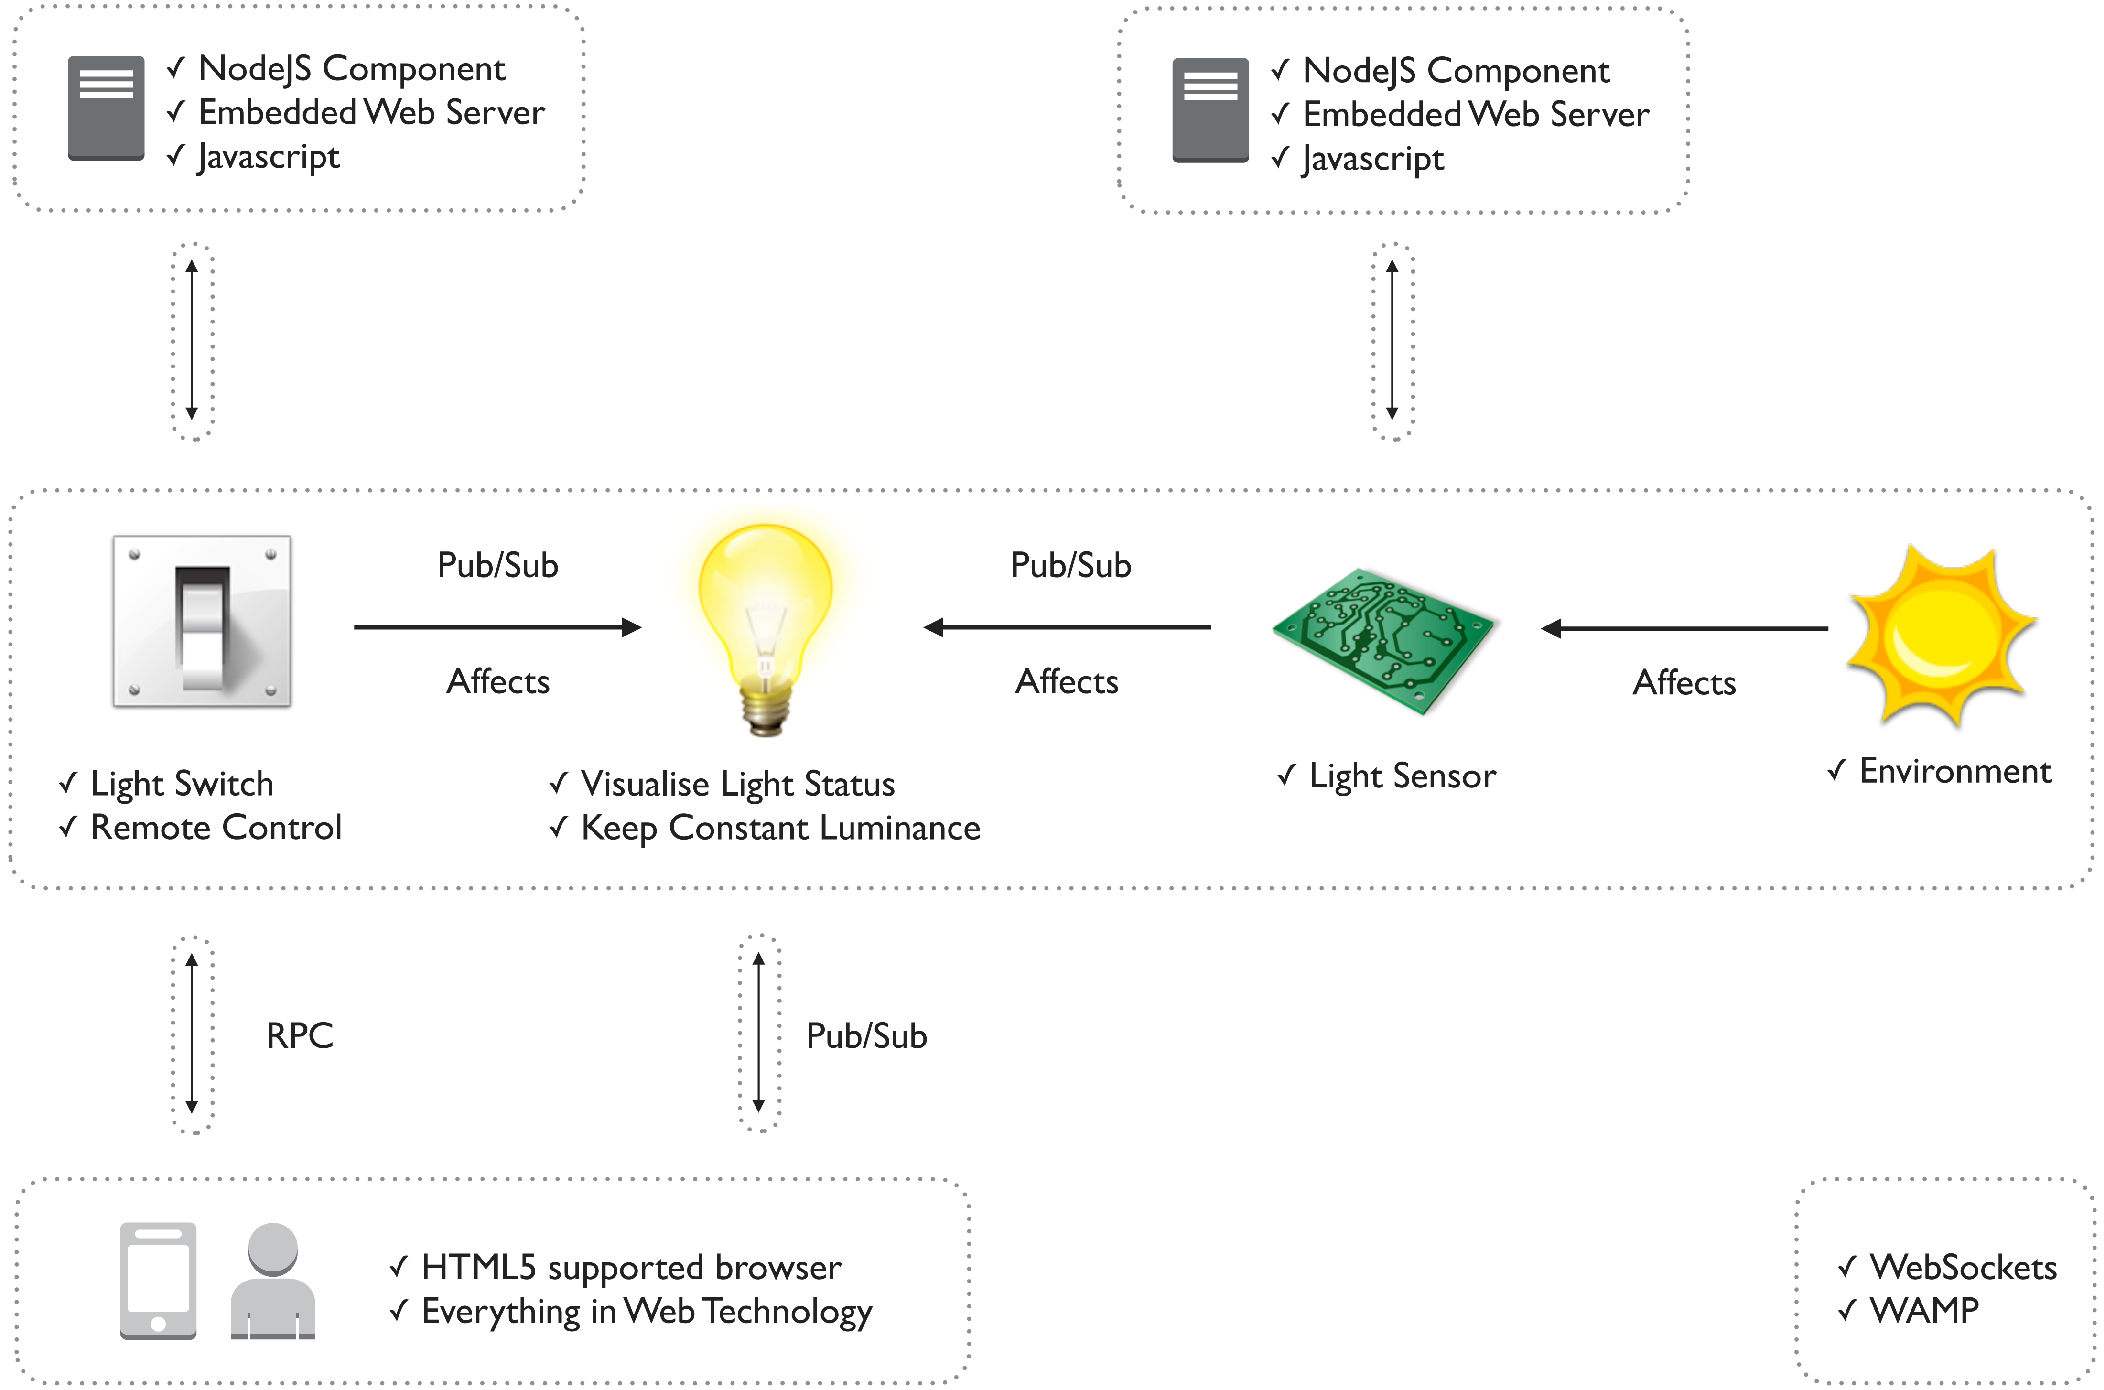
\includegraphics[width=1\textwidth]{images/message-pattern-overall-structure.pdf}
    \caption{Overall Structure with Massage Patterns}
    \label{fig:message-pattern-overall-structure}
  \end{center}
\end{figure}

As the front-end is built with HTML5 technology, the sample is capable with any browser that supports HTML 5 feature (WebSocket). Thus, the architecture is designed in a way that end users can control the light switch and view the light status via a browser. 

When a end user control the light switch, such as turning on the light; turning off the light; or adjusting the luminance of the light, it sends the command using RPC patterns. RPC pattern is also applied in component initialisation and reset. When the user view the visualisation of the light status, it communicates with the components via Pub/Sub patterns.

The interaction between the light switch and the light is using Pub/Sub pattern. The light component subscribes a topic from the light switch. When the user e.g. turns on the light, the switch component publishes a message with the light on value (such as, true) to the light component. The light component, then, receives the message, processes the message and turn on the light. Luminance adjustment is similar.

The interaction between the light sensor and the light is, also, Pub/Sub pattern. The light component subscribes a topic from the light sensor, as opposed to that from the light switch. When the light sensor updates its collected data, the light receives the data and subsequently adjust the light luminance according to its setting.

\section{Social Sensing}
In contrast to the WebSocket based sample: Smart Lighting and Control Application, we provided another sample IoT service, Social Network IoT Sensing Application, based on data centralised model using HTTP for communication. 

\subsection{Features}
The sample application provides a way to visualise data collected by IoT devices remotely in nearly real-time. For example, a user deploys IoT devices at home. The devices, then, collect temperature, humidity and multimedia (image, video, and audio) data at home. The purpose of the design enables the user to inspect those data in a visualised way from a browser. Visualisation means, for example, a graph chart of the temperature of the user's home within the past 24 hours. Real time means, for example, the web interface updates corresponding to live notification, once the collected data have been processed.

Furthermore, the sample application is extensible by integrating third party APIs. For example, the sample could visualised IoT devices geo-locations and geographic structures, with Google Map APIs; Notification could be extended into the area of social network, other than the owner exclusively. 

The underlying infrastructure of application handles scaling such as distributing and clustering. This feature satisfies the same demand in IoT services.

\subsection{Stack and Architecture}
Social Network IoT Sensing Application is a CouchApp\footnote{http://couchapp.org/page/index}, a Javascript and HTML5 application served directly from CouchDB. CouchDB is a documented-oriented database. Data are stored in JSON documents and are accessed with a web browser via HTTP. CouchDB is, also, designed for data distribution and replication. In short, CouchDB provides scalability and flexibility. These features are meaningful to the challenges\cite{francesco2012storage} - heterogeneity and scale - in IoT services. Its layer stack is shown in Figure \ref{fig:data-centre-app-stack}.

\begin{figure}[ht]
  \begin{center}
    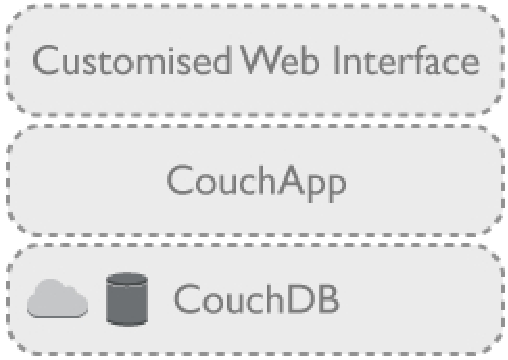
\includegraphics[width=0.5\textwidth]{images/data-centre-app-stack.pdf}
    \caption{Social Network IoT Sensing Application Layer Stack}
    \label{fig:data-centre-app-stack}
  \end{center}
\end{figure}

CouchDB acts as an HTTP server, serving HTML directly to a browser, while manages heterogeneous data and horizontal scaling; CouchDB, moreover, provides live notifications and handles over the notifications to upper layers. External data, such as collected by IoT devices, connect to CouchDB via a gateway. The collection of the data and the purpose of the gateway have been discussed in \cite{francesco2012storage}. 

CouchApp inherited these features from CouchDB. Furthermore, CouchApp is extensible. Thus, we have a third layer to extend the functionality and customise the usability. For instance, we used BackboneJS, Model-View (MV) Javascript library, to structure our application. Third party APIs, additionally, can be integrated into the third layer and thus enable, e.g. social network or geography functions. End users interact with the system via the third layer. 

The architecture of the sample application is shown in Figure \ref{fig:data-centre-architecture}.

\begin{figure}[ht]
  \begin{center}
    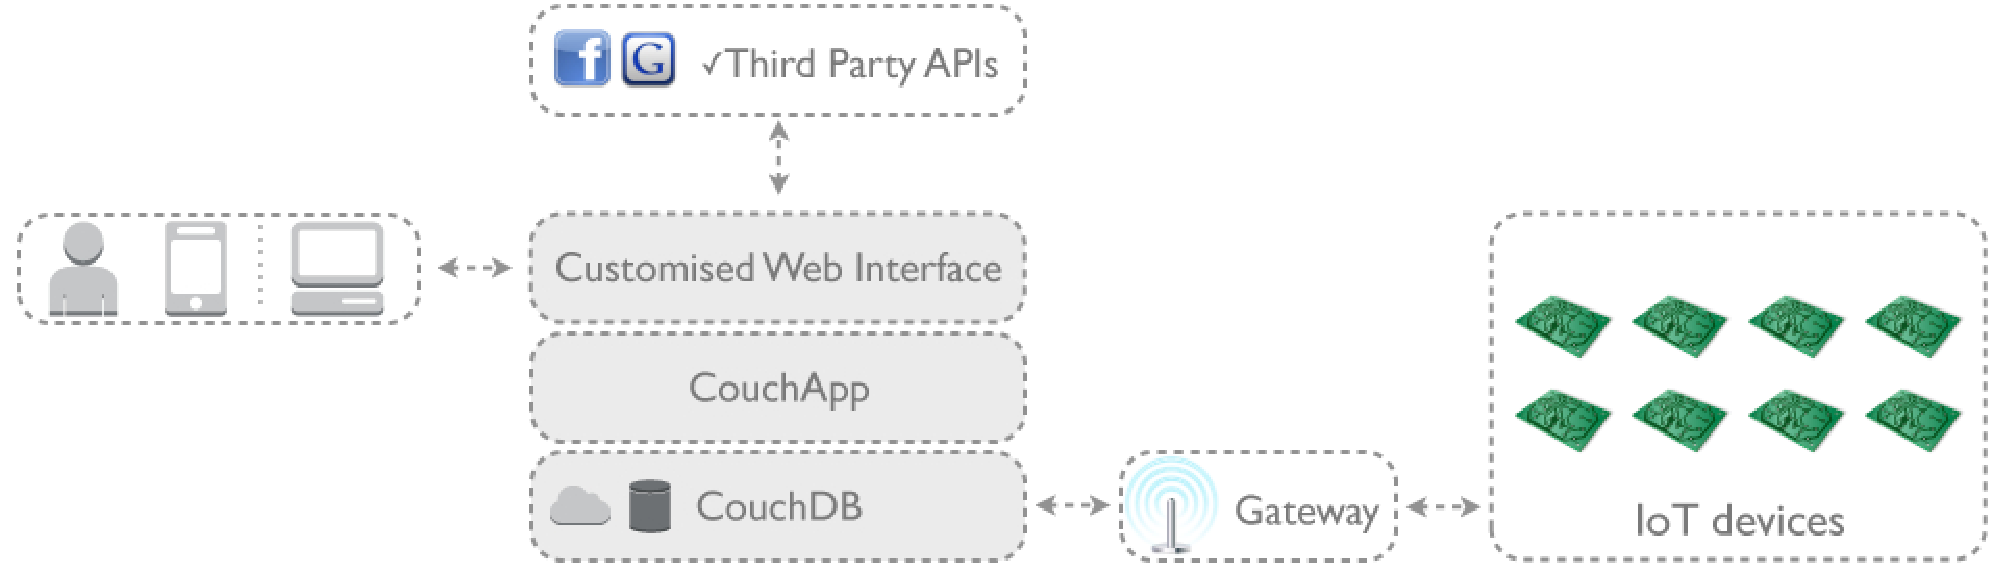
\includegraphics[width=1\textwidth]{images/data-centre-architecture.pdf}
    \caption{Social Network IoT Sensing Application Architecture}
    \label{fig:data-centre-architecture}
  \end{center}
\end{figure}

\subsection{Retrieving Data}
The architecture, which end users directly interacting with, is based on a HTTP web server, CouchDB. Thus, all connections are HTTP based. In order to keep notification alive, the browser has to maintain HTTP connections, negotiate with the web server, update HTTP connections and keep HTTP connection alive. 


 

%!TEX root = /Users/Ken/Dropbox/Master's Thesis/Paper/my thesis/main.tex
\chapter{Evaluation}
\label{chapter:evaluation}

\section{Reference Scenario}
We planned to build an IoT service with web technology that differed from the pervious solution, database-centric approach, which largely relies on Ajax for data exchange. 

The prevision of the thesis was constructed in two parts: web technology and IoT; Its solution should integrate the two parts into a coherent service. Following the consideration of HTML5 connectivity features, we focused on the WebSocket protocol which fills the part of web technology. As for IoT, which covers a wide area, we selected one scenario -- smart lighting control -- with a sensor and an actuator from many IoT visions such as NFC applications, smart housing and phones connectivity. 

Compared with other HTML5 communication technologies, the WebSocket protocol is more mature, having ready made auxiliary libraries with a feasible amount of selections. The WebSocket protocol, additionally, supports subprotocols where WAMP fills the blank and provides the messaging patterns which furthermore covers the two most important interaction in IoT service.

The Sensor and actuator are two of the most common ``things'' in IoT architecture. The sensor collects data, while the actuator emits commands. We evaluated these two components matches the web technology, WebSockets with WAMP. We, further, collected several IoT scenario assumptions - high lever descriptions of what we thought might work. For example, we drafted using sensors in a phone, collected data and reported to data centre; Applying a searching function in the real world; or smart building. We evaluated the phone case is a bit far away from web technology and the implementation might involve more mobile technology rather than web technology. As for the searching function, it might involve more hardware configurations and physical experiments. 

Among of all, thus, we trimmed down the assumptions and focused on the smart building scenario. We proposed several hypotheses -- more granular descriptions of the assumption -- which target on the following specific areas: sensor deployment, data collection, data transmission, endpoint visualisation and others, such as business model level cases. Moreover, we continuously decreased the amount of areas to work on. Data transmission is related to the thesis scope where it matches Pub/Sub and RPC patterns; While endpoints visualisation provides a human friendly interface to review data, and it, besides, performs simulation, such as, simulating the environment.

Finally, we started to experiment on the smart lighting and control application, an IoT service about a sensor and an actuator with the WebSocket. 

\section{Tools and Setup}
Before we started the thesis project, we assumed the front-end environment would largely rely on web browsers. As a result, we expected to build it with JavaScript. For this reason, we found AutobahnJS\footnote{http://autobahn.ws/js}, an open source JavaScript networking library. 

AutobahnJS supports WAMP at a higher level, while supports the WebSocket protocol at lower level. Thus, it is feasible to create a real-time enabled HTML5 applications with the library. Moreover, AutobahnJS has - another advantage of AutobahnJS - clear tutorials and documents.

As for the backend deployment, it relatively has more options where a list of existing library has been being appended to support WAMP. From the perspective of programming languages, there are implementation on Python, PHP, JavaScript, Java and others. Our implementation is based on WAMP.IO, a NodeJS library supporting WAMP. WAMP.IO does not handle the WebSocket protocol, but its dependency does. 

At the beginning, there were some technical problems in WAMP.IO, leading an initial connection failure with a WAMP client. Thus, we moved to Ratchet, a backend implementation using PHP, until the developer fixed those problems. Compared WAMP.IO with Ratchet, we found out Ratchet is more verbose, from the perspective of development: there are some features we did not need. WAMP.IO, however, targets the desired features - Pub/Sub and RPC - straightforward. With its simple architecture, we could easily customise the library to match demands more closely. Moreover, its developer, behind the library, actively identified and fixed bugs, making the whole development reliable. 

\section{Simulation}
We mentioned about the light, the switch/dimmer, the sensor and the sun in the thesis. Considering the thesis scope, we decided to focus on the software level, rather than the hardware part. Thus, we, at the current stage, simulated the light, the switch, the sensor and the sun. 

For the simulation, we ported the most relevant features - directly related to the implementation - to the software level. Meanwhile, we analysed its possibility bringing those features and the results back to physical objects. 

For example, a light bulb emits light, where the light is the key link connecting the virtuality to the reality. We mapped light luminance into digital numbers at the software level. The luminance can thus be controlled by adjusting digital numbers. The light status - on and off - similarly, can be simulated by e.g. boolean value. 

As for the switch/dimmer, a switch turns on or off the light, while a dimmer adjusts the luminance of the light at a certain range. The action of turning/adjusting is the key part that we simulated. The simulation of turning/adjusting, is, being the case, to connect the light component and the switch/dimmer component at the software level, and making the light response to the action of the switch/dimmer. This is, actually, how a switch/dimmer does in the real world.

A sensor, generally, converts physical quantity into digital signal which can be further read or analysed by a observer or an instrument. Thus, a sensor is, essentially, a programme that provides data at the software level. Consequently, we simulated the sensor through a programme piping the output of the sun to the light.

As for the sun, we also ported it to the software level. To do so, we made a programme that generated a sequence of numbers periodically increasing to a peak then recurring.

\section{Measurements}
We measured about overheads and Roundtrip Delayed Time (RTT) comparing WAMP with MQTT. Figure \ref{fig:overhead} illustrates the message overheads on WAMP and MQTT.

\begin{figure}[t]
  \begin{center}
    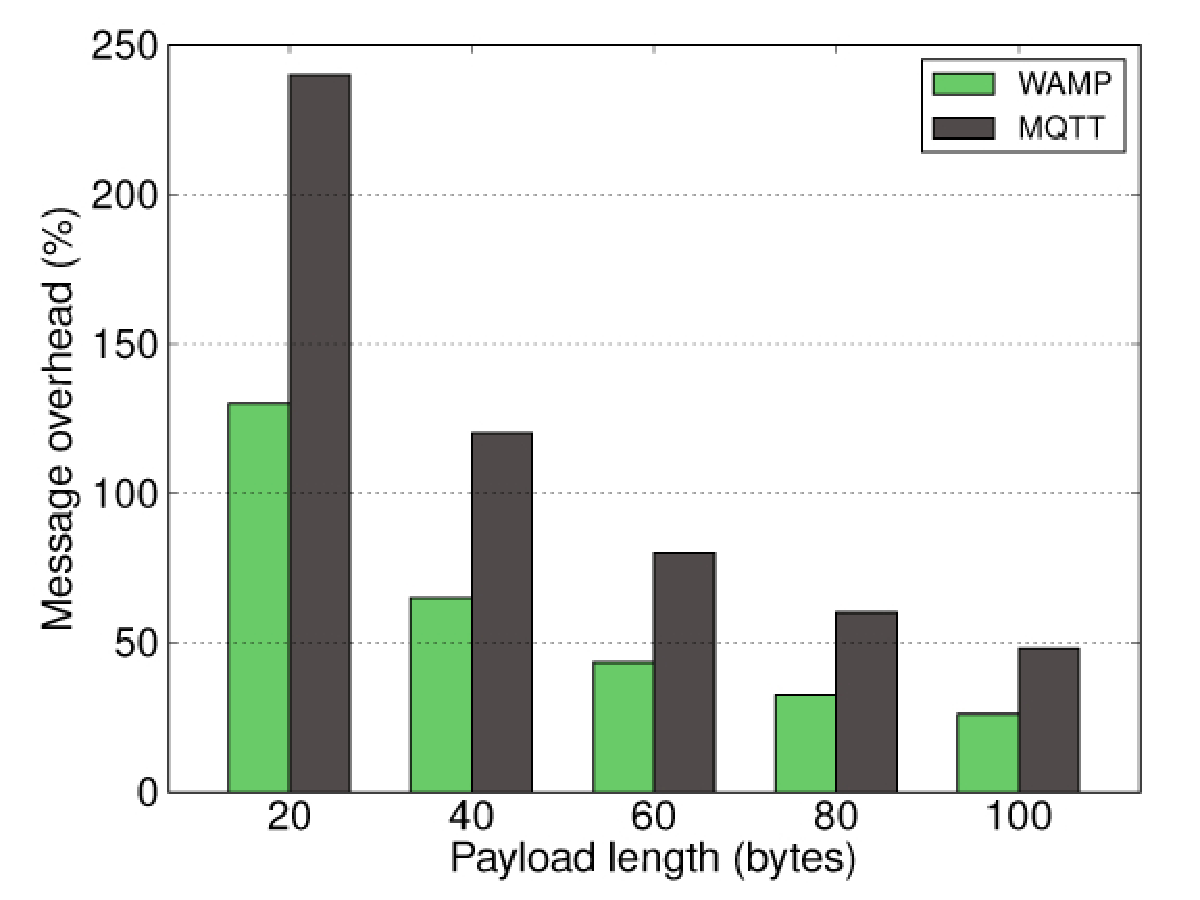
\includegraphics[width=0.7\textwidth]{images/overhead.pdf}
    \caption{Message Overhead}
    \label{fig:overhead}
  \end{center}
\end{figure}

WAMP shows its lightweight design better than that of MQTT. For each 20 bytes of data sent, WAMP will have 1.25 times overheads larger than the message itself, while MQTT will have around 2.4 times overheads generated. 

Figure \ref{fig:rtt} illustrates the message RTT on WAMP and MQTT.

\begin{figure}[t]
  \begin{center}
    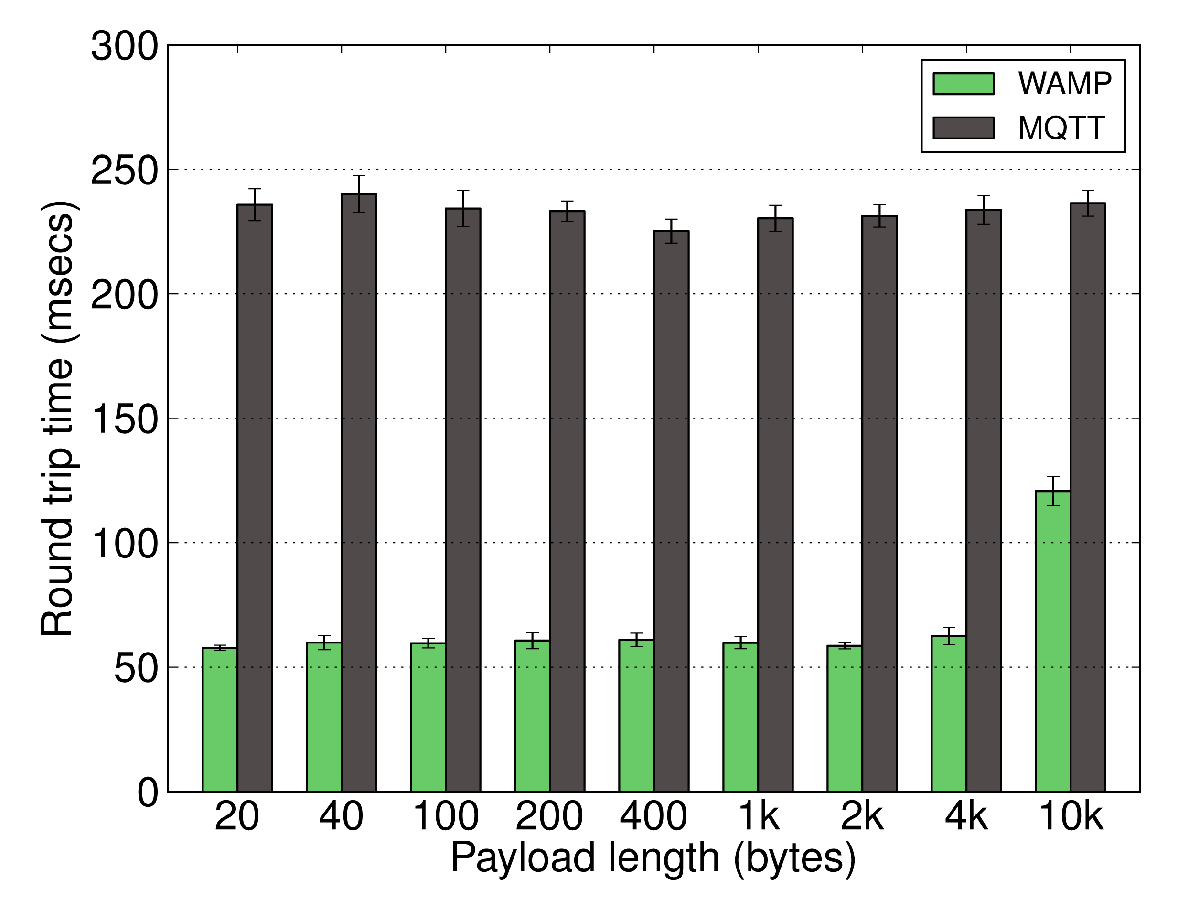
\includegraphics[width=0.7\textwidth]{images/rtt.pdf}
    \caption{Message RTT}
    \label{fig:rtt}
  \end{center}
\end{figure}

We measured the RTT from a local workstation to an Amazon micro instance in Ireland. And the result we got is, generally, MQTT has a longer RTT than that of WAMP; WAMP RTT starts to increase after sending 10k bytes, while MQTT stays constantly. The sudden increment could be caused by the programme design, the workstation or the Amazon instance we used. As the package size increased, the processing and queueing time might consequently enlarge. 

\section{Scalability}
In Pub/Sub and RPC Patterns for Web-based IoT applications, the broker(s) plays a key role managing the interconnection of clients. Each client differs from others by its ID. Thus, the nature of scaling in these patterns is the implementation of addressing clients. Further communications and interactions, among users and backends, rely on the successful navigation of the broker(s).

In the scenario of the smart lighting and controlling application, the scaling issue generated by the enlarging amount of lights, switches and light sensors. Considering the limited resources that an embedded web server are assigned, the architecture might not suit for a large scale without other resources support such as extra brokers with power sources.

As for the database-centric pattern, the CouchDB solution naturally provides a reliable and flexible way to scale horizontally and to replicate, with the growing amount of data. The database acts as a hub between IoT devices and end users, while it can be further developed into cloud-based architecture which maximises its scalability. 

\section{Security}
The WebSocket protocol supports connections over Transport Layer Security (TLS). TSL provides communications security over the Internet \cite{dierks2008rfc}. Furthermore, the WebSocket protocol providers applicable security considerations as the followings \cite{rfc64552012web}: 

\begin{itemize}
% You can use this command to set the items in the list closer to each other
% (ITEM SEParation, the vertical space between the list items) 
\setlength{\itemsep}{0pt}
\item \emph{Non-browser} Client resistant. The WebSocket protocol prevents malicious running inside a web browser. 
\item \emph{Origin Considerations}. The WebSocket protocol provides a way for servers that do not intend to process input from web pages from other origins.
\item \emph{Masking}. All data from clients to servers are masked, so that the attacker does not have knowledge about how the data being sent.
\end{itemize}

The security considerations on database-centric pattern implemented by CouchDB has been discussed in \cite{francesco2012storage}. As for database, one of the most important security issue is authentication and access control. It is notable that CouchDB, by default, does not turn on access control for different users. This means, everybody has the same permission as the administrator. CouchDB authenticates users in many ways, such as HTTP basic authentication, cookie authentication and OAuth \cite{hammer2010oauth}. CouchDB has started to support Secure Sockets Layer (SSL) since CouchDB version 1.1, and thus provides communication security over the Internet.

 
\chapter{Future and Conclusion}
\label{chapter:future-and-conclusion}

At the current stage, the implementation is done at software level: hardware part are simulated. Therefore, the development process can be trimmed to fit in the scope of the thesis. However, we, carefully, preserved the essential features of each hardware component and simulated at the software level. This means, there should not be many different behaviours for further deployment on hardware components. 

One example, which could link all the features back to hardware, is Raspberry Pi\footnote{http://www.raspberrypi.org/}. Raspberry Pi supports Python as its official programming language by default, but any language which will compile for ARMv6 can be used. This implies that NodeJS can be ported on Raspberry Pi. Moreover, the embedded web sever and its upper layers, which we implemented, are not restricted by NodeJS, meaning the architecture can be built with other programming languages, such as Python. A light, a switch and a sensor can, subsequently, be connected to Raspberry Pi. We can, furthermore, use a phone's sensors as a data source, and transmit the data from the phone to Raspberry Pi.

The thesis is about applying web technology on Internet of Things. We focused on the WebSocket protocol as the part of web technology. The WebSocket creates a bi-directional connection between a server and a web browser. We highlighted its advantage by comparing it with the traditional method, HTTP, according to the behaviours of fetching resources from a web server. Furthermore, we chose WAMP as a subprotocol to support WebSocket complementarily, enabling WebSocket unprecedentedly functionality to interact with Internet of Things services. 

Moving onto the part of Internet of Things, We integrated a sensor (light sensor) and an actuator (light switch/dimmer) into the application, blending with the web technology. The major feature of the sensor (sending data) and that of the actuator (commanding and configuration) perfectly match the massage patterns, Pub/Sub and RPC, which WAMP provides. Consequently, the smart lighting and controlling Internet of Things service emerged. 

Additionally, we compared the smart lighting and controlling application with social network IoT sensing application, an application interacting with IoT services with traditional method (HTTP), from the perspective of architectures, implementation, scalability and security. 

Moreover, We compared WAMP with other registered WebSocket subprotocols: MBWS, SOAP and STOMP from the viewpoint of features; and with other potential protocols: CoAP and MQTT, from the viewpoint of practicability. We further evaluated WAMP and MQTT with communication overheads and RTT. 

There are, surely, many potential room for the future research on the blending of web technology with Internet of Things. The upsurge in bleeding-edge web technology might be supportive to the future Internet of Things services research, e.g., for the efficiency, maintainability and scalability. 


% Load the bibliographic references
% ------------------------------------------------------------------
% You can use several .bib files:
% \bibliography{thesis_sources,ietf_sources}
\bibliography{sources}

% Appendices go here
% ------------------------------------------------------------------
% If you do not have appendices, comment out the following lines
\appendix
\begin{appendices}
\chapter{Related Protocols and Formats}
\label{chapter:first-appendix}

In this appendix, we will introduce the protocols and formats that we mentioned in this thesis.

\section{JSON}

JavaScript Object Notation (JSON) is a text format for the serialisation of structured data. It is derived from the object literals of JavaScript, as defined in the ECMAScript Programming Language Standard \cite{crockford2006application}. JSON has numbers, strings, booleans and null as its primitive types. Additionally, it has objects and arrays as structured types. JSON becomes popular to exchange data between in web services or applications. With JSON, WAMP message payload is serialisable and provides data types according to those of JSON. 

\section{URI}

Uniform Resource Identifiers (URIs) provide a simple and extensible means for identifying a resource. URIs have a global scope and are interpreted consistently regardless of context \cite{masinter2005uniform}. WAMP binds to URIs by default, then it assumes global assignments and resolution to be unique. URIs are used as IDs for both topics in Pub/Sub and procedures in RPC. 

\section{XML}
Extensible Markup Language (XML) is a markup language that was designed to transport and store data. Furthermore, XML was designed to be self-describing and can be used straightforward over the Internet. XML has been widely used, for example, the SOAP protocol that we mentioned in the thesis. 


\chapter{Implementation Details}
\label{chapter:second-appendix}

In this appendix, we will show the screenshots of the aforementioned web-based applications. We will also briefly introduce the libraries we used in the implementation. 

\section{Web-based IoT Applications Screenshots}

\subsection{Smart Lighting and Control Application}

In this implementation, we used WAMP.IO\footnote{https://github.com/nicokaiser/wamp.io}, a WAMP server library, to attach to a WebSocket server running on NodeJS. As for the front-end, we used AutobahnJS\footnote{http://autobahn.ws/js}, a WAMP client library, to connect to the WAMP server.

Figure \ref{fig:screen-shot-home-auto} shows the visualisation of the lights changing according to the sun brightness, for the purpose of keeping the light brightness in a constant level.

\begin{figure}[t]
  \begin{center}
    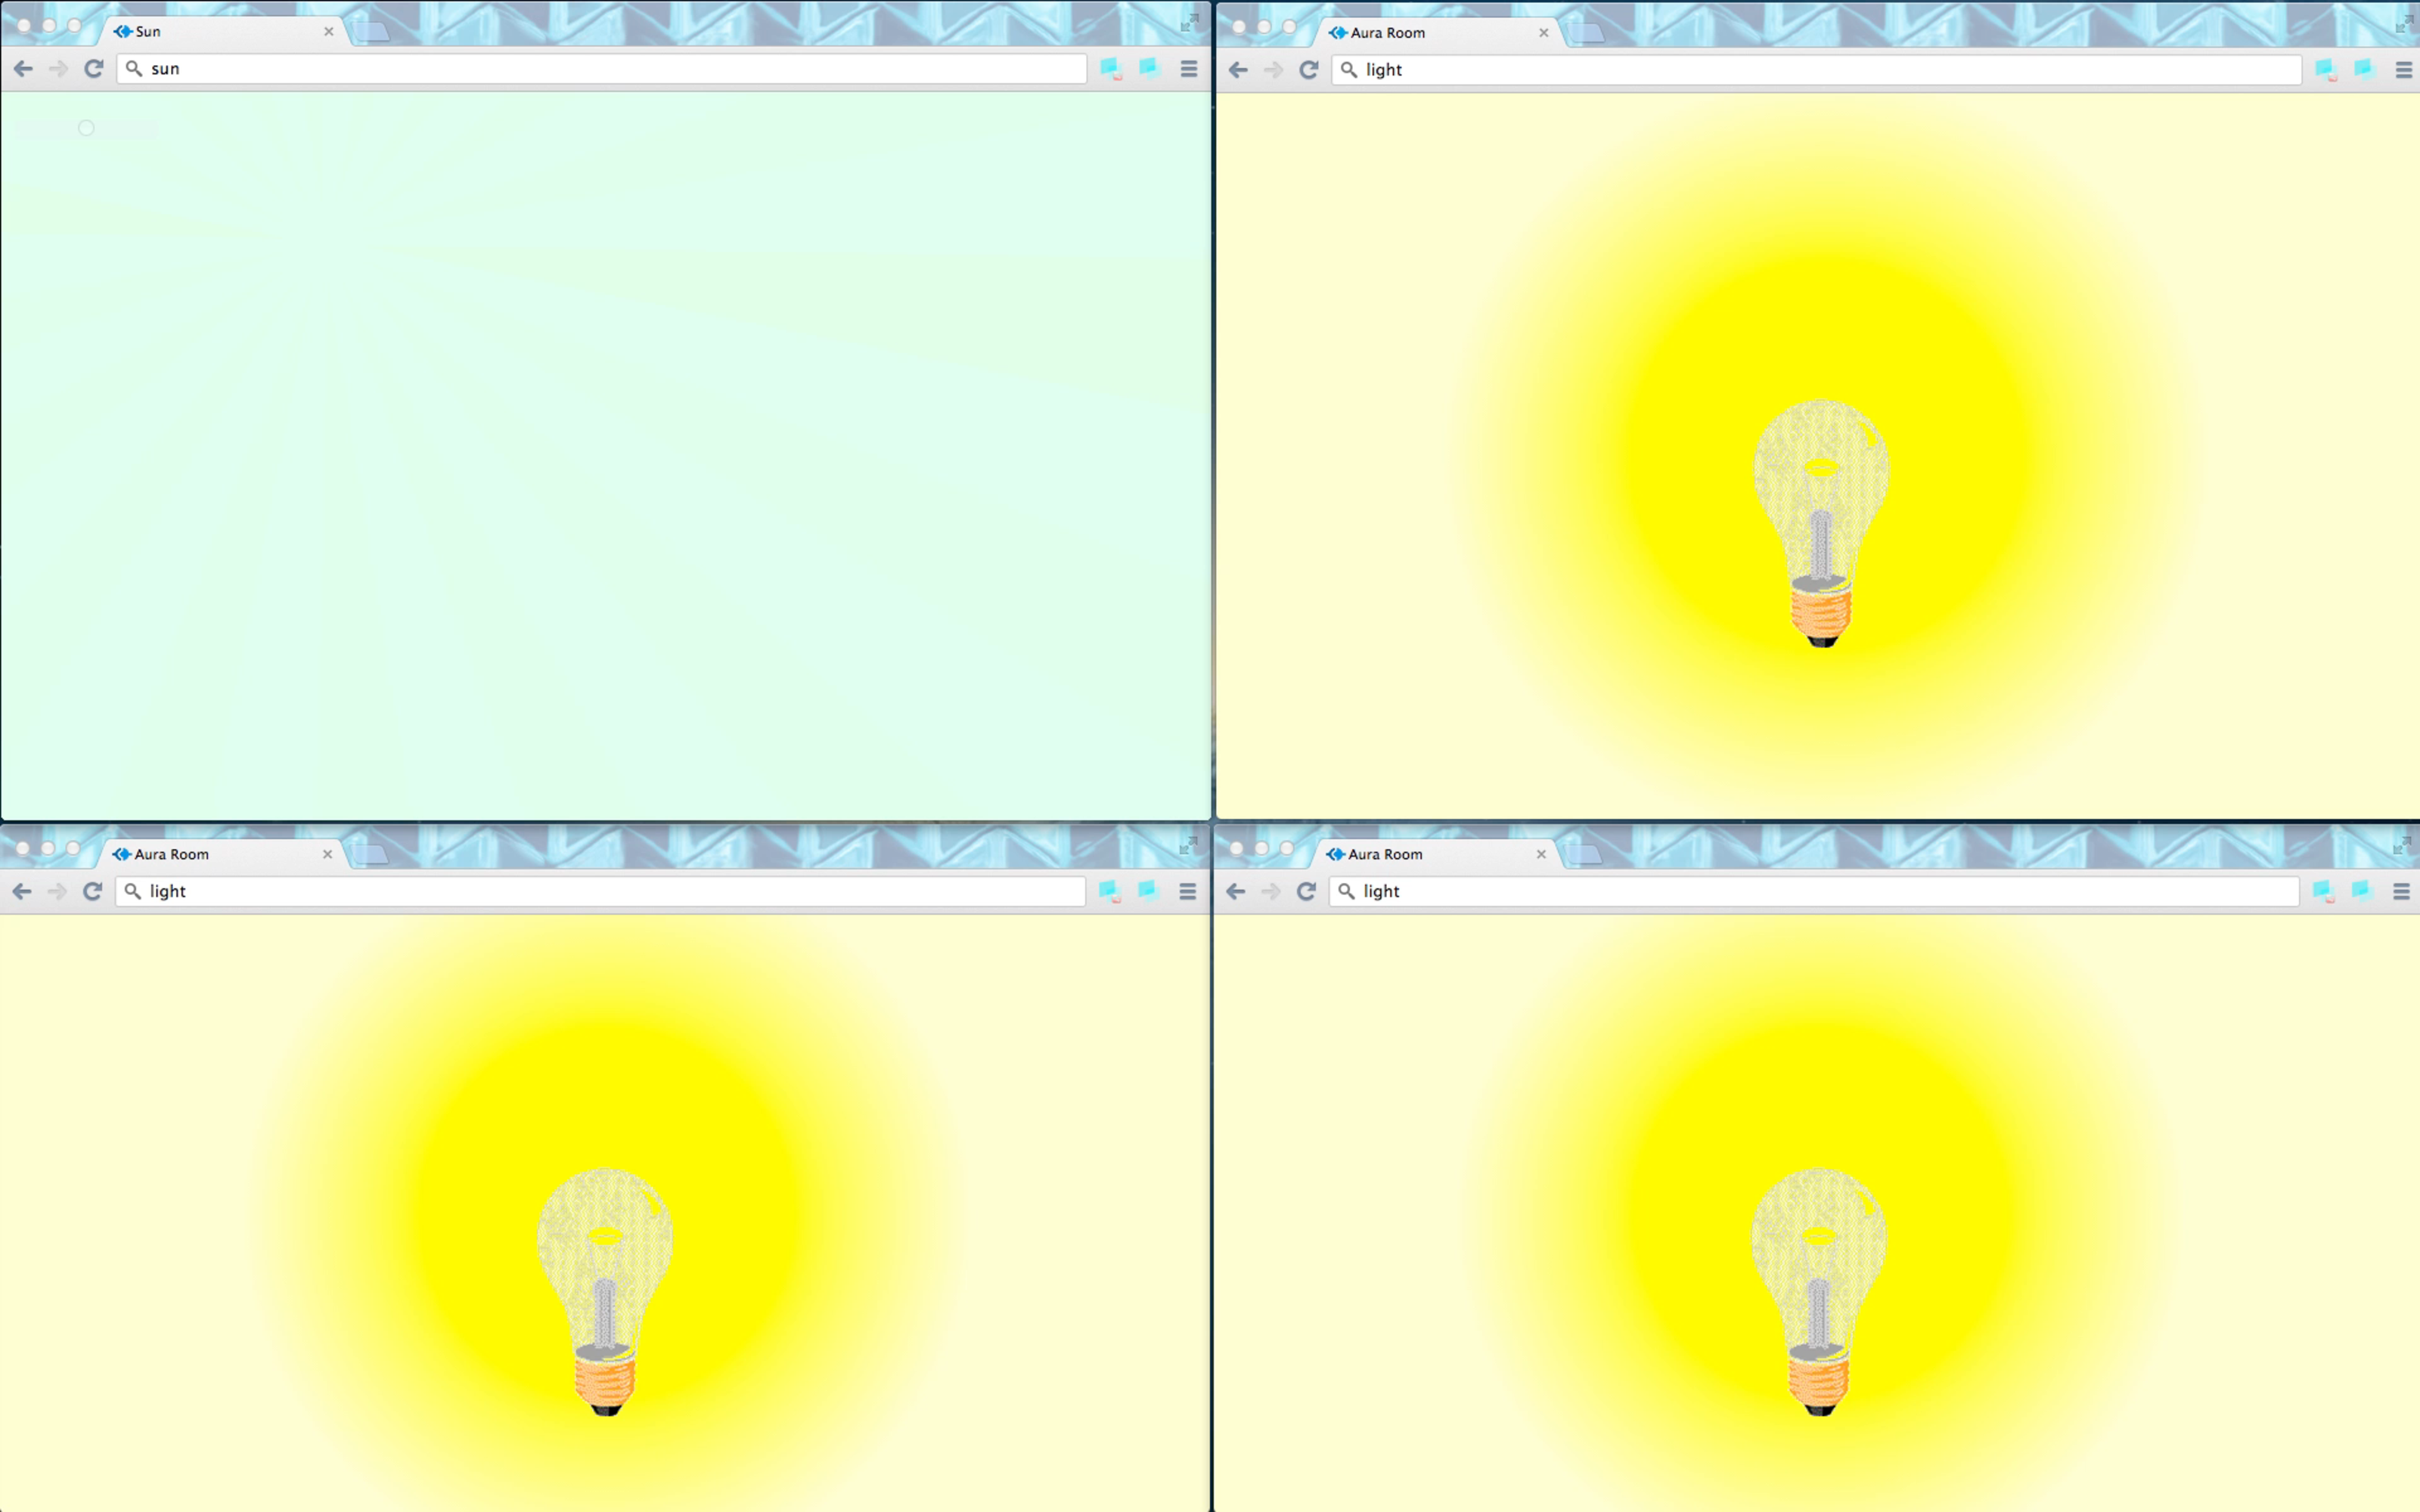
\includegraphics[width=1\textwidth]{images/screen-shot-home-auto.pdf}
    \caption{Visualisation of Lights Changing According to the Sun}
    \label{fig:screen-shot-home-auto}
  \end{center}
\end{figure}

Figure \ref{fig:screen-shot-home-auto-2} shows the visualisation of remote controlling lights status.

\begin{figure}[t]
  \begin{center}
    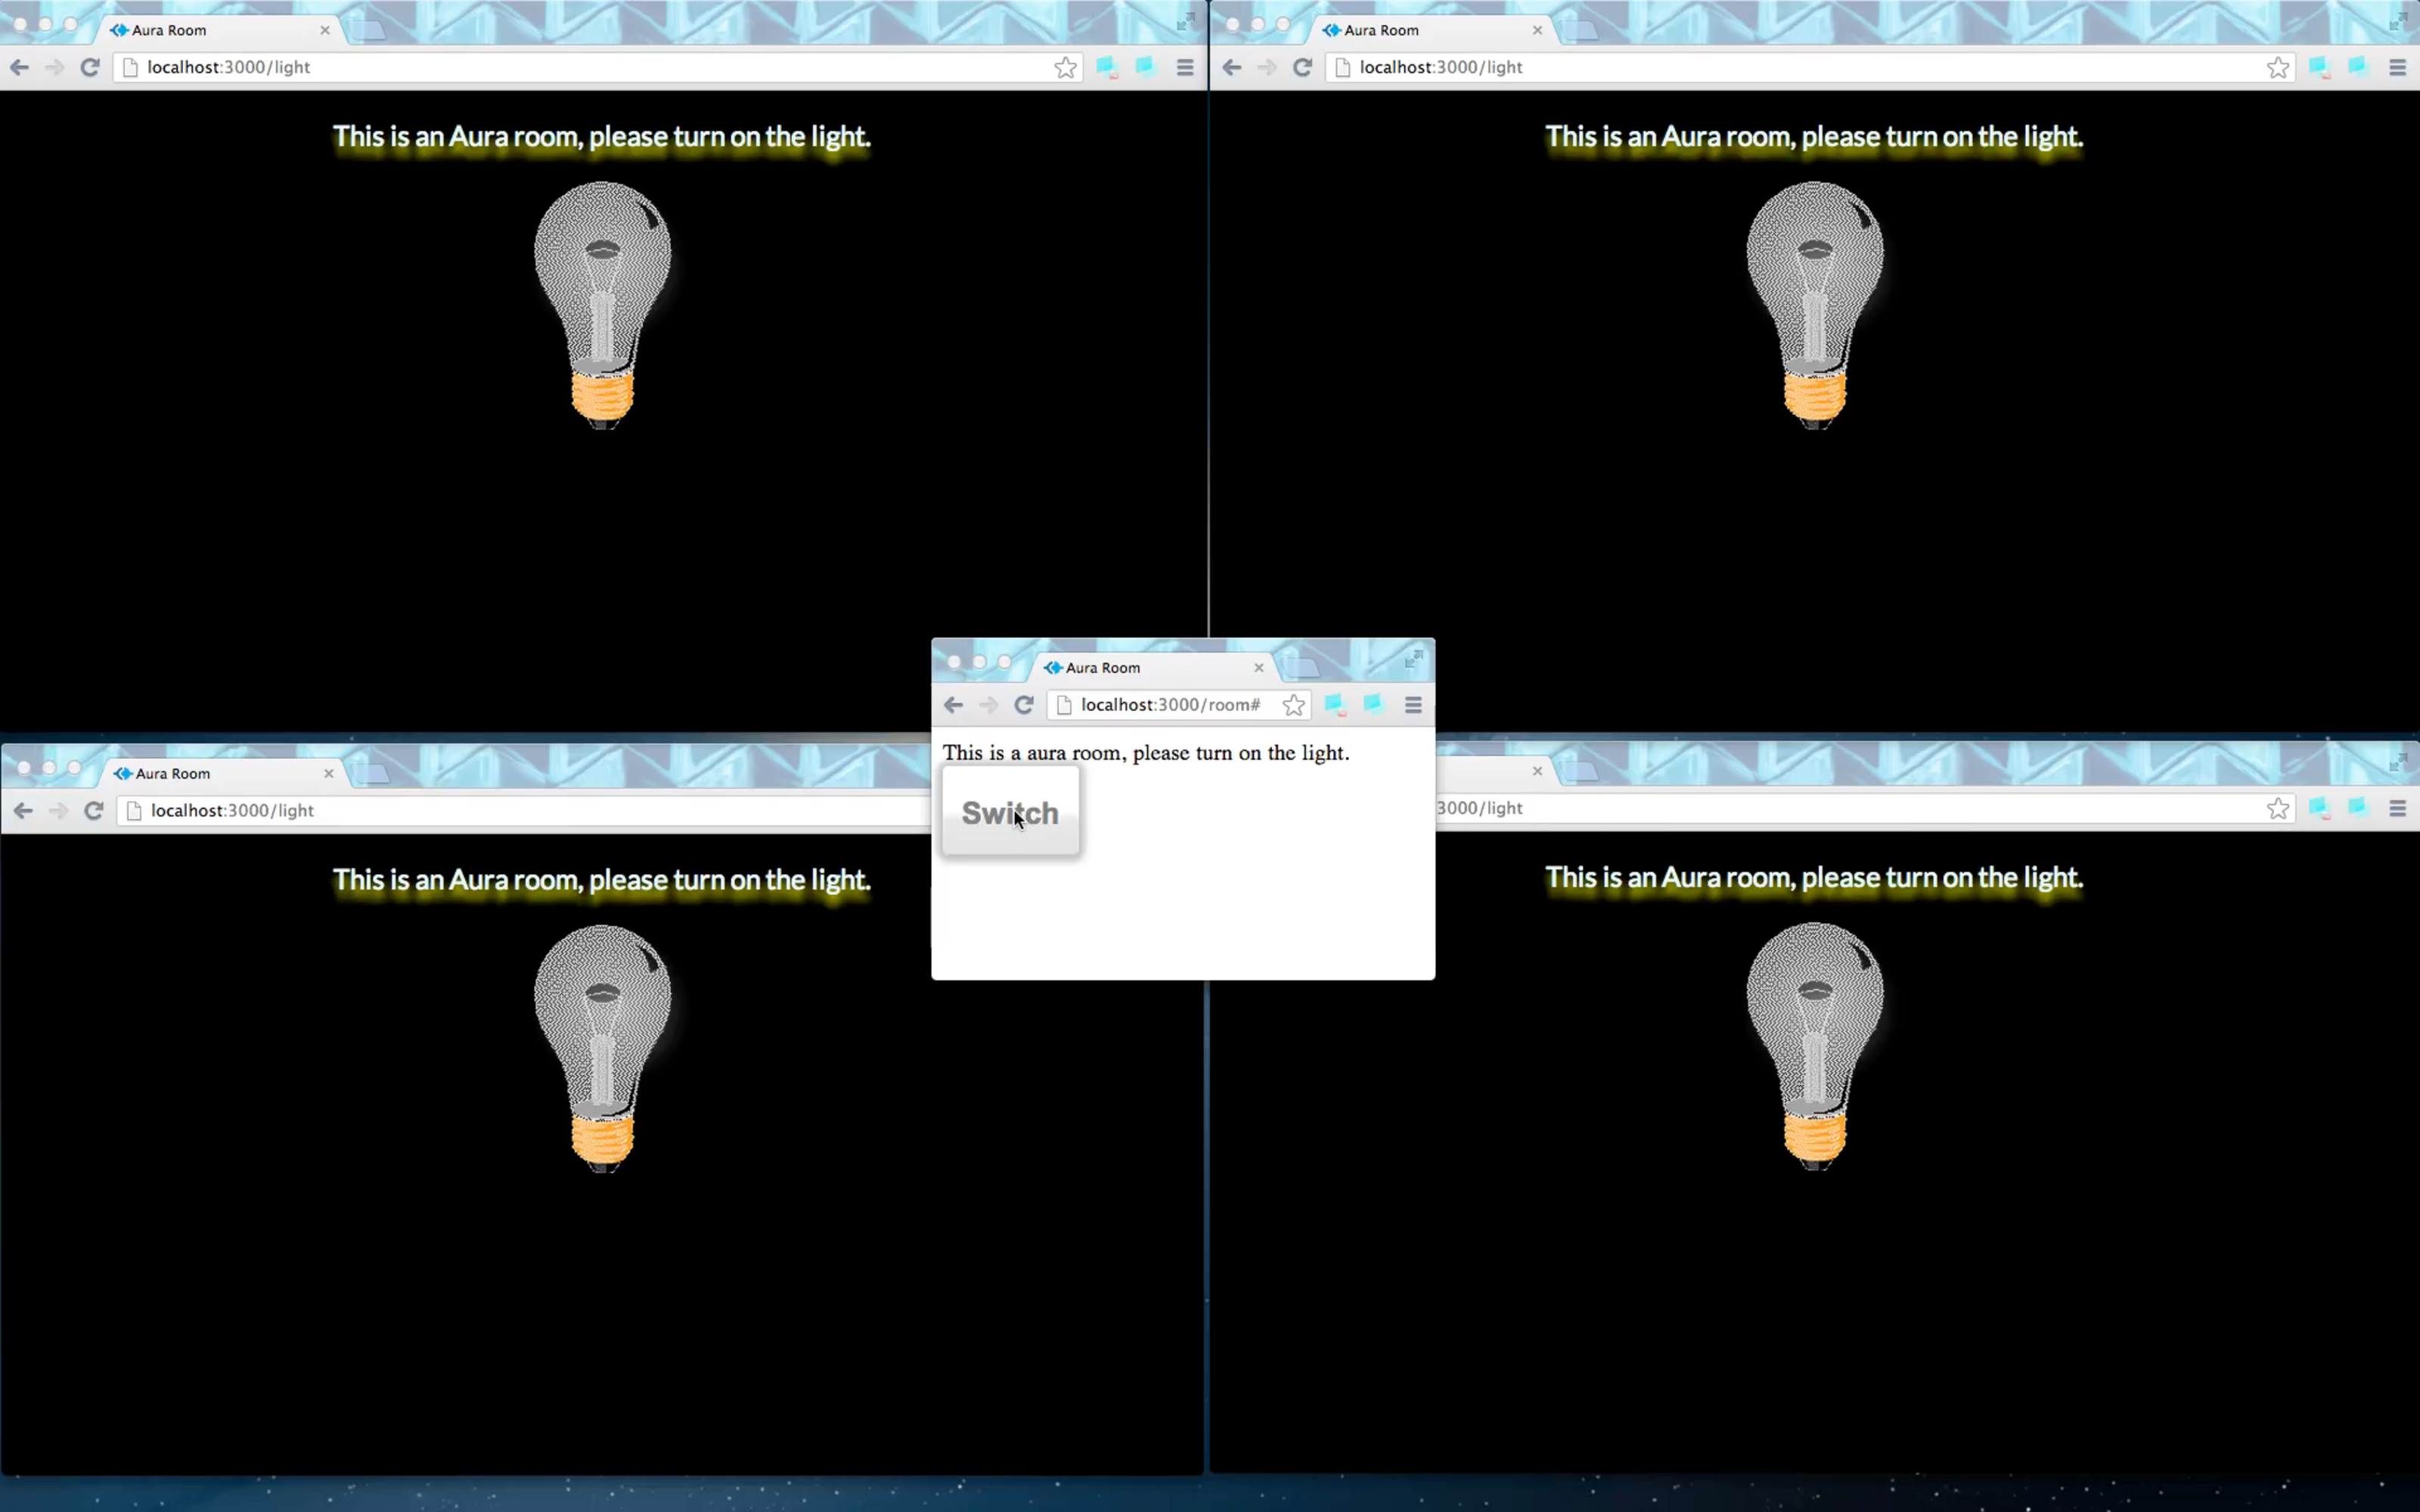
\includegraphics[width=1\textwidth]{images/screen-shot-home-auto-2.pdf}
    \caption{Visualisation of Remote Controlling Lights}
    \label{fig:screen-shot-home-auto-2}
  \end{center}
\end{figure}

\subsection{Social Sensing Application}

In this implementation, we built the customised web interface by using BackboneJS\footnote{http://backbonejs.org/}, which simplifies the process of handling data and connecting to the database. We also used D3\footnote{http://d3js.org/} library to visualise the data.

Figure \ref{fig:screen-shot-social-sensing-map} shows the social sensing application based on geo-location. The density of the nodes is visualised in heat map. This is, the colour scale is the reflection of the number of nodes at a place.

\begin{figure}[t]
  \begin{center}
    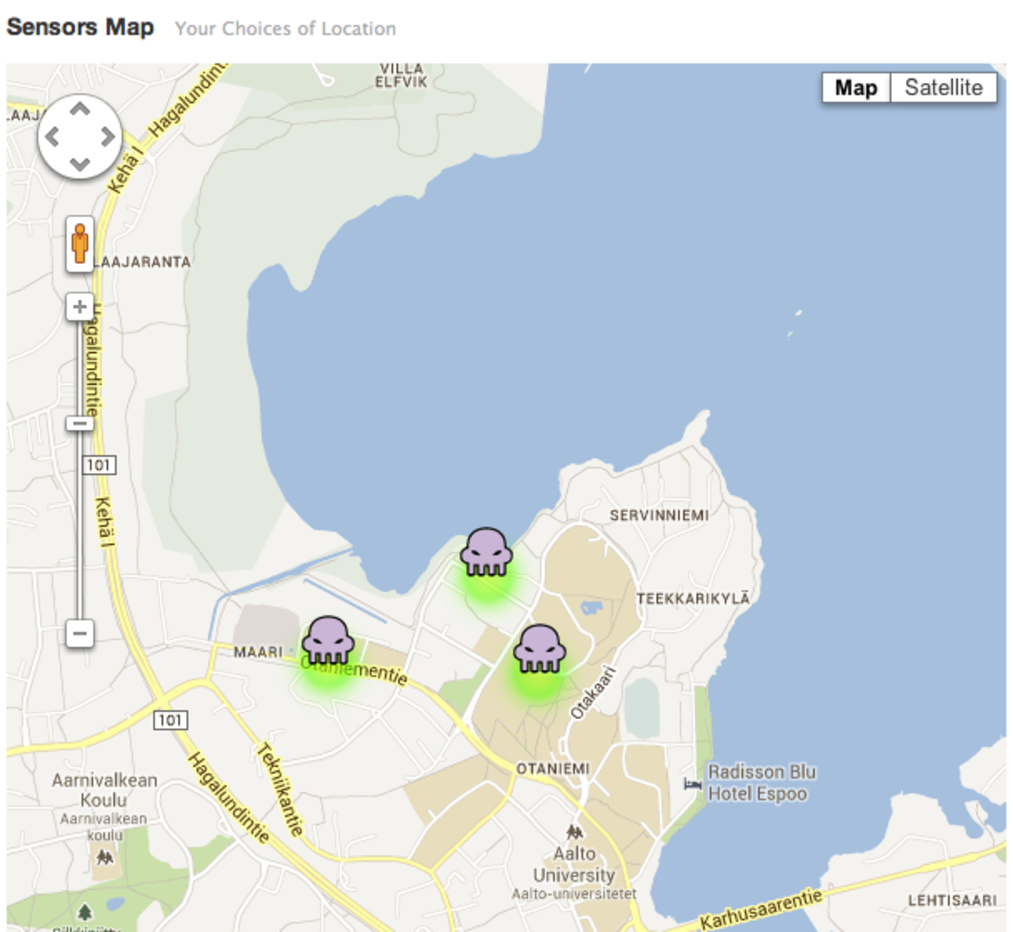
\includegraphics[width=1\textwidth]{images/screen-shot-social-sensing-map.pdf}
    \caption{Visualisation of Social Sensing based on Geo-location}
    \label{fig:screen-shot-social-sensing-map}
  \end{center}
\end{figure}

Figure \ref{fig:screen-shot-social-sensing-netowrk} shows the social sensing application based on nodes interconnection.

\begin{figure}[t]
  \begin{center}
    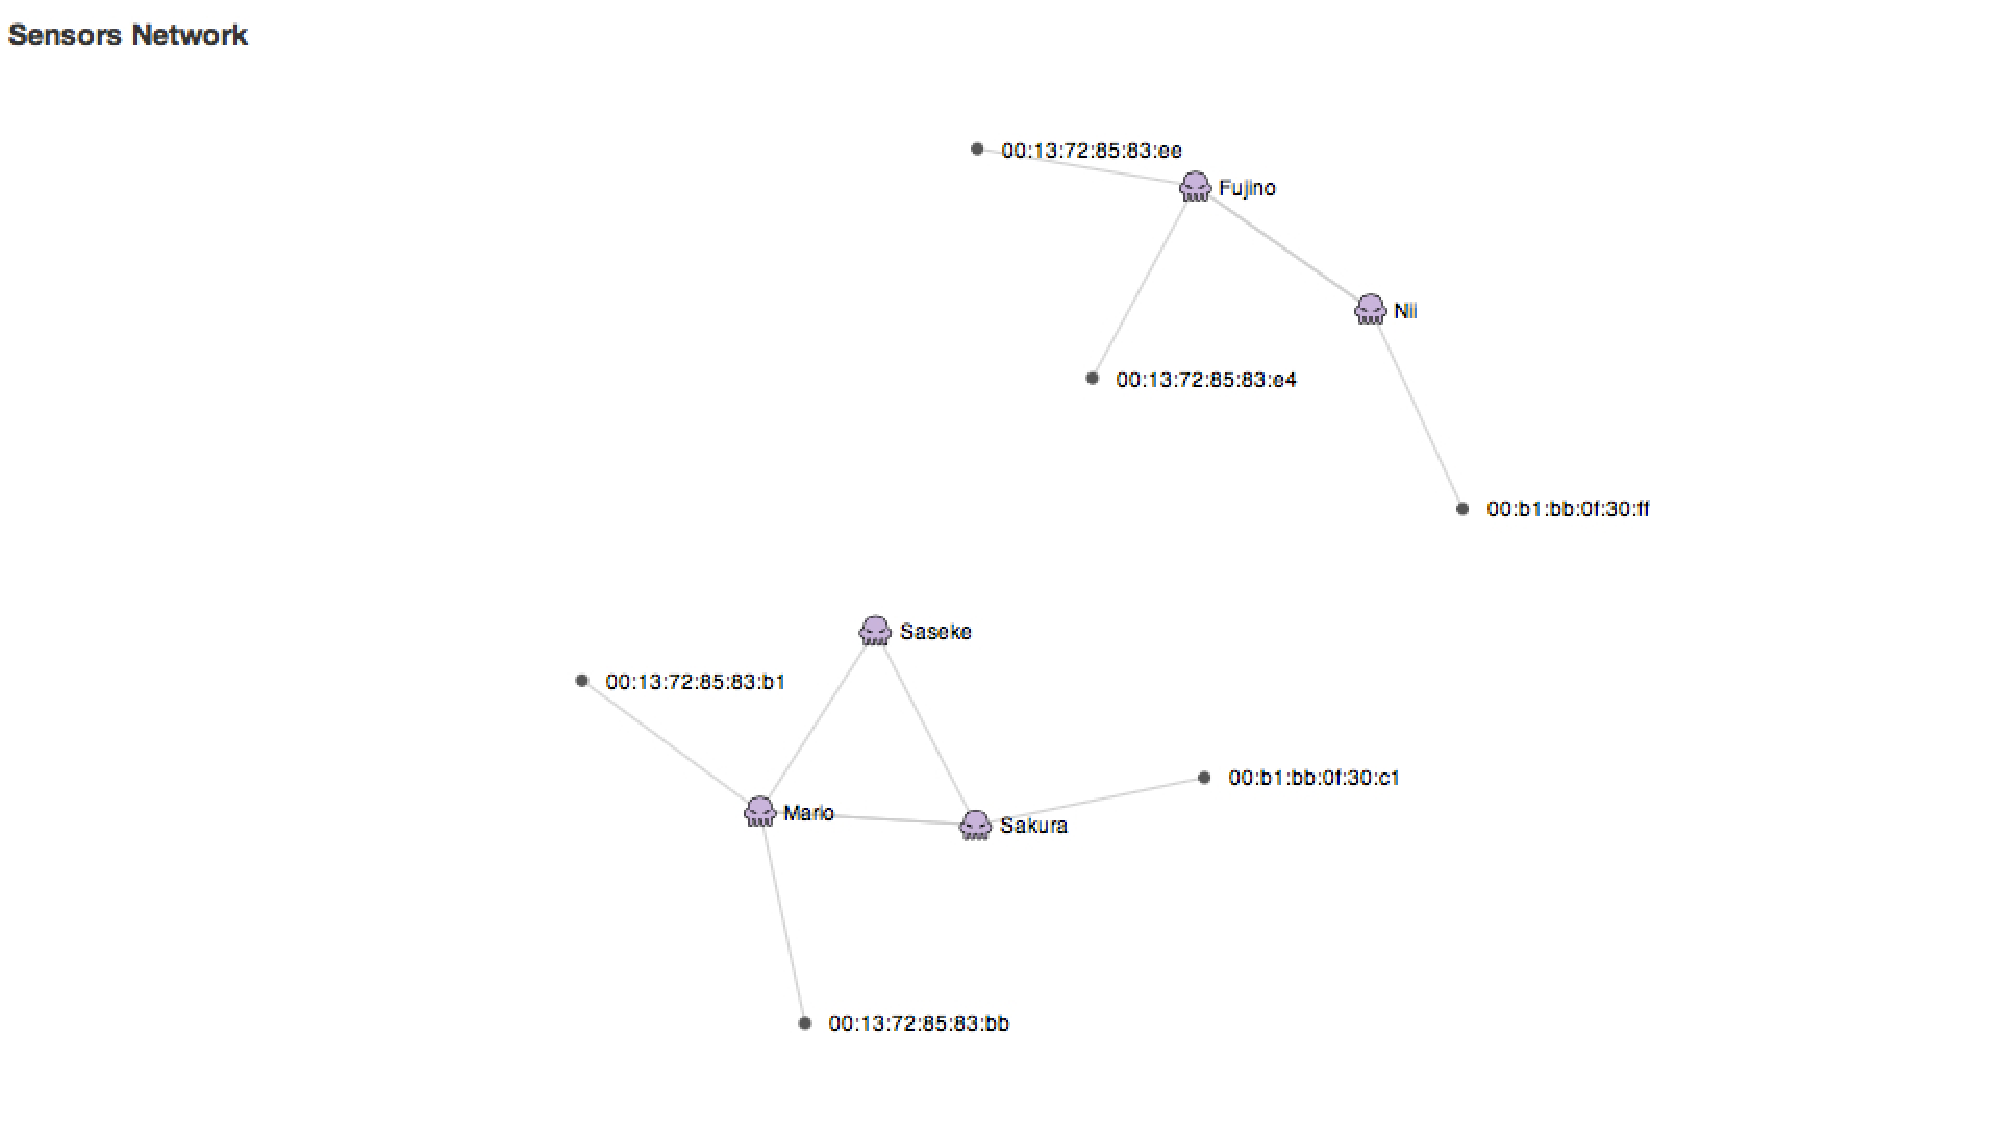
\includegraphics[width=1\textwidth]{images/screen-shot-social-sensing-netowrk.pdf}
    \caption{Visualisation of Social Sensing based on Nodes Interconnection}
    \label{fig:screen-shot-social-sensing-netowrk}
  \end{center}
\end{figure}
Figure \ref{fig:screen-shot-social-sensing-network-data} shows the visualisation of data in database-centric approach.

\begin{figure}[t]
  \begin{center}
    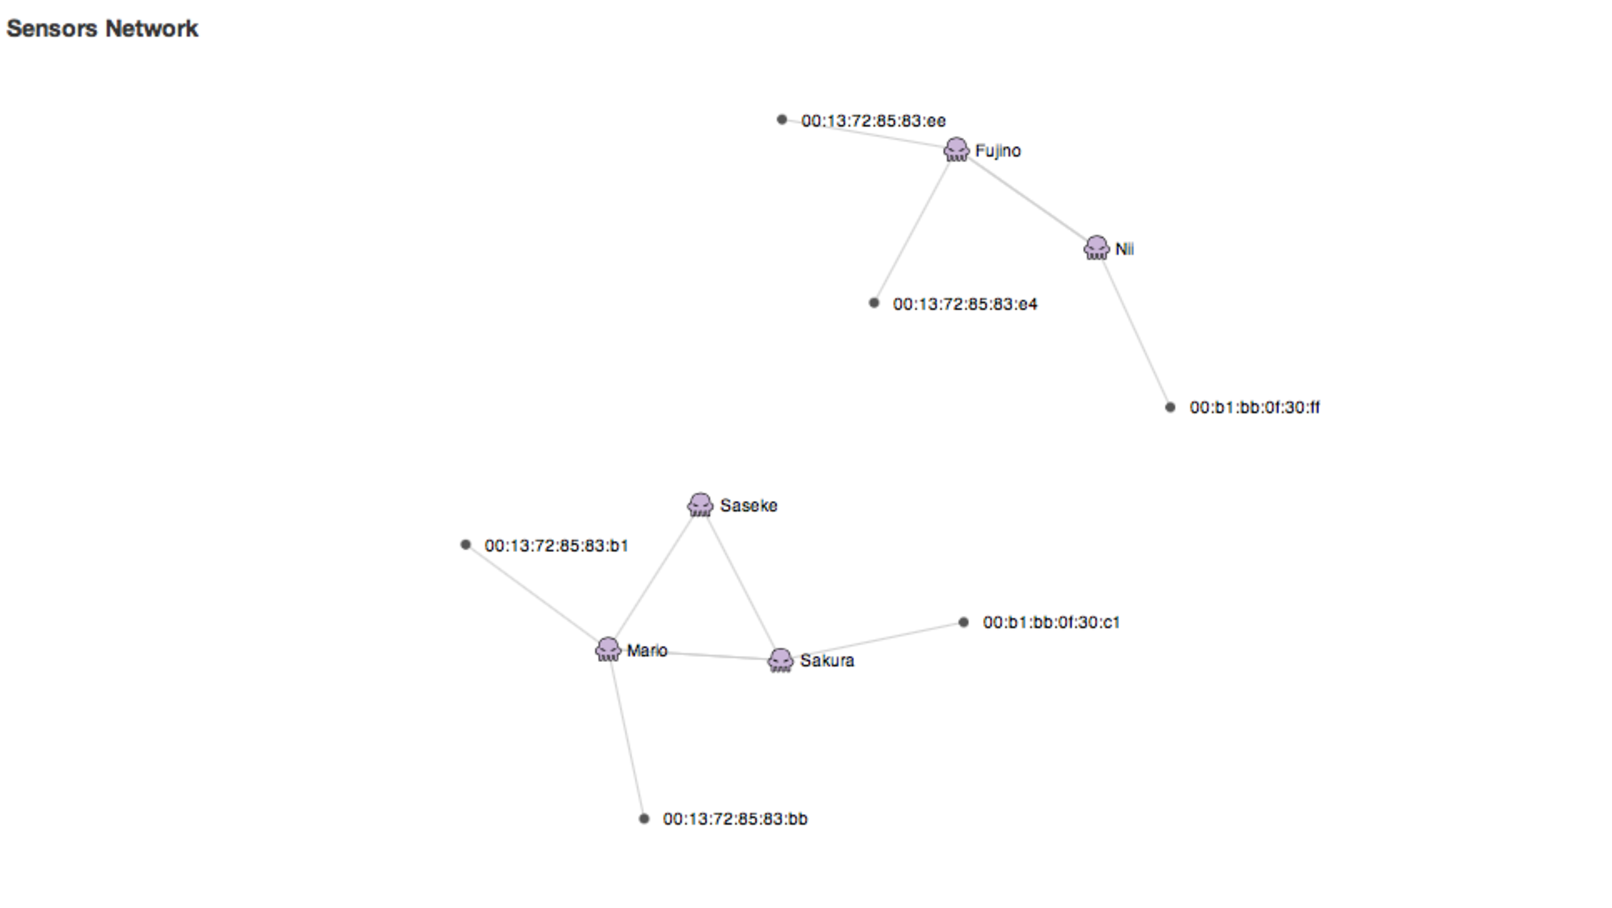
\includegraphics[width=1\textwidth]{images/screen-shot-social-sensing-network-data.pdf}
    \caption{Visualisation of Data in Database-centric Approach}
    \label{fig:screen-shot-social-sensing-network-data}
  \end{center}
\end{figure}

\end{appendices}



% End of document!
% ------------------------------------------------------------------
% The LastPage package automatically places a label on the last page.
% That works better than placing a label here manually, because the
% label might not go to the actual last page, if LaTeX needs to place
% floats (that is, figures, tables, and such) to the end of the 
% document.
\end{document}
